\documentclass{scrbook}
%\hypersetup{colorlinks}% uncomment this line if you prefer colored hyperlinks (e.g., for onscreen viewing)
%% Check out the stuff commented with three %'s

\usepackage[margin=1.2in]{geometry}
\usepackage[english]{babel}
\usepackage[utf8]{inputenc}
\usepackage[T1]{fontenc}
\usepackage{lmodern}
\usepackage{amsmath}
\usepackage{graphicx}
%\usepackage{indentfirst}
\usepackage{subcaption}
%\usepackage{fancyhdr}
\usepackage{textcomp}
\usepackage{comment}
\usepackage{mathtools}
\usepackage{amsfonts}
\usepackage{float}
\usepackage{amssymb}
\usepackage{cancel}
\usepackage[framemethod=tikz]{mdframed}
\usepackage{hyperref}
% \usepackage[pdftex,
%             pdfauthor={Prof. Vikram M. Gadre},
%             pdftitle={EE210X Book},
%             pdfsubject={Signals and Systems}]{hyperref}
% \pagestyle{fancy}
% \lhead{IITBombayX}
% \rhead{EE210.1X}
%\cfoot{\thepage}
%\renewcommand{\headrulewidth}{0.4pt}
%\renewcommand{\footrulewidth}{0.4pt}

% Book metadata
\title{\Huge Signals and Systems}
\author{\Large Dr. Vikram Gadre}
%\publisher{Publisher of This Book}
%%%\usepackage{booktabs}
\usepackage{graphicx}
%%%\setkeys{Gin}{width=\linewidth,totalh.eight=\textheight,keepaspectratio}
\graphicspath{{graphics/}}
%
\newcommand{\blankpage}{\newpage\hbox{}\thispagestyle{empty}\newpage}
% Generates the index
\usepackage{makeidx}
\makeindex
\begin{document}

% Front matter
\frontmatter

% r.1 blank page
%\blankpage
% r.3 full title page
\maketitle

\begin{comment}
% v.4 copyright page
\newpage
\begin{fullwidth}
~\vfill
\thispagestyle{empty}
\setlength{\parindent}{0pt}
\setlength{\parskip}{\baselineskip}
Copyright \copyright\ \the\year\ \thanklessauthor

\par\smallcaps{Published by \thanklesspublisher}

\par\smallcaps{tufte-latex.googlecode.com}

\par Licensed under the Apache License, Version 2.0 (the ``License''); you may not
use this file except in compliance with the License. You may obtain a copy
of the License at \url{http://www.apache.org/licenses/LICENSE-2.0}. Unless
required by applicable law or agreed to in writing, software distributed
under the License is distributed on an \smallcaps{``AS IS'' BASIS, WITHOUT
WARRANTIES OR CONDITIONS OF ANY KIND}, either express or implied. See the
License for the specific language governing permissions and limitations
under the License.\index{license}

%\par\textit{First printing, \monthyear}
\end{fullwidth}
\end{comment}
% r.5 contents
\tableofcontents

\listoffigures

\listoftables

\begin{comment}
% r.7 dedication
\cleardoublepage
~\vfill
\begin{doublespace}
\noindent\fontsize{18}{22}\selectfont\itshape
\nohyphenation
Dedicated to those who appreciate \LaTeX{} 
and the work of \mbox{Edward R.~Tufte} 
and \mbox{Donald E.~Knuth}.
\end{doublespace}
\vfill
\vfill
\end{comment}

% r.9 introduction
\cleardoublepage
\mainmatter
\part{Frequency Domain}
\chapter{Sinusoids and LSI Systems}
\section{Module 2: Lecture 1\\Sinusoidal Signals and their Properties}

\subsection*{Introduction}
In the first module, we have been looking at signals and systems in what is
called their natural domain. By natural domain, we mean that the independent
variable of the signal is the same as it was when the signal was
recorded or observed or instituted. An example of a signal in its natural
domain is a speech signal expressed as a function of time, as time is the
naturally associated independent variable with the speech signal. \\
For processing signals, we need appropriate systems. Now, what processing needs to be done by the system can be a tricky thing to specify in the
natural domain. \\
For example, say we want to separate the voices of male and female
singers from an audio recording of a chorus. Although it is qualitatively easier to understand, one can't give the description of such a system in the
time domain. We need to
have a broader view of systems, and more importantly, of signals, to be able
to tackle this problem. \\
So in this module we are going to take the first step towards a change of
paradigm, a change of world-view in describing signals and systems.
%% Adding the Introduction from M2L02 here as of now.
In this lecture we will learn how to deal with phase changes in sinusoidal signals and pass sinusoidal signals into stable LSI systems in an intelligent and insightful manner. We will look into why we introduced complex signals in our previous analysis and how these tools make the mathematical modelling simple. We then go on to understanding how to deal with signals beyond the domain of sinusoids.
%% Intro of M2L02 ends here
We begin by understanding which signals are special from the point of view of
the signals and systems. Let's visit the ideal voltage generator for that
purpose.
\subsection{The Ideal Voltage generator}
The ideal voltage generator consists of a circular conducting coil rotating in
a constant magnetic field.
\begin{figure}[ht]
\centering
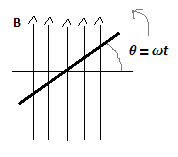
\includegraphics{flux.png}
\caption{\label VVoltage generator (side view)}
\end{figure}
\\
Let the area enclosed by the coil be $A$, the angular frequency of
rotation be $\omega$ such that $\theta = \omega t$, and the value of the
constant magnetic field be $B$. Now, by Faraday's law, the electric field $\mathcal{E}$ is defined as
\[ \mathcal{E}= - \frac{\partial \Phi_B}{\partial t} \]
where the flux $\Phi_B$ in this case is given by
\[ \Phi_B = BA \cos \theta = BA \cos \omega t \]
Hence the electric field will be
\[ \mathcal{E}= - BA \ \omega \sin \omega t \]
This is the principle of generation of the voltage supply that we receive at
our residences. This is one important reason why the sinusoidal voltage is
highly favoured and deeply studied. And of course there are many other reasons
why. Let us have a look at some interesting properties of sinusoids.
%%%
%%%
\subsection{Properties of sinusoids}
The first interesting thing about sine waves is that when you add two sinusoids
of the same frequency, it gives you back another sinusoid of the \emph{same}
frequency. Let's prove this formally.
Say we have two sinusoids, $x_1 (t)$ and $x_2 (t)$, of the same angular frequency
$\Omega,$ given by
\begin{equation*}
x_1 (t) = A_1 \cos (\Omega t + \phi_1)
\end{equation*}
\begin{equation*}
x_2 (t) = A_2 \cos (\Omega t + \phi_2)
\end{equation*}
Now consider a linear combination of the two sinusoids,
\begin{equation*}
x (t) = \alpha_1 x_1 (t) + \alpha_2 x_2 (t)
\end{equation*}
Note that we can write $x_1$ and $x_2$ as
\begin{equation*}
x_1 (t) = A_1  \{ \cos \Omega t \cos \phi_1 - \sin \Omega t \sin \phi_1 \}
\end{equation*}
\begin{equation*}
x_2 (t) = A_2  \{ \cos \Omega t \cos \phi_2 - \sin \Omega t \sin \phi_2 \}
\end{equation*}
Hence we can write $x (t)$ as
\begin{equation*}
x (t) = [ \alpha_1 A_1 \cos \phi_1 + \alpha_2 A_2 \cos \phi_2 ] \cos
   \Omega t + [ - \alpha_1 A_1 \sin \phi_1 - \alpha_2 A_2 \sin
   \phi_2 ] \sin \Omega t
\end{equation*}
Writing the two time-independent coefficients as $P$ and $Q$, we get
\begin{equation*}
 x (t) = P \cos \Omega t + Q \sin \Omega t = \sqrt{P^2 + Q^2}  \left\{
   \frac{P}{\sqrt{P^2 + Q^2}} \cos \Omega t + \frac{Q}{\sqrt{P^2 + Q^2}}
   \sin \Omega t \right\}
\end{equation*}
This can be easily seen to be
\begin{equation*}
 x (t) = \sqrt{P^2 + Q^2} \cos (\Omega t + \Phi)
\end{equation*}
with
\begin{equation*}
\Phi = - \tan^{- 1} \left( \frac{Q}{P} \right)
\end{equation*}
Hence, linearly combining two sinusoids of the same frequency gives back a
sinusoid with the same frequency.\\
Another interesting property is that when we differentiate a
sine wave, we get back a sinusoid of the same frequency.
\begin{equation*}
\frac{d}{d t}  \{ A \cos (\Omega t + \phi) \} = - A \Omega \sin
   (\Omega t + \phi)
\end{equation*}
It doesn't matter whether it is cosine or sine since they differ only by a
phase of $\pi / 2$.
\[ \cos (\Omega t + \phi) = \sin (\Omega t + \phi + \pi / 2) \]
Now let's see how we can describe a change in amplitude of a sinusoid.
Suppose the original sinusoid is given by
\[ x_1 (t) = A \cos (\Omega t + \phi) \]
and let the changed sinusoid is given by
\[ x_2 (t) = B \cos (\Omega t + \phi) \]
where $A$ and $B$ are positive constants. Then,
\[ x_2 (t) = \frac{B}{A} x_1 (t) \]
So the change of amplitude in a sinusoid is simply described by a multiplying
constant.\\
But this is not true for a phase change. Suppose the original sinusoid is
given by
\[ x_1 (t) = A \cos (\Omega t + \phi_1) \]
and the changed sinusoid is given by
\[ x_2 (t) = A \cos (\Omega t + \phi_2) \]
Unlike the amplitude case, $x_2 (t) / x_1 (t)$ doesn't turn out to be a
constant independent of time. This will cause a problem while dealing with
inductors or capacitors. In inductors, for example, the voltage drop is
proportional to the derivative of the current passing through it. Hence, if a
sinusoidal current is passing through it, the voltage drop across it will also
be a sinusoid, but will have a phase difference of $90^0$ with the current.
Hence, we cannot establish a relationship like the resistor $(V = RI)$ in case
of the inductor since $V / I$ won't be a constant independent of time.\\
To deal with this problem, we will have to use the rotating complex number
representation of the sinusoid.

\subsection{Sinusoids as Rotating Complex Numbers}

We can think of a sinusoid $I_0 \cos (\Omega t + \phi_0)$ as a combination of
two rotating complex numbers. Let the first begin at time $t = 0$ with an
angle of $\phi_0$. Let it have a magnitude of $I_0 / 2$ and let the other
begin with the same magnitude $I_0 / 2$ but the opposite starting angle ($-
\phi_0$). Let them both rotate with an angular velocity of $\Omega$, but the
first one in counter clockwise and the second one in clockwise direction.
\begin{figure}[ht]
\centering
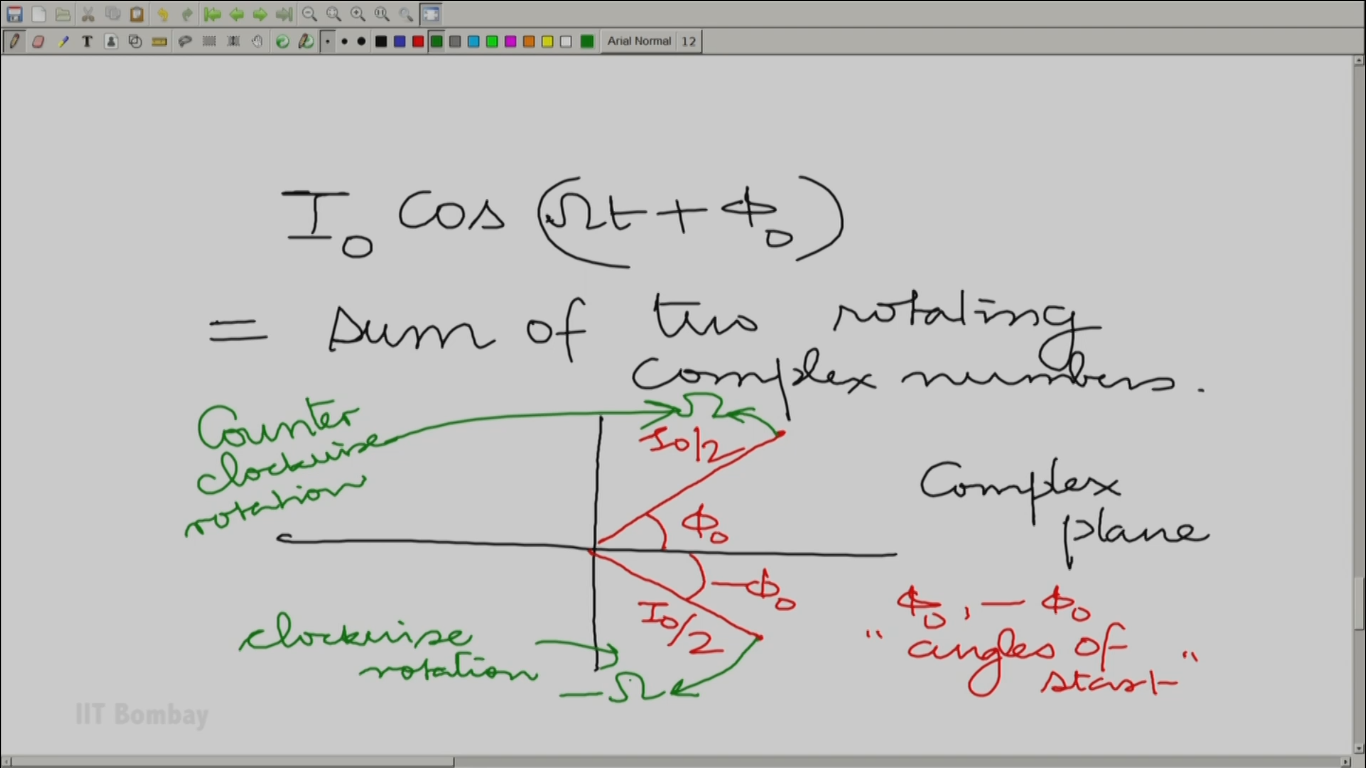
\includegraphics[scale=0.28]{rotating_complex.png}
\end{figure}
\\
We can express these two complex numbers in the polar form as
\[ c_1 = \frac{I_0}{2} e^{j \{ \Omega t + \phi_0 \}} \]
\[ c_2 = \frac{I_0}{2} e^{- j \{ \Omega t + \phi_0 \}} \]
where $j = \sqrt{- 1}$. One can see that $c_1 + c_2$ gives back the original
sinusoid.\\
It seems like a silly thing to do to describe a sinusoid as a combination of
two rotating complex numbers. But the reason for doing this is clear when we
look at the inductor once again.\\
Let's assume for now that we provide to the inductor, an input which is just
one of those rotating complex numbers. So
\[ I = \frac{I_0}{2} e^{j \{ \Omega t + \phi_0 \}} \]
Now, the voltage across an inductor is given by
\[ V = L \frac{d I}{d t} = L\frac{I_0}{2} (j \Omega) e^{j \{ \Omega t +
   \phi_0 \}} \]
Hence we can see that
\[ V / I = j \Omega L \]
Now the ratio of the voltage and current for an inductor is a complex
\textit{constant independent of time}!\\
Similarly, for the other rotating complex number, we will get $V / I$ again to
be a constant, but with a minus sign $(- j \Omega L)$. So in some sense the
actual angular frequency, whether positive or negative, is reflected. It is left as an exercise to do a similar analysis for capacitances and verify that
for capacitors,
\[ V / I = \frac{1}{j \Omega C} \]
This makes the analysis of RLC circuits (circuits consisting of Resistor(s),
Inductor(s) and Capacitors(s)) much easier as we can interpret these constants
as generalised resistances, or \textit{impedances.} In that sense, the
resistor has an impedance of $R$, an inductor has an inductance of $j \Omega
L$ and a capacitor has an impedance of $1 / j \Omega C$.\\
Notice that $c_1$ and $c_2$ defined above are complex conjugates of each
other. So whatever happens to $c_1$ is mirrored in $c_2$. For example, the $V
/ I$ for $c_2$ ($- j \Omega L$) is the complex conjugate of the $V / I$ for
$c_1$ ($j \Omega L$).\\
The analysis of sinusoids using rotating complex numbers is known as `phasor'
analysis. As the rotating complex numbers are constant in magnitude, but
change their phase, they are called `phasors'.\\
This is the reason why we earlier demanded that our systems should accept a
complex signal in general.\\
In a nutshell, dealing with amplitudes is easy but the dealing with phases is
a problem in sinusoids and that problem is overcame when you go to the phasor
instead of the corresponding sinusoid. Let us see how a general LSI system responds to
a phasor or sinusoid as an input.
\section{Module 2: Lecture 2\\Sinusoidal Input to LSI Systems}


%\subsection{Introduction}

\subsection{Understanding Phase Change In Sinusoids and Phasors}
We write a sinusoid as a combination of two rotating complex numbers, which we will henceforth call phasors, moving in opposite directions. 
\[
	2Acos(\Omega t + \phi) = Ae^{j(\Omega t + \phi)} + Ae^{-j(\Omega t + \phi)}
\]
Let us focus our attention on one of the phasors for now. Let us look at what happens when we introduce a phase change.\\
\[
Ae^{j(\Omega t + \phi)} \xrightarrow{Phase \ Change} Ae^{j(\Omega t + \phi + \Delta\phi)}
\]
\[
Ae^{j(\Omega t + \phi + \Delta\phi)} =
Ae^{j(\Omega t + \phi)}e^{j\Delta\phi}
\]
We hence find that a change of phase results just in a multiplying factor which is a constant independent of time.\\
Now we try to do a similar calculation for the complex conjugate (the phasor moving in the opposite direction).
\[
Ae^{-j(\Omega t + \phi)} \xrightarrow{Phase \ Change} Ae^{-j(\Omega t + \phi)}e^{-j\Delta\phi}
\]
Notice that the multiplying constant in this case is the complex conjugate of the previous multiplying factor we found.\\
\[
	2Acos(\Omega t + \phi) \xrightarrow{Phase \ Change} Ae^{j(\Omega t + \phi)}e^{j\Delta\phi} + Ae^{-j(\Omega t + \phi)}e^{-j\Delta\phi}
\]
We hence understand that using only one phasor is enough to fully determine the behaviour of the sinusoid. This explains why we used complex signals in our previous analysis, due to their ease in mathematical manipulation.\\
We will now see the result of inputting a sinusoidal signal to a stable linear shift invariant system, with impulse response $h(t)$ (Assume that the impulse response is real). We deal with stable LSI systems because the output will be bounded.\\
\begin{figure}[ht]
\begin{center}
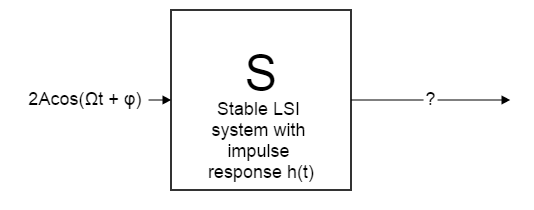
\includegraphics[width=10cm]{LSIcos.png}
\caption{Sinusoidal Input To Stable LSI System}
\end{center}
\end{figure}
The output for an LSI system is given by the convolution of the input and the impulse response.
The direct solution via convolution seems very difficult. In fact if we try to calculate the convolution integral, we get the following expression:
\[
y(t) = \int_{-\infty}^{+\infty} \! {h(\lambda)2Acos(\Omega(t-\lambda) + \phi) \ \dm \lambda}\]
We will now see how to solve it using phasors, making the analysis mathematically convenient.
%%%
%%%
\subsection{Phasor Input to LSI System}
Consider the output when a phasor is input to a stable LSI system.
\[
Ae^{j(\Omega t + \phi)} \xrightarrow{LSI} 
 \int_{\infty}^{\infty} \! Ae^{j(\Omega (t - \lambda) + \phi)}h(\lambda) \ \dm \lambda
\]
 
\[ =
Ae^{j(\Omega t + \phi)} \int_{\infty}^{\infty} \! {e^{-j\Omega\lambda}h(\lambda) \ \dm \lambda}
\]
Here, we see that we get the output to be the input phasor with a multiplying factor $\int_{-\infty}^{\infty} \! {e^{-j\Omega\lambda}h(\lambda) \ \dm \lambda}$, which is dependent only on $\Omega$ and $h$ (it is constant with respect to time).\\
We will now come back to the importance of why we chose our system to be stable. We will do this by trying to find a bound to the absolute value of the multiplying factor we just found.
\[
| \int_{-\infty}^{\infty} \! {e^{-j\Omega\lambda}h(\lambda) \ \dm \lambda} | \leq 
\int_{-\infty}^{\infty} \! { |e^{-j\Omega\lambda}||h(\lambda)| \ \dm \lambda }
\]
\[
\int_{-\infty}^{\infty} \! { |e^{-j\Omega\lambda}||h(\lambda)| \ \dm \lambda } =
\int_{-\infty}^{\infty} \! {|h(\lambda)| \ \dm \lambda }
\]
And as per the condition of stability the integral of the absolute value of the impulse response is bounded. Hence the absolute value of the multiplying factor is also bounded. In fact we have obtained a concrete bound to this integral, namely the absolute integral of the impulse response. We can do similar mathematical analysis for the conjugate as well.\\
This multiplying factor is called the \textit{Frequency Response} of the LSI system at angular frequency $\Omega$.
\[
	Frequency\ Response\ H(\Omega) = \int_{-\infty}^{\infty} \! {e^{-j\Omega\lambda}h(\lambda) \ \dm \lambda}
\] 
%%%
%%%
\subsection{Sinusoid Input to LSI System}
We will now come back to our original problem of inputting a sinusoidal signal into a stable linear shift invariant system. We will begin by simplifying the outputs of the two phasors.
\[
	H(\Omega)Ae^{j(\Omega t + \phi)} = |H(\Omega)|Ae^{j(\Omega t + \phi +  \angle  H(\Omega))}
\]
The complex conjugate of the frequency response is given by
\[
\bar{H}(\Omega) = \int_{-\infty}^{\infty} \! {e^{j\Omega\lambda}h(\lambda) \ \dm \lambda} = H(-\Omega)
\]
Note that the first equality holds only if $h(\lambda)$ is real.
Hence,
\[
H(-\Omega)Ae^{-j(\Omega t + \phi)} = |H(\Omega)|Ae^{-j(\Omega t + \phi +  \angle  H(\Omega))}
\]
So we can check by adding the two outputs that the output for inputting a sinusoid $2Acos(\Omega t + \phi)$ is given by:

\[
2Acos(\Omega t + \phi) \xrightarrow{Stable\ LSI} 2A|H(\Omega)|cos(\Omega t + \phi + \angle H(\Omega))
\]
This indicates that on passing through a stable LSI system, a sinusoid goes through an amplitude and phase shift which is independent of time and only dependent on the impulse response and angular frequency of the sinusoid. Note again that the impulse response has to be real for this to hold true.\\
Also, if we view an input to a stable LSI system as the sum of multiple sinusoids, the output can be visualized as the sum of the corresponding outputs of the sinusoids through the stable LSI system. The stability of the LSI systems guarantees the existence of the frequency response of the system. But if it is unstable it may or may not have a frequency response.
%%%
%%%
\subsection{Periodic Input to Shift Invariant Systems}
How does an LSI system respond to a general periodic signal? Consider the following lemma.\\
\textbf{Lemma:} A periodic input to a shift invariant system produces a periodic output.\\
\textbf{Proof:}\\
%%%
Let the input be $x(t)$ with a period $T$
\[x(t+T) = x(t)\ \ \forall t\]
\[x(t) \xrightarrow{SI\ system} y(t) \]
%%%
Now, by shift invariance,
\[x(t+T) \xrightarrow{SI\ system} y(t+T) \]
Hence,
\begin{equation}\label{eqn:PeriodicOutput}
y(t) = y(t+T)\ \ \forall \ t
\end{equation}
Hence the output is also periodic, infact with the same period $T$.\\
An important property of a periodic input or a periodic function is that it can be represented by a linear combination (which can be countably infinite) of sinusoids having frequencies which are multiples of the frequency of the input. This property is referred to as the existence of a Fourier Series expansion of the input. \\
The Fourier Series expansion and our understanding from the previous section gives us a simple method to compute the output of a periodic input in an LSI system as the linear combination of the output of these sinusoids.\\
%% Added paragraph for better flow. Needs verification:
This result, combined with \ref{eqn:PeriodicOutput} can be used to calculate the output for a general periodic input, but for that, we need still more information. How do we know whether a certain periodic signal can be expressed as a linear combination of sinusoids \emph{uniquely}? To answer this question, we need to invoke some concepts from linear algebra by considering signals as vectors.

%\subsection{Conclusion}
%In this lecture we understood the analysis of inputting sinusoidal input to a stable LSI system. We saw how we could simplify our analysis by the use of phasors. In the upcoming lecture we will learn about the use of inner product and vector analysis in understanding signals.


\section{Module 2: Lecture 3\\Signals and Vectors}

\subsection{Introduction}
In the previous lecture, we have learnt how a periodic input given to a Linear Shift Invariant system results in a periodic output with the same period. Now in this lecture we will see some new concepts by which every input can be expressed as sinusoidal inputs. Henceforth, it will be simpler to analyse their outputs.

\subsection{Relations between Signals and Vectors}
\label{sec:examples}
Consider a 2-dimensional vector, we can decompose this vector into two perpendicular components with $e_1$ and $e_2$ as the unit vectors along those directions. To find these components, we need to use Dot Product.
\subsubsection{Dot Product}
	Dot Product of two vectors u and v is defined as the magnitude of vector u multiplied by the magnitude of v multiplied by cosine of the angle between these two vectors.
    
	    					\begin{equation*}u.v = |u||v|cos\theta\end{equation*}
                            
where $\theta$ is the angle between vectors u and v. If u is a unit vector, then the dot product of vectors v and u gives the component of vector v in the direction of u, with the value |v|cos$\theta$.
	\begin{figure}[ht]
\centering
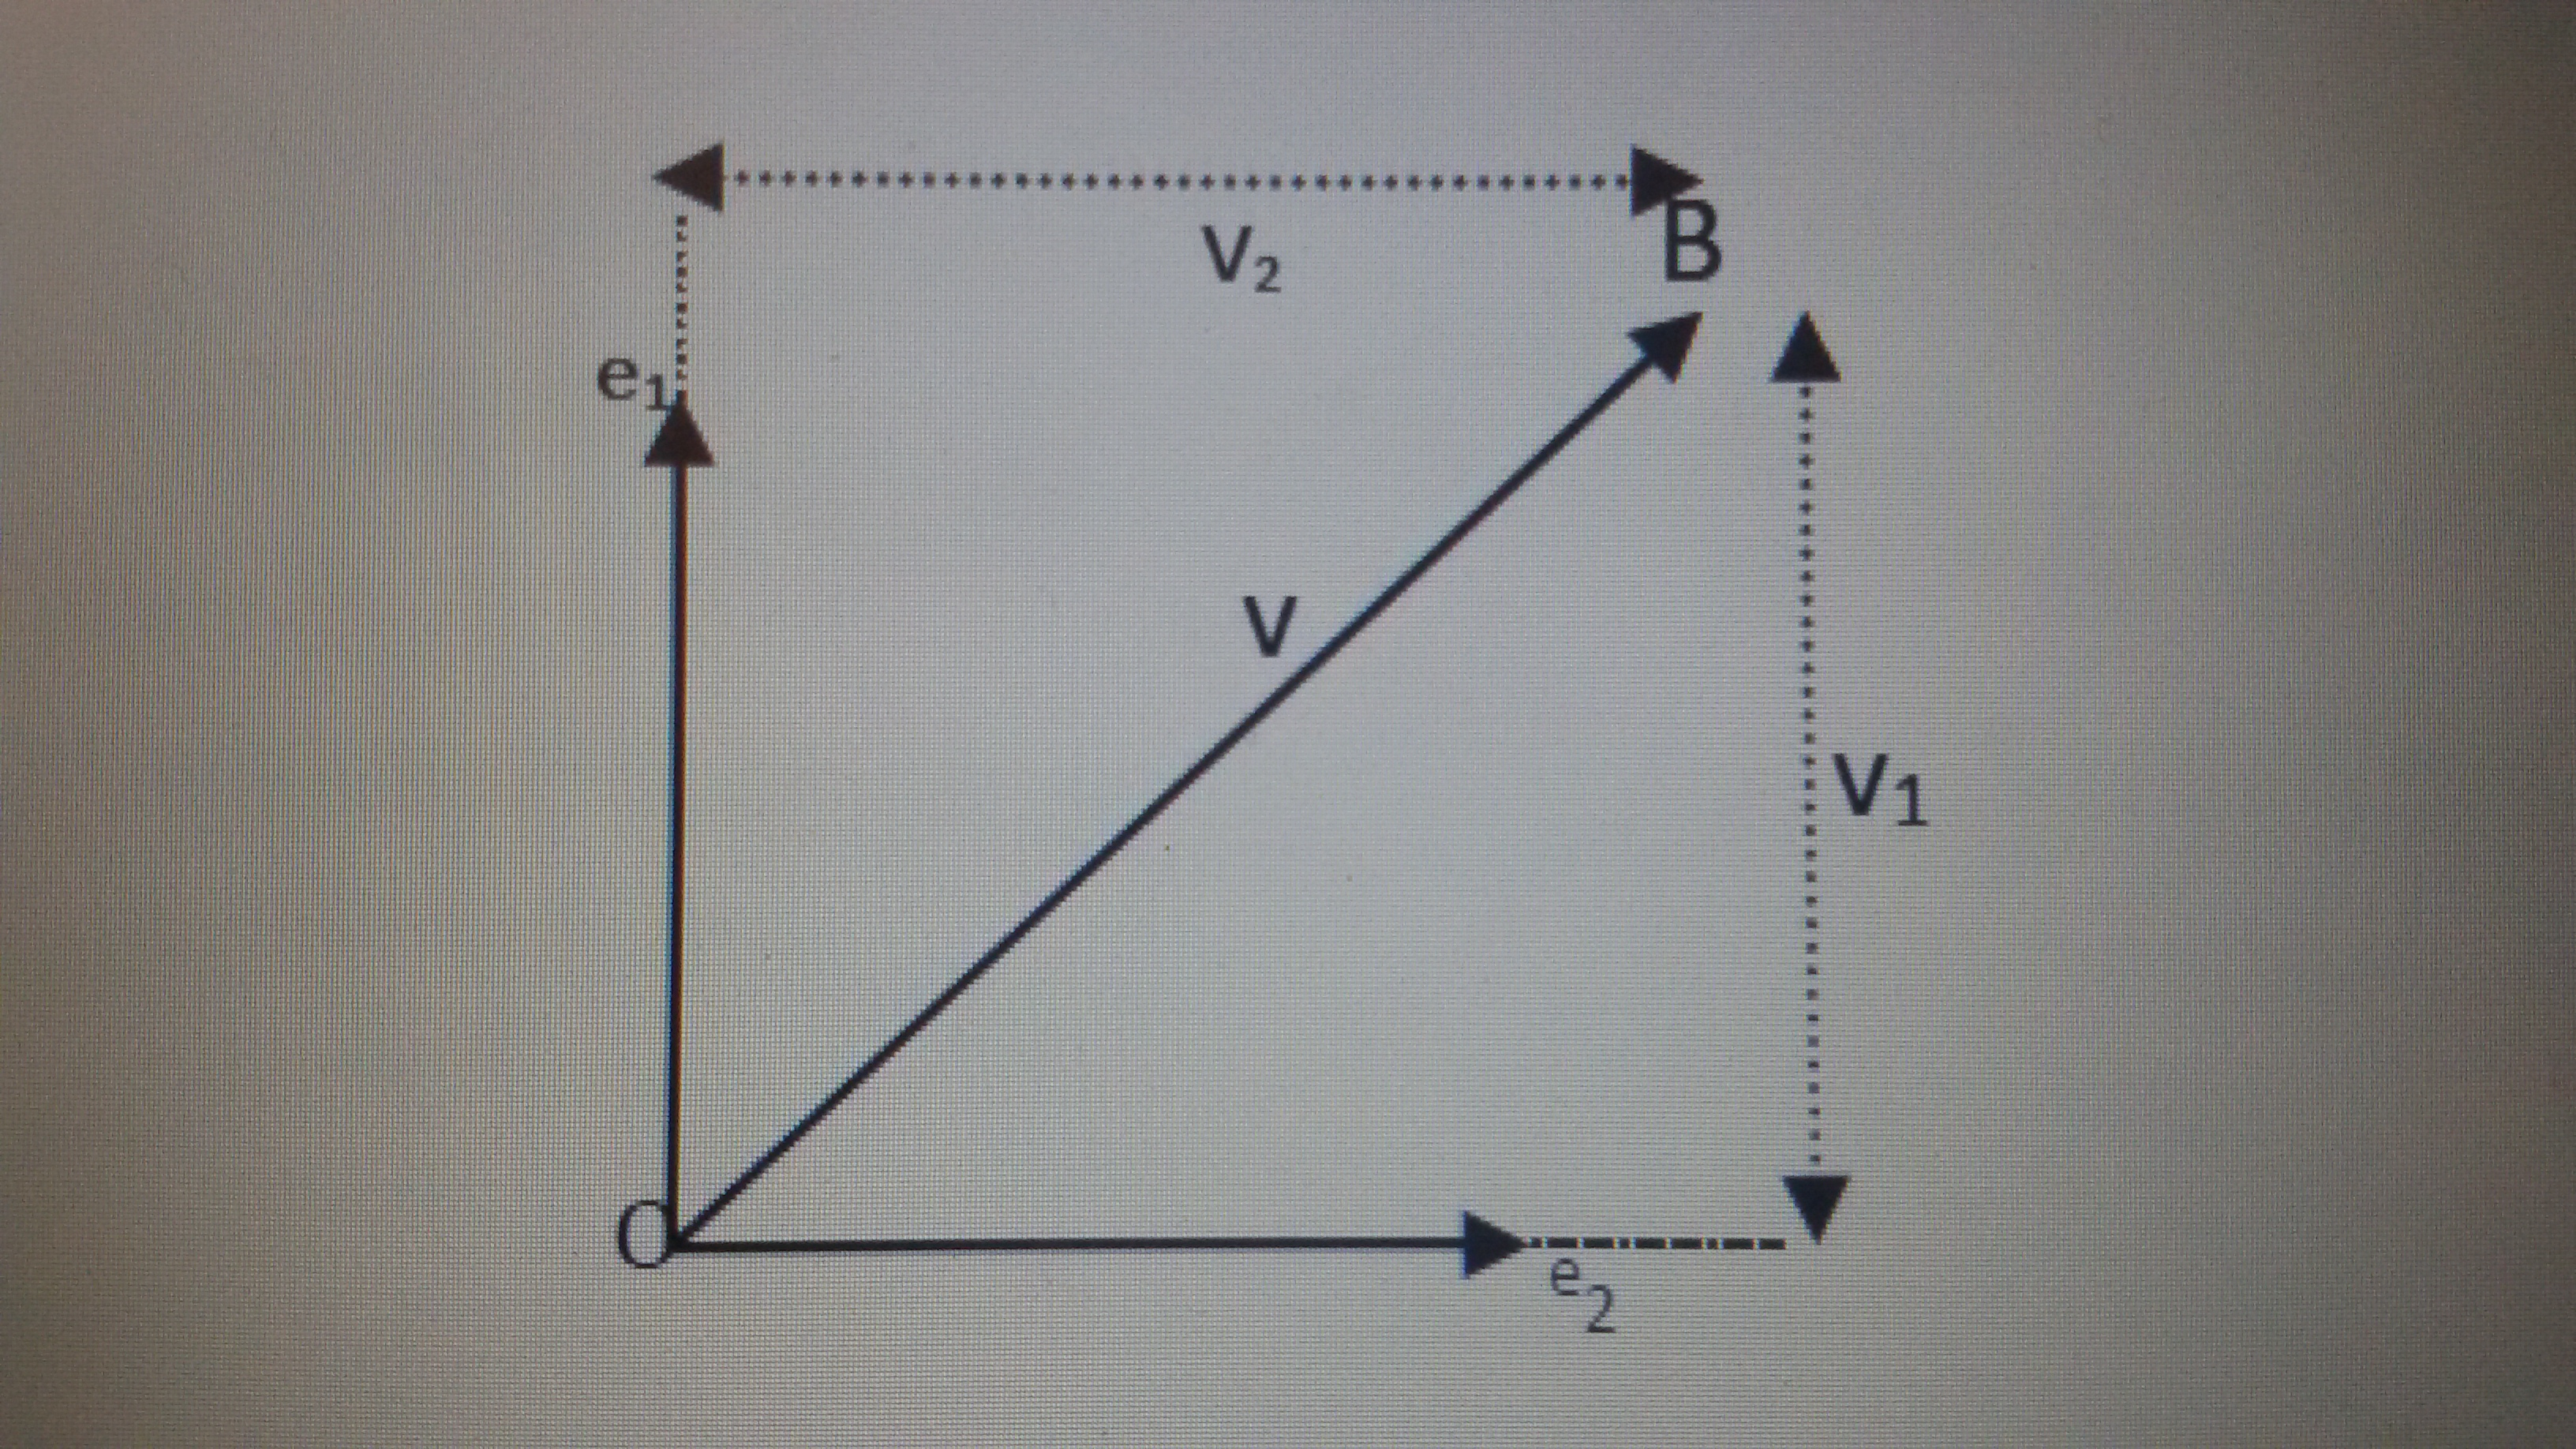
\includegraphics[scale=0.08]{figure.jpg}
\end{figure}
    
    
    Consider the above figure, here OB is a vector denoted by v which is expressed as
    \begin{equation*}v = v_1e_1 + v_2e_2\end{equation*}
    
    where $v_1$ and $v_2$ are the components in $e_1$ and $e_2$ directions respectively.
By this we can say that vectors $e_1$ and $e_2$ spans the space in 2D i.e. we can express any vector as a linear combination of e1 and e2. A collection of vectors span a space. Suppose if any vector can be expressed uniquely as a linear combination of $\{ u_1$,$u_2$,$u_3$ .... $u_n \}$, where $\{ u_1$,$u_2$,$u_3$...$u_n \}$ are linearly independent, then $\{ u_1$,$u_2$...$u_n \}$ is said to form a basis.\\
\noindent
Also, if $\langle u_i$,$u_j \rangle$ = 0 for i,j belonging from 1 to n,i.e. dot product of any two vectors is zero,  then the basis is said to be an \textit{orthogonal basis}. Finally, for a n-dimensional space, a collection of n linearly independent vectors forms the basis.\\
\noindent
The dot product of two vectors $u$ and $v$ is equal to the sum of the products of the corresponding perpendicular components. Suppose

				\begin{equation*}u = u_1e_1 + u_2e_2\end{equation*}
                        
                        \begin{equation*}v = v_1e_1 + v_2e_2\end{equation*} 
\noindent                        
                        therefore,\begin{equation*} u.v = u_1v_1 + u_2v_2\end{equation*}
           
\subsubsection{Dot Product of Discrete Sequences}           
Now, consider a discrete sequence with 2 non-zero points. This sequence can be compared to a 2-dimensional vector v with $v_1$ and $v_2$ as its perpendicular components such that it is equal to the values at the 2 non zero points of the sequence. Similarly for a sequence with n non-zero points can be considered as a vector in n dimensional space. Also, the concept of dot product is similarly applied to the discrete sequences.

For example : Consider
	x[n] = $(1/2)^n$ u[n];
    
    i.e.
     \begin{equation*}
    x[n] = (1/2)^n	\enspace	\enspace for\enspace	 n\geq0\end{equation*}
    \begin{equation*}	 0	\enspace  \enspace	 for\enspace	 n<0\end{equation*}
               
	 \begin{equation*} y[n] = (1/3)^nu[n] \end{equation*}
    
    i.e. 
    \begin{equation*}y[n] = (1/3)^n	\enspace \enspace	for\enspace n\geq0\end{equation*} \begin{equation*}0\enspace \enspace			for\enspace n<0 \end{equation*}
                  
                  
  Lets calculate the dot product of x[n] and y[n],i.e. summing the product of corresponding components.
  We have,
   \begin{equation*} \langle x[n],y[n] \rangle = \sum_{n=-\infty}^{\infty}\ x[n]y[n]\end{equation*} 
   \begin{equation*} \langle x[n],y[n] \rangle = \sum_{n=0}^{\infty}\ x[n]y[n]\end{equation*} 
   \begin{equation*} \langle x[n],y[n] \rangle = \sum_{n=0}^{\infty}\ (1/2)^n*(1/3)^n\end{equation*} 
   \begin{equation*} \langle x[n],y[n] \rangle = \sum_{n=0}^{\infty}\ (1/6)^n\end{equation*} 
   \begin{equation*} \langle x[n],y[n] \rangle = \frac{1}{(1-(1/6))}\end{equation*} 
   \begin{equation*} \langle x[n],y[n] \rangle = \frac{6}{5}\end{equation*} 
  		
          
 	By this we compute the dot product of two discrete sequences. This dot product is also called as \textit{Inner Product}. Inner product of two vectors $u$ and $v$ is represented by $\langle u,v \rangle$.

\subsubsection{Inner Product of Continuous Signals}
       In a discrete sequence, a unit vector can be expressed as $\delta[n-N]$ for all integers Z. A n-dimensional vector v can be expressed as
        \begin{equation*}v = v_1e_1 + v_2e_2 + ........ + v_ne_n\end{equation*}
        Now writing the above equation in terms of sequences, we have
       
    	\begin{equation*}	x[n] = 	\sum_{n=-\infty}^{\infty}\ x[N]\delta[n-N]\end{equation*}
            
            where x[n] is the component along dimension N.
       
Similarly applying the same concept for continuous time functions, we need to replace summation by integral, which gives,

					\begin{equation*}x(t) = \int_{-\infty}^{\infty} \! x(\lambda)\delta[t-\lambda] \ \mathrm{d}\lambda\end{equation*}
                    
             where x($\lambda$) is the component in direction $\lambda$ and $\delta[t-\lambda]$ is continuous impulse at $\lambda$ similar to unit vector.So inner product of x(t) and y(t) is given by
             
           \begin{equation*} \langle x(t),y(t) \rangle = \int_{-\infty}^{\infty} \! x(t)y(t) \ \mathrm{d} t\end{equation*}
             
 \subsection{Sinusoids with same period}
          Let us see how we can express any signal as sinusoidal functions. So, first we need to find sinusoidal signals which are perpendicular. Consider a signal x(t) which is periodic with period T,i.e. \begin{equation*}  x(t) = x(t+T)\end{equation*}. Assume that it can be expressed as a sum of sinusoidal functions. We should take a sinusoidal function which is periodic with period T. So it is of the form $A_k\cos (\frac{2\pi}{T}kt + \phi_k)$. We have,
          
          \begin{equation*}x(t) = \sum_{k=-\infty}^{\infty}\ A_k\cos (\frac{2\pi}{T}kt + \phi_k)\end{equation*}
          
          Let's take two different \textit{k}
.  \begin{equation*}
x_1 (t) = A_1 \cos (\frac{2\pi}{T}k_1t + \phi_1)
\end{equation*}
           and \begin{equation*}
x_2 (t) = A_2 \cos (\frac{2\pi}{T}k_2t + \phi_2)
\end{equation*}
          Consider the inner product of $x_1(t)$ and $x_2(t)$ with the interval going from 0 to T. We are here restricting our interval to T because the integral might diverge when we integrate from 0 to $\infty$. We have,
           \begin{equation*}\langle x_1(t),x_2(t) \rangle = \int_{0}^{T} \! x_1(t)x_2(t) \ \mathrm{d}t\end{equation*}
           \begin{equation*}\langle x_1 (t),x_2 (t) \rangle = \int_{0}^{T} \! \cos (\frac{2\pi}{T}k_1t + \phi_1) \cos (\frac{2\pi}{T}k_2t + \phi_2) \ \mathrm{d}t\end{equation*}
           Using 
          \begin{equation*} 2cosAcosB = cos(\frac{A+B}{2}) + cos(\frac{A-B}{2})\end{equation*}
          We have,
          \begin{equation*}\langle x_1 (t),x_2 (t) \rangle = \int_{0}^{T} \! \left\lbrace \cos (\frac{2\pi}{T}\frac{(k_1+k_2)}{2}t + \frac{\phi_1+\phi_2}{2}) + \cos (\frac{2\pi}{T}\frac{(k_1-k_2)}{2}t + \frac{\phi_1-\phi_2}{2}) \right\rbrace \ \mathrm{d}t \end{equation*}
          
          
        
        
                
                If ($k_1$ + $k_2$) or ($k_1$ - $k_2$) are not zero, that means we have a finite number of cycles of the sinusoids, implying the integral is zero. However if $k_1$=$k_2$, the second integral becomes T times $\cos (\theta_1-\theta_2)$.
                Thus we have,
            \begin{equation*} \langle x_1 (t),x_2 (t) \rangle  \neq 0	\enspace \enspace		for \enspace k_1 = k_2\end{equation*}
            \begin{equation*} \langle x_1 (t),x_2 (t) \rangle = 0	\enspace \enspace		for \enspace k_1 \neq k_2\end{equation*}
                
                
                Hence, we have proved that two sinusoids with same time period are perpendicular if they don't have same angular frequency and vice-versa. Thus using this important concept, we will be able to write any signal as sum of sinusoidal signals and hence analysis of these signals will be simpler.


\section{Module 2: Lecture 4\\Decomposition of Signals}

\subsection{Introduction}
\noindent
 A fundamental idea in the study of signals is to represent signals in terms of linear combination of \textit{basis} signals. In the previous section, we have embarked on some important concepts, relating to the idea of representing signals as a linear combination of sinusoids.
 %In this lecture, we will be recapitulating those ideas.
We assumed that we wish to look either at periodic signals or signals over a finite interval $T$. Without loss of generality, let that interval be $(0,T)$. 

\noindent
We have assumed that such signals are signals spanned by  all sinusoids of angular frequency $\Omega = \frac{2\pi}{T}kt,k=0, \pm1, \pm2 ..$

\noindent
The typical periodic function, with period $T$ is of the form
\begin{equation*}
  x(t) = \sum_{k=-\infty}^{\infty} \! A_k\cos (\frac{2\pi}{T}kt + \phi_k)
\end{equation*}
where $A_k$ denotes the amplitude, $\Omega = \frac{2\pi}{T}k$ is the angular frequency and $\phi_k$ the phase.
We had proved that these sinusoids are orthogonal if they don’t have same angular frequency.
\begin{equation*}
  \langle A_{k_1} \cos (\frac{2\pi}{T}k_1t + \phi_1),A_{k_2} \cos (\frac{2\pi}{T}k_2t + \phi_2)\rangle = 0 \enspace \enspace \text{for} \enspace k_1 \neq k_2 
\end{equation*}

\noindent
This important concept requires appreciating several different ideas. Using these ideas, we can decompose signal $x(t)$ in terms of sinusoids. However, there are some signals which can’t be spanned using these sinusoids. Such signals are beyond the scope of discussion that we are going to undertake at this stage.
%%%
%%%
\subsection{ Orthogonal vectors at a particular frequency}
\noindent
Consider a periodic signal $x(t)$ with fundamental period $T$. Then we can write $x(t)$ as
%Let us assume the signal $x(t)$ as
\begin{equation*}
  x(t) = \sum_{k=-\infty}^{\infty} \! A_k\cos (\frac{2\pi}{T}kt + \phi_k)
\end{equation*}
%where $x(t)$ is periodic with period $T$ and w
We constrain ourselves to $0<t<T$.

\noindent
To calculate $A_k$ and $\phi_k$ we need to use the following property i.e.
\begin{equation*}
\langle \cos (\frac{2\pi}{T}k_1t + \phi_1), \cos (\frac{2\pi}{T}k_2t + \phi_2) \rangle = 0 \enspace \enspace		for \enspace k_1 \neq k_2 \end{equation*}

\noindent
We can think of the cosines $\cos (\frac{2\pi}{T}kt + \phi_k)$ as countably infinite orthogonal vectors, indexed by $k$, for $k=0, \pm1, \pm2...$ and so on.

\noindent
To find out the component of $x(t)$ along these orthogonal vectors, we need to take the dot product of $x(t)$ with the unit vector, in the direction of orthogonal vectors $\cos(\frac{2\pi}{T}kt + \phi_k), 0<t<T$.
For calculating unit vector, we need to find the magnitude of the vector $\cos(\frac{2\pi}{T}kt + \phi_k)$ using dot product.

\begin{align*} \left|\cos(\frac{2\pi}{T}kt + \phi_k)\right| &= \langle \cos (\frac{2\pi}{T}kt + \phi_k), \cos (\frac{2\pi}{T}kt + \phi_k)\rangle \\
  &= \int_{0}^{T} \! \cos (\frac{2\pi}{T}kt + \phi_k) \cos (\frac{2\pi}{T}kt + \phi_k) \ \dm t \\
  &= \int_{0}^{T} \! \cos^2 (\frac{2\pi}{T}kt + \phi_k) \ \dm t \\
  &= \int_{0}^{T} \! (\frac{1}{2} + \cos (2(\frac{2\pi}{T}kt + \phi_k)) \ \dm t \\
  &= \int_{0}^{T} \! \frac{1}{2} \ \dm t + \int_{0}^{T} \! \cos (2(\frac{2\pi}{T}kt + \phi_k)) \ \dm t \\
  &= \frac{T}{2}
\end{align*}
%%%
Thus, the magnitude square of the cosine is $T/2$ and hence the magnitude is $\sqrt{T/2}$. So, the unit vector is given by

\begin{equation*} \textrm{Unit vector} = \sqrt{\frac{2}{T}}\cos (\frac{2\pi}{T}kt + \phi_k)\end{equation*}
                    
\noindent
But still, there is one unknown quantity, namely, $\phi_k$ in this unit vector. However, we can think of this vector as a vector in a two dimensional space:

\begin{equation*}\sqrt{\frac{2}{T}}\cos (\frac{2\pi}{T}kt + \phi_k) = \sqrt{\frac{2}{T}}[\cos\phi_k\cos (\frac{2\pi}{T}kt) - \sin\phi_k\sin (\frac{2\pi}{T}kt)] \end{equation*}
that is, the unit vector can be thought of as a linear combination of two vectors.

\noindent
We have,
\begin{align*}
  \langle \cos (\frac{2\pi}{T}kt + \phi_k), \sin (\frac{2\pi}{T}kt + \phi_k) \rangle &= \int_{0}^{T} \! \cos (\frac{2\pi}{T}kt + \phi_k) \sin (\frac{2\pi}{T}kt + \phi_k) \ \dm t  \\
  &= \frac{1}{2} \int_{0}^{T} \! 2 \cos (\frac{2\pi}{T}kt + \phi_k) \sin (\frac{2\pi}{T}kt + \phi_k) \ \dm t \\
  &= \frac{1}{2} \int_{0}^{T} \! \sin (\frac{4\pi}{T}kt + \phi_k) \ \dm t \\
  &= 0
\end{align*}
%%%
Hence, the cosine and sine components are also orthogonal. $\cos\phi_k$ and $\sin\phi_k$ are now two unknown constants.
%%%
Therefore, decomposing $x(t)$ along $\cos (\frac{2\pi}{T}kt + \phi_k)$ will give the same results as decomposing $x(t)$ along  $\cos (\frac{2\pi}{T}kt)$ and $\sin (\frac{2\pi}{T}kt)$. So, to decompose $x(t)$ along $\cos (\frac{2\pi}{T}kt)$ and $\sin (\frac{2\pi}{T}kt)$, we require unit vectors, which we already have calculated above.
%%%
So, the two unit vectors are $\sqrt{\frac{2}{T}}\cos (\frac{2\pi}{T}kt)$ and $\sqrt{\frac{2}{T}}\sin (\frac{2\pi}{T}kt)$.
%%%
%%% 
\subsection{Projection of Vectors}
Let $u_1$ = $\sqrt{\frac{2}{T}}\cos (\frac{2\pi}{T}kt)$ and $u_2 = \sqrt{\frac{2}{T}}\sin (\frac{2\pi}{T}kt)$. We know that at frequency $2\pi k/T$, there are two orthogonal vectors, $u_1$ and $u_2$. We have a two dimensional space and we need to calculate the component of the vector $x(t)$ along orthogonal vectors of this 2D space.
  
\noindent
 Let $v$ be any arbitrary vector of higher dimension and $v_p$ be the projection of $v$ onto our 2D space spanned by orthogonal vectors $u_1$ and $u_2$. To calculate the components of the vector $v$ along the two orthogonal vectors, we can project $v_p$  onto $u_1$ and $u_2$. We can also directly project $v$ onto $u_1$ and $u_2$.
 


\noindent
 The vector $v$ can be written as $v = v_p  + v_\perp$, where $v_p$ is the projection of $v$ on to 2D space and $v_\perp$ is component perpendicular to the 2D space . The projection of $v$ onto vectors $u_1$ and $u_2$ will be same as the projection of $v_p$  on those vectors, as the $v_\perp$ will not contribute in projection.
 
\begin{figure}[ht]
\centering
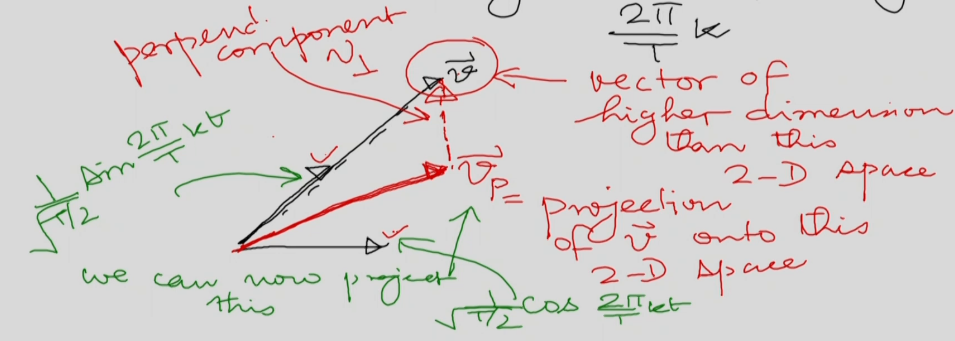
\includegraphics[scale=0.32]{S_215.PNG}		
\end{figure}

 \begin{figure}[ht]
\centering
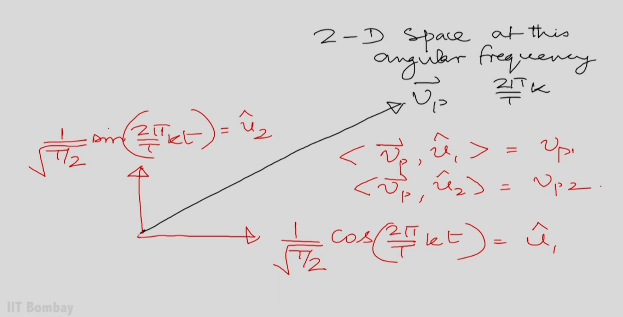
\includegraphics[scale=0.32]{S_215_2.PNG}		
\end{figure}

\noindent
Let us project $v_p$ along the two orthogonal vectors. 
  For projecting  $v_p$  along $u_1$ and $u_2$, taking dot product 
 
\begin{equation*} \langle v_p, u_1 \rangle =v_{p_1} \end{equation*}
\begin{equation*} \langle v_p, u_2 \rangle = v_{p_2} \end{equation*}
 
\noindent
$v_p$  in terms of $u_1$, $u_2$ can be written as $v_p$  = $v_{p_1}u_1$ + $v_{p_2}u_2$. Interestingly  $\langle v_p, u_1 \rangle = \langle v, u_1 \rangle$ is true also for $u_2$ as the perpendicular component $v_\perp$ is not going to contribute in the dot product. 
        
We know that the $k^{th}$ angular frequency =  $2 \pi k/T$.
At this frequency we have two components 
\begin{equation*}x(t) = \langle x(t), \sqrt{\frac{2}{T}}\cos (\frac{2\pi}{T}kt)\rangle \cdot \sqrt{\frac{2}{T}}\cos (\frac{2\pi}{T}kt) + \langle x(t), \sqrt{\frac{2}{T}}\sin (\frac{2\pi}{T}kt)\rangle \cdot \sqrt{\frac{2}{T}}\sin (\frac{2\pi}{T}kt)\end{equation*}
This can be simplified as

\begin{equation*}x(t) = \langle x(t), \cos (\frac{2\pi}{T}kt)\rangle \cdot \frac{2}{T}\cos (\frac{2\pi}{T}kt) + \langle x(t), \sin (\frac{2\pi}{T}kt)\rangle \cdot \frac{2}{T}\sin (\frac{2\pi}{T}kt)\end{equation*}

\noindent
\subsection{Decomposition of square wave}
We have a periodic signal $x(t)$ in Fig.\ref{fig:square-wave}, defined as
\[
x(t) =
\left\{
	\begin{array}{ll}
		1  & \mbox{if } 0 < t < \frac{T}{2} \\
		-1 & \mbox{if } \frac{T}{2} < t < T
	\end{array}
\right.
 \]

\noindent
$x(t) = x(t+T)$ for all $t$, i.e. $x(t)$ is periodic with period $T$.
              
\begin{figure}[ht]\label{fig:square-wave}
\centering
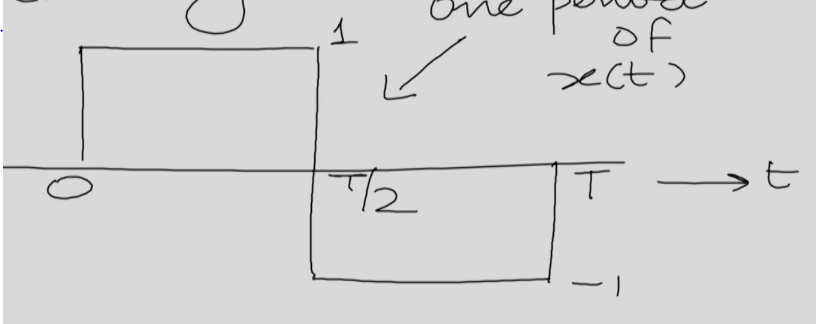
\includegraphics[scale=0.32]{S_216_1.PNG} %\\Figure 1
\caption{Plot of $x(t)$}
\end{figure}




\noindent
The zero frequency component is the  mean of $x(t)$ over a period $T$ which is $0$ since the net area under $x(t)$ in one period is zero.

\noindent
Let us calculate the quantity $\langle x(t), \cos (\frac{2\pi}{T}kt)\rangle \cdot \frac{2}{T}\cos (\frac{2\pi}{T}kt))$,


\noindent
For $k=1$ and $k=2$, we can see from Fig.\ref{fig:square-dot-cosine} that, the positive portion gets annulled by the negative portion. Similar is the case for $k=3, 4...$ and so on. Hence $\langle x(t), \cos (\frac{2\pi}{T}kt)\rangle= 0$ for given $x(t)$.


\begin{figure}[ht]\label{fig:square-dot-cosine}
\centering
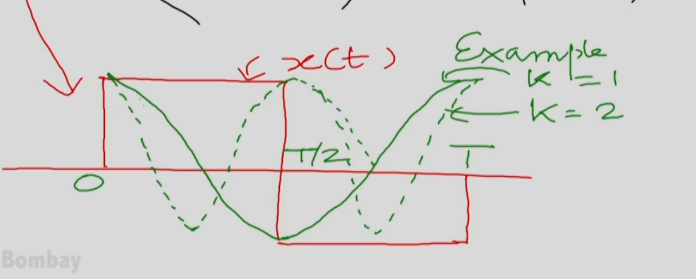
\includegraphics[scale=0.32]{s_216.PNG} %\\Figure 2
\caption{Dot product of the square wave with cosines}	
\end{figure}

\noindent
Calculating  $\langle x(t), \sin (\frac{2\pi}{T}kt)\rangle \cdot \frac{2}{T}\sin (\frac{2\pi}{T}kt)$, we have as shown in Fig.\ref{fig:square-dot-sine},

\begin{figure}[ht]\label{fig:square-dot-sine}
\centering
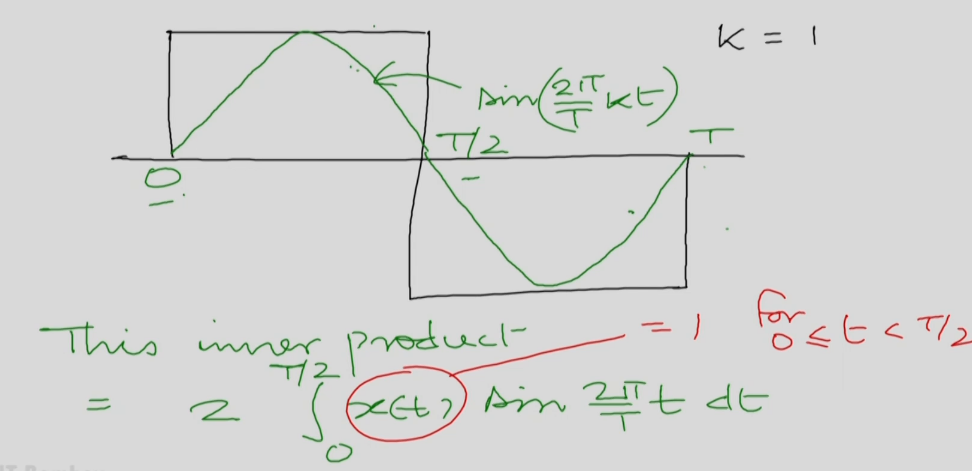
\includegraphics[scale=0.32]{S_216_3.PNG} %\\Figure 3
\caption{Dot product of the square wave with sines}	
\end{figure}
%%%
\begin{equation*} \langle x(t), \sin (\frac{2\pi}{T}kt)\rangle = \int_{0}^{T} \! x(t)\sin (\frac{2\pi}{T}kt) \ \dm t\end{equation*}
\begin{equation*} \langle x(t), \sin (\frac{2\pi}{T}kt)\rangle = \int_{0}^{\frac{T}{2}} \! \sin (\frac{2\pi}{T}kt) \ \dm t + \int_{\frac{T}{2}}^{T} \! {-\sin (\frac{2\pi}{T}kt)} \ \dm t \end{equation*}
\noindent
Also, we know that 
 \begin{equation*}\int_{0}^{\frac{T}{2}} \! \sin (\frac{2\pi}{T}kt) \ \dm t = -\int_{\frac{T}{2}}^{T} \! \sin (\frac{2\pi}{T}kt) \ \dm t \end{equation*}
\noindent
Using this, we have
\begin{equation*} \langle x(t), \sin (\frac{2\pi}{T}kt)\rangle = 2\int_{0}^{\frac{T}{2}} \! \sin (\frac{2\pi}{T}kt) \ \dm t = \left[-2\frac{\cos (\frac{2\pi}{T}kt)}{\frac{2\pi}{T}k}\right]_0^\frac{T}{2}\end{equation*}
%%%
For $k = 2n$, the above integral goes to zero as $\cos ({2\pi}n) = 1$ for all $n \in \mathbb{Z}$.
For $k = 2n-1$, the above integral has the value of $4T/\pi k$ because $\cos(2{\pi}(2n-1)) = -1$ for all $n \in \mathbb{Z}$. Thus,

\begin{equation*} \langle x(t), \sin (\frac{2\pi}{T}kt)\rangle = \frac{4T}{{\pi}k} \textrm{ (for odd }k) \end{equation*}
\noindent
Hence, we have, after multiplying by $2/T$,
\begin{equation*} x(t) = \sum_{n=1}^{\infty}\ \frac{4}{{\pi}(2k-1)} \sin (\frac{2\pi}{T}(2k-1)t)\end{equation*} 

\subsection{Examples of Decomposition}
\subsubsection{Exercise 1} 
\noindent
Work out the decomposition for an asymmetric square wave, of period $T$ as shown in the figure below.
\begin{figure}[ht]
\centering
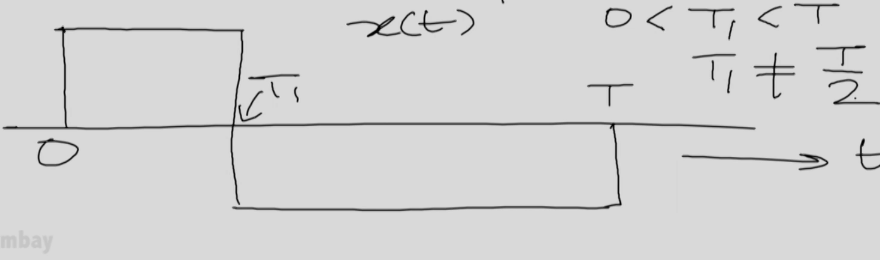
\includegraphics[scale=0.32]{S_217_1.PNG}
\end{figure}
 				\begin{equation*} x(t) = 1 \enspace \enspace      0<t<T_1 \end{equation*}
       			\begin{equation*} x(t) = -1  \enspace\enspace 	T_1 < t< T \end{equation*} \begin{equation*}0<T_1<T, \enspace T1\neq T/2, x(t+T) = x(t)\enspace  \forall t\in R.  \end{equation*}

                
\subsubsection{Exercise 2}
\noindent
In the answer of exercise 1 put $T_1 =T/2$, and verify the answer with that of decomposition of symmetric square wave.

\subsubsection{Exercise 3}
\noindent
Work out the decomposition for symmetric triangular wave, periodic with period $T$.

\noindent
\textit{Hint}: Use and observe the symmetry graphically.
\begin{figure}[ht]
\centering
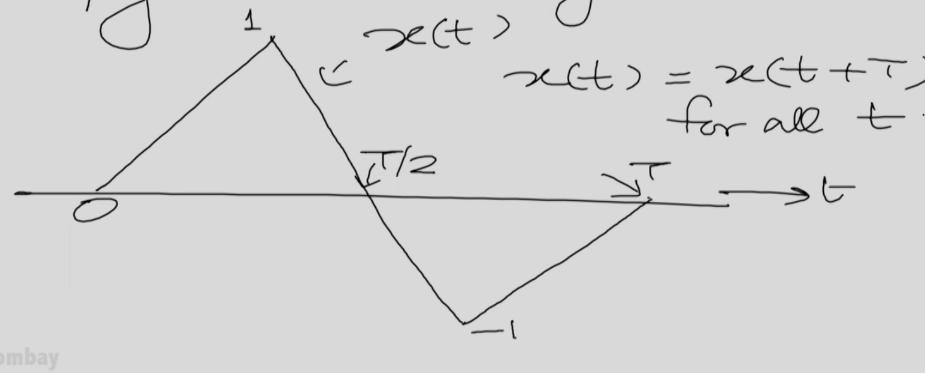
\includegraphics[scale=0.32]{S_217_2.PNG}
\end{figure}


\subsubsection{Exercise 4}
\noindent
Evaluate the decomposition for an asymmetric triangular wave as shown in the figure. Cross check the answer with that of exercise 3, by putting  $T_1 = T/2$ in the final answer.
\begin{figure}[ht]
\centering
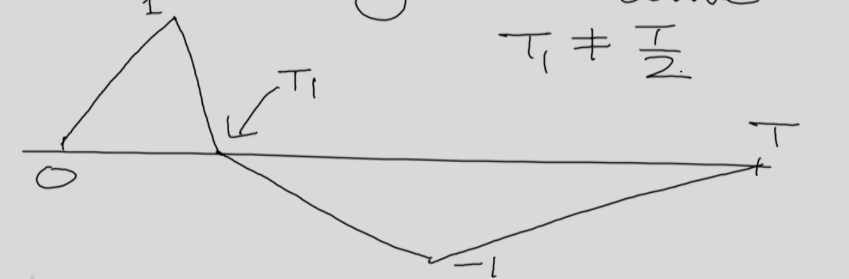
\includegraphics[scale=0.32]{S_217_3.PNG}
\end{figure}


\subsubsection{Exercise 5}
\noindent
A variant of symmetric triangular wave is shown below. Find its decomposition and compare with answer of exercise 3.
\begin{figure}[ht]
\centering
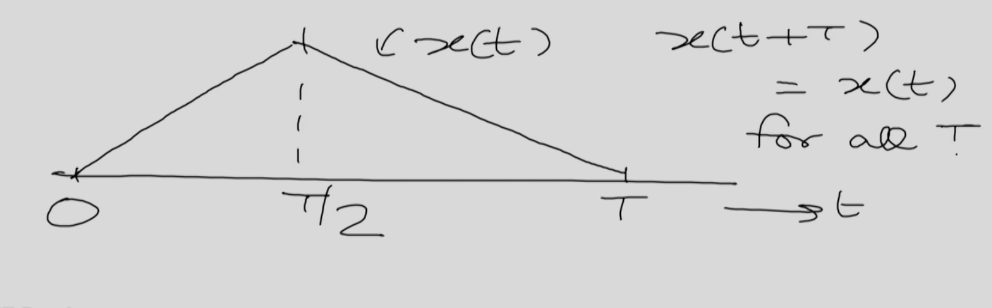
\includegraphics[scale=0.32]{S_217_4.PNG}
\end{figure}

\pagebreak

\subsubsection{Exercise 6}
\noindent
A variant of an asymmetric triangular wave is shown below. Evaluate the decomposition of  this wave. Substitute $T_1 = T/2$, in the answer and compare with the result of exercise 5. Explain the differences in the result, if any.
\begin{figure}[ht]
\centering
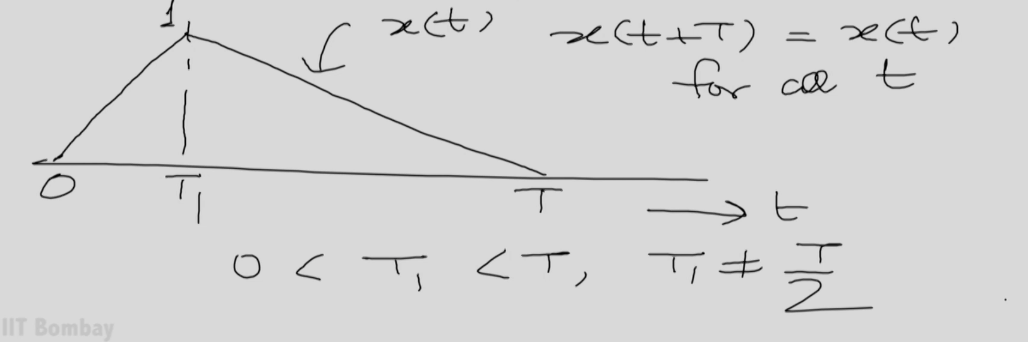
\includegraphics[scale=0.32]{S_217_5.PNG}
\end{figure}








                



                     

\section{Module 2: Lecture 5\\Fourier Series Decomposition and its Applications}

\subsection{Introduction}
We have been decomposing periodic waveform into their periodic sinusoidal components. In this lecture we look at a variation of the same decomposition using complex exponential functions. One way of doing this is to convert each sinusoidal component of sinusoidal decomposition into corresponding exponential functions. However, in some cases, we prefer to a priori decompose the waveform in complex exponential components.
\newline
We shall also see how to go from the complex exponential components to sinusoidal components. We will then look at the applications of both sinusoidal and complex exponential decompositions; in particular, we will be analyzing its utility in determining the output from a linear shift invariant system on applying a periodic input.
We will also see some conditions under which we cannot obtain a Fourier series decomposition for a periodic waveform.

\subsection{Complex Exponential Fourier Series Decomposition}
Suppose we are given a periodic signal $x(t)$ with period $T$. We wish to write $x(t)$ in terms of sum of complex exponential functions:
$$ x(t) = \sum_{k=-\infty}^{\infty}{C_{k} \ e^{j2\pi kt/T}} $$
where $C_k$ belongs to the set of complex numbers.
Basically, we are trying to write $x(t)$ as a linear combination complex exponential functions rotating at angular frequencies $2\pi k/T$ for all integer $k$. Notice that complex exponentials with angular frequencies as positive integral multiples of $2\pi kt/T$ represent anticlockwise rotating phasors while the complex exponentials with negative angular frequencies represent clockwise rotating phasors.
\newline
\subsubsection{Orthogonality of Fourier Series Components}
We now establish orthogonality between the complex exponential components.
We take 2 integers $k$ and $l$ and evaluate the inner product
\begin{equation}
\int_{-T/2}^{T/2}{\frac{1}{T}e^{(j2\pi kt/T)}e^{(j2\pi (-l)t/T)}}dt = \int_{-T/2}^{T/2}{\frac{1}{T}e^{(j2\pi (k-l)t/T)}}dt
\end{equation}
We have 2 cases now:
\begin{itemize}
\item {\textbf{Case 1}} $k=l$ The integral in (1) becomes $\int_{-T/2}^{T/2}\frac{1}{T}dt = 1$
\item {\textbf{Case 2}} $k \neq l$ The integral in (1) becomes $$\int_{-T/2}^{T/2}{\frac{1}{T}e^{(j2\pi (k-l)t/T)}}dt = \frac{1}{T}\frac{e^{(j2\pi (k-l)t/T)}}{(j2\pi (k-l)/T)}\Bigg|_{-T/2}^{T/2} = 0$$
\end{itemize}
\subsubsection{Obtaining Complex exponential Decomposition from Sinusoidal Decomposition}
Suppose we are given the sinusoidal components of the decomposition of a real waveform $$x(t) = \sum_{0}^{\infty}A_{k}\cos(2\pi kt/T + \phi_{k})$$
Note that in the above sum, for $k = 0$, we will have the component as $A_{0}\cos(\phi_{0})$, we can merge constant $\cos(\phi_{0})$ into $A_{0}$ and we will simply have constant $A_{0}$ for $k = 0$.
Now for a non-zero integer $k$ using $\cos(\theta) = \frac{1}{2}(e^{j\theta} + (e^{j\theta})^{*})$, (Note: $C^{*}$ denotes complex conjugate of $C$), we have $$A_{k}\cos(2\pi kt/T + \phi_{k}) = \frac{1}{2}\Bigg(A_{k}e^{j\phi_{k}}e^{j2\pi kt/T} + (A_{k}e^{j\phi_{k}})^{*} (e^{-j2\pi kt/T})\Bigg)$$
since $A_k$ are real.
$$\implies C_{k} = \frac{1}{2}A_{k}e^{j\phi_{k}}$$
$$\implies C_{-k} = \frac{1}{2}(A_{k}e^{j\phi_{k}})^{*}$$
And we also have trivially $C_{0} = A_{0}$
Notice that for real waveform, we have $C_{k} = (C_{-k})^{*}$


\subsubsection{Converting Complex Exponential to Sinusoidal Decomposition}
Suppose we are given a real $$ x(t) = \sum_{k=1}^{\infty}{C_{k}e^{(j2\pi kt/T)}} + \sum_{k=-\infty}^{-1}{C_{k}e^{(j2\pi kt/T)}} + C_{0}$$
Now, note that for an integer $k \neq 0$, $$\int_{-T/2}^{T/2}e^{(j2\pi kt/T)}dt = \frac{1}{T}\frac{e^{(j2\pi kt/T)}}{(j2\pi k/T)}\Bigg|_{-T/2}^{T/2} = 0$$
whereas, for k = 0, $$\int_{-T/2}^{T/2}1dt = T$$
So, basically we can obtain $C_{0}$ by integrating $x(t)$ over time $T$. In the Fourier Decomposition only $C_{0}$ will give a non zero integral which is equal to $C_{0}\cdot T$
Hence, $$C_{0} = \frac{1}{T}\int_{-T/2}^{T/2}x(t)dt$$
Now, since for real $x(t)$ we have $C_{k} = (C_{-k})^{*}$, we get
$$C_{k}e^{j2\pi kt/T} = (C_{-k}e^{-j2\pi kt/T})^{*}$$ So we have $$C_{k}e^{j2\pi kt/T} + C_{-k}e^{-j2\pi kt/T} = 2 Re (C_{k}e^{j2\pi kt/T})$$
Using the polar form of $C_{k}$ which is $|{C_{k}}|e^\phi_{k}$, we get
$$ 2 Re (C_{k}e^{j2\pi kt/T}) =  2|{C_{k}}|Re(e^{j2\pi kt/T + \phi_{k}} = 2|{C_{k}}|\cos(j2\pi kt/T + \phi_{k})$$
Finally, we have the sinusoidal decomposition
$$x(t) = C_{0} + \sum_{k=1}^{\infty}2|{C_{k}}|\cos(j2\pi kt/T + \phi_{k})$$

\subsection{Periodic Input to a Simple RC Circuit}

Suppose, we apply a real periodic voltage waveform $x(t)$ as input to a series RC-circuit with time period $T$. Recall that an RC circuit is a linear shift invariant system. Suppose we can write complex exponential decomposition of $x(t)$ as $$\sum_{k=-\infty}^{\infty}{C_{k}e^{(j2\pi kt/T)}}$$ The advantage of doing this is that we can use the fact that a complex exponential input to a linear shift invariant system simply gives the same complex exponential multiplied by a constant as its ouput. By phasor analysis of the circuit, we have the transfer function $$ \frac{j(2\pi k/T) CR}{1 + j(2\pi k/T) CR}$$
So, the output waveform will be simply $$y(t) = \sum_{k=-\infty}^{\infty} \frac{j(2\pi k/T) CR}{1 + j(2\pi k/T) CR} {C_{k}e^{(j2\pi kt/T)}}$$


This illustrates the power of having complex exponential decomposition of a waveform since we can obtain the output waveform quite simply if it is passed through a linear shift invariant system. Now, one catch in the above discussion is that we assumed that the decomposition of $x(t)$ in to a Fourier series is possible. It turns out it's \emph{not} always the case that we can write a Fourier series decomposition for a periodic waveform! Although, for most of the practical waveforms, we can write it. We will look at the conditions under which we can write the Fourier series decomposition for a periodic waveform. There are some waveforms for which we cannot find the Fourier decomposition. One such example is $x(t) = \sin{(1/frac(t))}$ where $frac(t)$ denotes fractional part of $t$. So, $x(t)$ is periodic with period 1 but still its Fourier series decomposition fails to exist. There are certain conditions under which Fourier analysis can be done, they are called the ‘Dirichlet’ Conditions. We shall not discuss them here.


\subsection{Periodic Inputs to a General Linear Shift Invariant System}

In this section we use Fourier series decomposition to determine output from a linear shift invariant system on applying a periodic input waveform. Of course for our analysis, will assume that Fourier series decomposition of the input waveform exists.
\newline
Let $\mathbb{S}$ denote a linear shift invariant system, let $h(t)$ be its impulse response. We apply a periodic input waveform $x(t)$. Now, using linearity of the system, output of the system is simply the sum of output obtained for each component of Fourier series decomposition of $x(t)$.
\newline
Let us derive the output for the $k^{\textnormal{th}}$ component of $x(t)$. The output for $k^{\textnormal{th}}$ will be the convolution of $h(t)$ and the input itself 
	$$\int_{-\infty}^{\infty}{h(\tau) \cdot C_{k}e^{j2\pi k(t- \tau)/T}}d \tau$$ Since, the above integral runs over $\tau$ and not $t$, the above expression reduces to 
    $$C_{k}e^{j2\pi kt/T}\int_{-\infty}^{\infty}{h(\tau) \cdot e^{-j2\pi k\tau/T}} d \tau$$
The integral reduces to a constant depending on k. So, what we obtain is quite interesting as it is simply the input itself multiplied by a constant!
Let us denote the constant by $\mathcal{H}(k)$. So, the output which is the sum of the outputs obtained for each component is
$$\sum_{k=-\infty}^{\infty}\mathcal{H}(k)C_{k}e^{j2\pi kt/T}$$

\subsection {Conclusion} In this lecture we discussed about Fourier series decomposition, its properties and its application in analysing linear shift invariant systems. In the coming lectures, we will discuss the significance of the quantity $\mathcal{H}(k)$ we derived in previous section and begin with what is known as Fourier Transform.







\chapter{The Fourier Transform}
\section{Module 2: Lecture 6\\The Fourier Transform}

\subsection{Introduction}
We are now in a position where we can deal with more general signals from the point of view of decomposition into sinusoidal frequency components and analysis as to what happens when you pass them through a linear shift invariant system. To do that, let's recapitulate some of the important conclusions that we had drawn in the previous chapter which will now help us in generalization.
%%%
%%%
\subsection{Recapitulation}
Let $\mathbb{S}$ be a linear shift invariant system with impulse response $h(t)$, and to it, we give a periodic signal input. Let’s assume that the Dirichlet conditions are obeyed. So we could decompose this into its Fourier series.
\begin{equation*}
x(t)= \sum\limits_{k=-\infty}^{k=+\infty}c(k)e^{j\Omega kt}
\end{equation*}
Where $\Omega=2\pi /T$ is the angular frequency and $c(k)$ are the Fourier coefficients. Now, the output can also be written as a Fourier series.
\begin{equation*}
y(t)= \sum\limits_{k=-\infty}^{k=+\infty}c(k)H(k\Omega)e^{j\Omega kt}
\end{equation*}
where
\begin{equation*}
H(\Omega)= \int_{-\infty}^{+\infty} \! h(t)e^{-j\Omega t} \ \dm t
\end{equation*}
%%%
%%%
\subsection{Interpretation of $H(\Omega)$ as a Dot Product}
We can interpret $H(\Omega)$ as a dot product or inner product. It’s an inner product between the impulse response $h(t)$ and the rotating phasor $e^{j\Omega t}$. An inner product with a unit vector calculates the projection or a component of the vector along the unit vector. So it's as if we are trying to find the component of the impulse response along a rotating phasor, rotating with an angular velocity $\Omega$. And, at the specific values of $\Omega$ given by each of the Fourier series components, we evaluate this dot product and use it to modify the Fourier series coefficient.
We can see from the equation of output $y(t)$ that output Fourier series coefficients are $c(k)H(\Omega k)$. Recall that in the input, the Fourier series coefficients were calculated by taking an inner product taking only one period of the input for the integral.
We took only one period of the input, and found the inner product with the corresponding harmonic or the complex exponential rotating with that particular multiple of the fundamental frequency. This is how we calculate the Fourier series coefficients.\\
Now, we can see that the Fourier coefficients of the output are the \emph{component by component multiplication of the Fourier coefficients of the input and impulse response}.
\[
Y(k\Omega)= c(k)H(k\Omega)
\]
Now, there are two questions to answer here. Here we have assumed that the input was periodic. What if it is not? Can we generalize this to a non-periodic function is a question that we need to answer. Secondly, can we think of this quantity $H(\Omega)$ as a new transform or a new way of dealing with the impulse response in its own right?\\
Now, a transform will make sense or will be adequate only if it is invertible. That is to say, we should be able to get back $h(t)$ from $H(\Omega)$. There should be no loss of information. It turns out that this is indeed the case. We can call $H(\Omega)$, for any $\Omega \in \mathbb{R}$, as the \emph{Fourier transform} of the impulse response $h(t)$.\\
Now let's try to address the question as to how can we \emph{go back} to $h(t)$ from $H(\Omega)$.
%%%
%%%
\subsection{Inverse for the Fourier Transform}
The answer to the question again lies in vector intuition. As we have seen, $H(\Omega)$ is the component of $h(t)$ along the phasor $e^{j\Omega t}$ for all such $\Omega \in \mathbb{R}$. In vector algebra, we get back a vector from its components by multiplying the components with their corresponding unit vectors and summing them. So, if $\hat{u}_1$ and $\hat{u}_2$ are two orthogonal unit vectors in two dimensions, $\overrightarrow{v}$ is a 2-D vector, and
\[
\langle \overrightarrow{v},\hat{u}_1 \rangle = v_1, \langle \overrightarrow{v},\hat{u}_2 \rangle = v_2
\]
Then, we construct $\overrightarrow{v}$ by multiplying the components with the corresponding unit vector and summing them. Hence
\[
\overrightarrow{v} = v_1\hat{u}_1 + v_2\hat{u}_2
\]
Now using the same principle here, $H(\Omega)$ are the components of the ``vector'' $h(t)$ along the unit vectors $e^{j\Omega t}$. Hence, to obtain the vector $h(t)$ back, we should multiply the component by the unit vector and sum up, or in this case, integrate over all $\Omega$.\\
But there are two subtleties involved here. Firstly, we don't know whether in this vector space of integrable functions, the vector $e^{j\Omega t}$ is a unit vector or not. That is, whether its magnitude is one or not. In case it is not one, we have to multiply it by a suitable constant to make it a unit vector. Secondly, we don't know whether $e^{j\Omega_1 t}$ and $e^{j\Omega_2 t}$ are orthogonal or not, for $\Omega_1 \neq \Omega_2$.\\
In the following subsection, we proceed to evaluate the inverse of $H(\Omega)$ assuming two things; one is that the vectors $e^{j\Omega t}$ are orthogonal, and that the multiplying factor $\kappa_0$ (for making it a unit vector) is independent of $\Omega$.
%%%
%%%
\subsubsection{Finding the Inverse of the Fourier Transform}
Form the previous discussion, the quantity we propose to be the inverse of $H(\Omega)$ is given by
\[
I = \int_{-\infty}^{\infty} \! H(\Omega)\ \kappa_0 e^{j\Omega t} \ \dm \Omega
\]
Now, we know that
\[
H(\Omega)= \int_{-\infty}^{\infty} \! h(t_1)e^{-j\Omega t_1} \ \dm t_1
\]
Putting this in $I$, we get,
\[
I = \int_{-\infty}^{\infty} \! \int_{-\infty}^{\infty} \! h(t_1)e^{-j\Omega t_1}\ \dm t_1 \ \kappa_0 e^{j\Omega t} \ \dm \Omega
\]
\[
= \int_{-\infty}^{\infty} \! h(t_1) \left\lbrace \int_{-\infty}^{\infty} \! \kappa_0 e^{-j\Omega t_1} \  e^{j\Omega t} \ \dm \Omega \right\rbrace \dm t_1
\]
Let's evaluate the quantity in the braces. We can write it as
\[
\lim_{\Omega_1 \to \infty} \int_{-\Omega_1}^{+\Omega_1} \! \kappa_0 e^{j\Omega (t-t_1)} \ \mathrm{d}\Omega
\]

\[
= \lim_{\Omega_1 \to \infty} \kappa_0 \frac{e^{j\Omega_1 (t-t_1)}-e^{-j\Omega (t-t_1)}}{j(t-t_1)}
\]

\[
= \lim_{\Omega_1 \to \infty}\frac{2\kappa_0 j\sin(\Omega_1 (t-t_1))}{j(t-t_1)}
\]

\[
= \lim_{\Omega_1 \to \infty}\frac{2\kappa_0\Omega_1\sin(\Omega_1 (t-t_1))}{\Omega_1(t-t_1)}
\]

Now, this can be written as 
\[
\lim_{\Omega_1 \to \infty} 2\kappa_0\Omega_1 \frac{\sin(x)}{x}
\]
where $x=\Omega_1(t-t_1)$. Now, $\sin(x)/x$ is not defined at $x=0$ as it has a zero divided by zero form. So we evaluate the limit as $x\to 0$.
\[
\lim_{x \to 0}\frac{\sin(x)}{x} = \lim_{x \to 0}\frac{\cos(x)}{1} = 1
\]
where the first equality is due to L'H\^opital's rule. This function will be oscillatory due to $\sin(x)$, but will decay as $x$ increases, due to the $x$ in the denominator. Also, the function will be zero when $x=n\pi$ or $\Omega_1(t-t_1)=n\pi$. Now, let's deal with this function as a function of $(t-t_1)$ rather than $x$. Let us try to plot the function
\[
f(t-t_1) = \frac{2\kappa_0\Omega_1\sin(\Omega_1 (t-t_1))}{\Omega_1(t-t_1)}
\]
The value of $\sin(x)/x$ is $1$ as $x \to 0$ as we saw earlier. Hence $f(0)=2\kappa_0\Omega_1$. Also the first null of the function will occur at $\Omega_1(t-t_1)=\pi$ or $(t-t_1)=\pi/\Omega_1$. Also the function is even with respect to $(t-t_1)$.
\begin{figure}[ht]
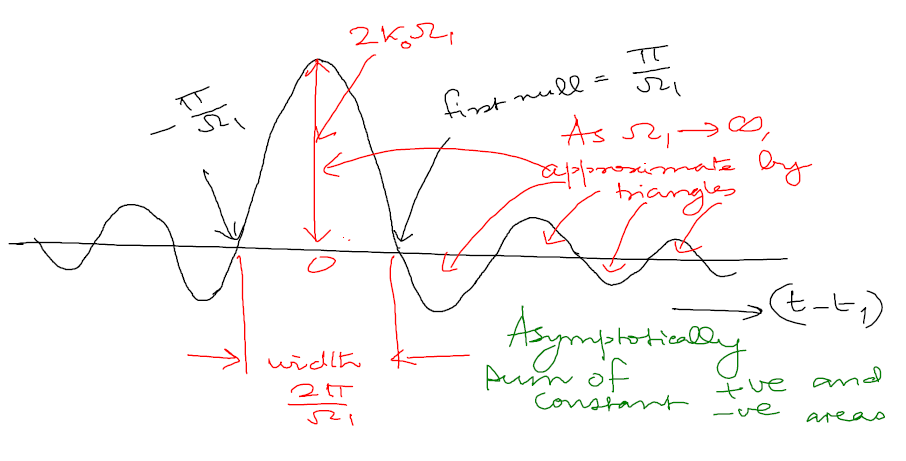
\includegraphics[scale=0.6]{fig.png}
\label{fig:sinc}
\caption{Sinc function}
\end{figure}
Hence, we will get a plot roughly as shown in Fig.\ref{fig:sinc}.
Now, we have to look at what happens when $\Omega_1 \to \infty$. We can see that the height of the main lobe at $x=0$ goes to infinity, but the width of the lobe, which is $2\pi/\Omega_1$ goes to zero, as $\Omega_1 \to \infty$. It can also be shown that the area of the other smaller lobes add up to zero, due to their alternating nature. Hence, we have a \emph{pulse} whose height is tending to infinity and the width to zero. In that case, we can assume the central lobe to be a triangle. Hence its area will be
\[
A = \frac{1}{2}\frac{2\pi}{\Omega_1}2\kappa_0\Omega_1 = 2\pi\kappa_0
\]
Hence, we can see that this area is a constant independent of $\Omega_1$. So we have a pulse having infinite magnitude and zero width, with a constant area encapsulated by it, and as you will remember from Part 1, this is nothing but the \emph{impulse function} $2\pi\kappa_0\delta(t-t_1)$.\\
Now, going back to our integral $I$,
\[
I = \int_{-\infty}^{\infty} \! h(t_1) \left\lbrace \int_{-\infty}^{+\infty} \! \kappa_0 e^{-j\Omega t_1} \  e^{j\Omega t} \ \mathrm{d}\Omega \right\rbrace \mathrm{d}t_1
\]
And we have evaluated the quantity in the braces to be $2\pi\kappa_0\delta(t-t_1)$. Hence,
\[
I = \int_{-\infty}^{\infty} \! h(t_1)\left\lbrace 2\pi\kappa_0\delta(t-t_1) \right\rbrace \mathrm{d}t_1 = 2\pi\kappa_0 \int_{-\infty}^{\infty} \! h(t_1) \delta(t-t_1)\ \mathrm{d}t_1
\]
Hence, by the sifting property of the delta function, we have,
\[
I = 2\pi\kappa_0 h(t)
\]
Hence, we can now set the value of $\kappa_0$ such that $I = h(t)$ as required. Hence $\kappa_0 = 1/2\pi$.\\
Hence, we finally have our expression for the \emph{Inverse Fourier transform} of $H(\Omega)$.
\[
h(t) = \frac{1}{2\pi}\int_{-\infty}^{\infty} \! H(\Omega)\  e^{j\Omega t} \ \mathrm{d}\Omega
\]
%%%
%%%
\subsection{Orthogonality of the Complex Exponentials}
A valid question to ask here is where did the orthogonality of the complex exponentials come in the picture. The answer lies in the integral in the braces which we evaluated.
\[
\int_{-\infty}^{+\infty} \! \kappa_0 e^{-j\Omega t_1} \  e^{j\Omega t} \ \mathrm{d}\Omega = 2\pi\kappa_0 \delta(t-t_1)
\]
or,
\[
\int_{-\infty}^{+\infty} \! e^{j\Omega t} \ \overline{e^{j\Omega t_1}} \ \mathrm{d}\Omega = 2\pi \delta(t-t_1)
\]
where the bar indicates complex conjugate. Now, this can be also written by renaming the variables, treating $t$ as the independent variable, as
\[
\int_{-\infty}^{+\infty} \! e^{j\Omega_1 t} \ \overline{e^{j\Omega_2 t}} \ \mathrm{d}t = 2\pi \delta(\Omega_1-\Omega_2)
\]
Now, we can immediately see that this is like an inner product between phasors rotating with different frequencies $\Omega_1$ and $\Omega_2$, and what this statement says is that it is non zero only for $\Omega_1=\Omega_2$. Hence, we do have some sense of orthogonality here. But since the value is infinite when the frequencies are equal, we have to call this a generalized orthogonality relation.
%%%
%%%
\subsection {Implications} 
Let's try to find what the Fourier transform expression implies. We have a non-periodic function $h(t)$ and we have decomposed it in its Fourier coefficients, not for discrete, but continuous set of frequency values, from minus to plus infinity. This can be thought of in the following way: We think of a non-periodic function as a periodic function with period tending to infinity. This is a valid statement, because as a periodic with period $T$ repeats itself after an interval $T$, we can say that a non-periodic function repeats itself after $T \to \infty$. Now, as the time period increases, the spacing between two adjacent frequencies decreases. And
\[
f = \lim_{T\to\infty}\frac{2\pi}{T} = 0.
\]
Hence, for a non-periodic function, the spacing between the adjacent frequencies tends to zero, which amounts to the Fourier spectrum going to continuous from discrete. This is exactly what has happened. The Fourier transform $H(\Omega)$ is a continuous function, and in general has a non-zero value for all $\Omega \in \mathbb{R}$.






\section{Module 2: Lecture 7\\Fourier Transforms properties and Fourier series example}

\subsection{Introduction}
	In this section, we will take a few examples of the calculation of the Fourier transform and then build upon the general properties of a Fourier transform like linearity, time shift, modulation and convolution. \\
	Let us start with calculating the Fourier transform of a rectangular pulse.
\subsection{Fourier transform of a Rectangular Pulse}
	Let the pulse be symmetric, with height equal to $A$, going from $-T/2$ to $T/2$ on the time axis. We call this function $h(t)$ as shown in Fig.\ref{fig:rectangular_pulse}.
	%%%
	\begin{figure}[htp]
		\centering
		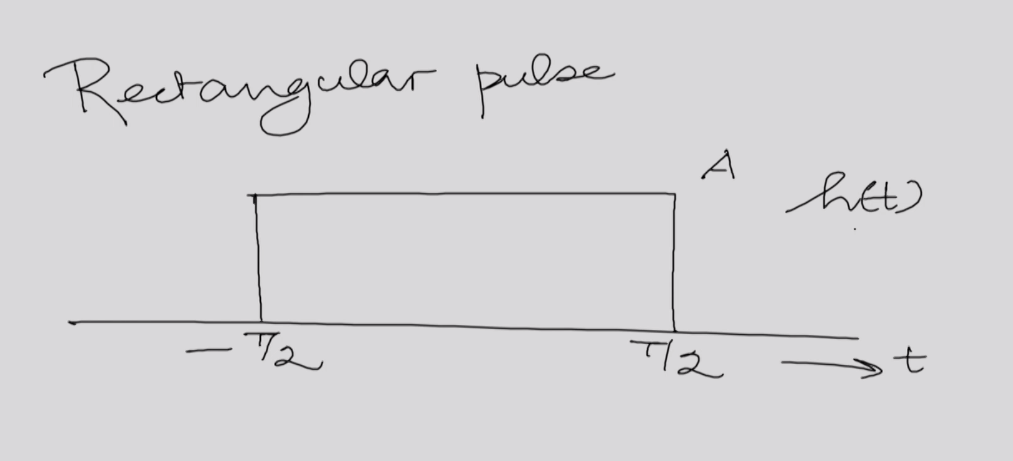
\includegraphics[width=12cm]{rectangularpulse.png}
		\caption{Symmetric Rectangular Pulse}
		\label{fig:rectangular_pulse}
	\end{figure}
	%%%
	Let us denote the Fourier transform by $ H(\Omega)$. Then
	\begin{equation}
		H(\Omega)=\int_{-\infty}^{\infty} \! {h(t) e^{-j\Omega t}} \ \dm t
	\end{equation}
	As $h(t)$ is zero except in the time interval $-T/2$ to $T/2$, we can write the above equation as
	\begin{equation}
		H(\Omega)=\int_{-T/2}^{T/2} \! {A e^{-j\Omega t}} \ \dm t =
		\frac{A e^{-j\Omega t}}{-j \Omega} \Bigg|_{-T/2}^{T/2}=
		\frac{A(e^{-j\Omega T/2}-e^{j\Omega T/2})}{-j\Omega}
		=\frac{AT (2j\sin({\Omega T/2}))}{j\Omega T}
	\end{equation}

	\begin{equation}
		H(\Omega)=\frac{AT\sin({\Omega T/2})}{\Omega T/2}
	\end{equation}
	And we can rewrite it as

	\begin{equation}
		H(f)=\frac{AT \sin({2\pi f T/2})}{2\pi f T/2}
	\end{equation}
	Where $f = \cfrac{\Omega}{2\pi}$ corresponds to the ${cycles}/{second}$ frequency, and $\Omega$ is of course the angular frequency.
	Now this expression also can be written as
	\begin{equation}
		H(\gamma)=\frac{AT \sin({\pi \gamma})}{\pi \gamma}
	\end{equation}
	Where $\gamma = f*T $.\\
	The function $\cfrac{\sin{\pi \gamma}}{\pi \gamma}$ is a very special function called a \emph{Sinc Function}. The sinc function in the form presented is often used in the context of signals and systems.

	\subsubsection{Sketch of the Sinc function}

		Here are the some properties of the Sinc function.
		\begin{itemize}
			\item It is an even function.
			\item It has nulls at every integer; so at 1, at 2, at 3 and so on, it will have value equal to zero.
			\item It tends to 1 as $\gamma$ tends to 0
			\item It is a damped sinusoid, i.e. the magnitude of oscillation decreases as $\gamma$ increases.
		\end{itemize}
		Using the above points we can sketch the Sinc function. So the sketch somewhat looks like Fig\ref{fig:sinc}.
		\begin{figure}[htp]
			\centering
			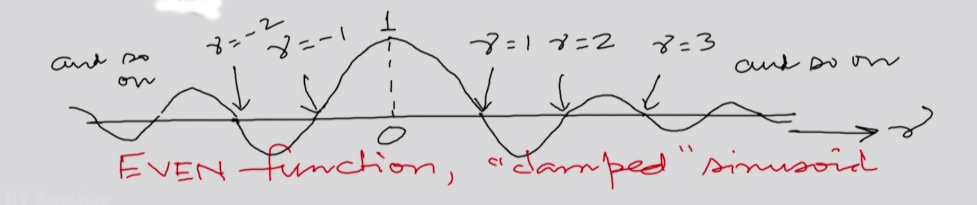
\includegraphics[width=12cm]{sinc.png}
			\caption{Sinc Function}
			\label{fig:sinc}
		\end{figure}

	\subsubsection{Important points regarding the Fourier transform of rectangular pulse}
		The pulse is limited in terms of its occupancy of the time axis. It goes only from  $-T/2$ to $+T/2$. On the other hand, the Fourier transform, in principle, lasts all over the frequency axis.
		What this means is that if we want to make a function vanish all over the time axis outside a certain finite interval, we have to bring together frequencies of all magnitudes and signs except for a few nulls.
		All these frequencies need to come together, in appropriate amplitudes, to form this rectangular pulse. Also note that the Fourier transform for this case is purely real. \\
		 When the pulse width is halved, the nulls of the Fourier transform are doubly spaced and the central amplitude is halved. This can be checked mathematically. We can see that Fig\ref{fig:pulse_FT_half}.
		\begin{figure}[htp]
			\centering
			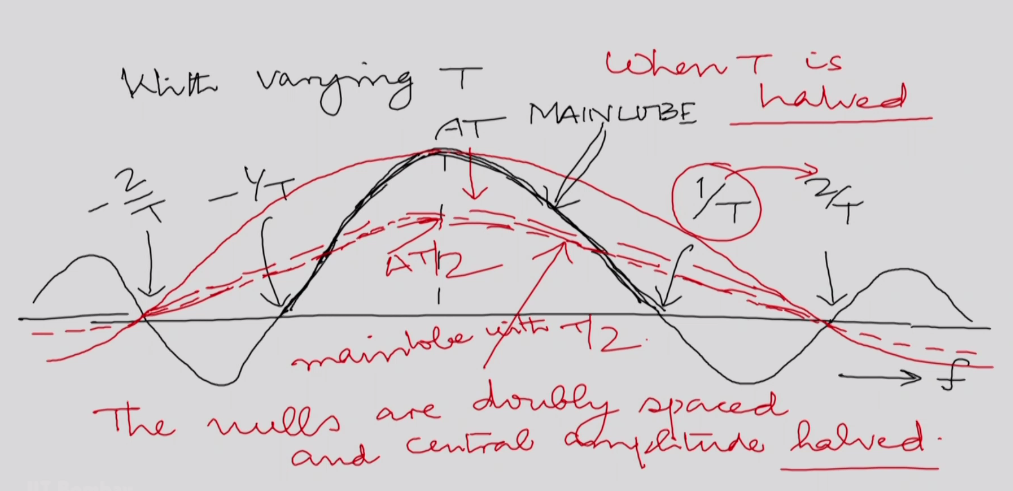
\includegraphics[width=12cm]{pulse_FT_half.png}
			\caption{Fourier Transform of Rectangular Pulse at width T and T/2 }
			\label{fig:pulse_FT_half}
		\end{figure}

\subsection{Properties of Fourier Transform}
	Let us see what happens to the Fourier transform when we change the original signal in some particular way.
	% When we change the signal in some way or when we bring signals together, what happens to the corresponding Fourier transform is what we will investigate in this section.
	\subsubsection{Linearity}
		Let $h_1(t)$ have the Fourier transform $H_1(\Omega)$ and let $h_2(t)$ have the Fourier transform $H_2(\Omega)$. Then, linearity says

		%\begin{equation}
		%$$\alpha h_1(t) + \beta h_2(t) \longrightarrow \alpha H_1(\Omega)+ \beta H_2(\Omega)$$
		%\end{equation}


		\[\alpha h_1(t) + \beta h_2(t) \xrightarrow{\mathcal{F}} \alpha H_1(\Omega)+ \beta H_2(\Omega)\]
		for all $\alpha$, $\beta$ $\in \mathbb{C}$ and all $h_1(t)$ and $h_2(t)$. Here, ${\mathcal{F}}$ means ``has the Fourier transform given by".

	\subsubsection{Proof of linearity}
		\begin{equation}
			 \alpha \{ H_1(\Omega) \} = \alpha \{ \int_{-\infty}^{\infty} \! h_1(t)e^{-j\Omega t} \ \dm t \}
			\label{eqn:one}
		\end{equation}

		\begin{equation}
			 \beta \{ H_2(\Omega) \} = \beta \{ \int_{-\infty}^{\infty} \! h_2(t)e^{-j\Omega t} \ \dm t \}
			\label{eqn:two}
		\end{equation}
		Add Eqn.\ref{eqn:one} and \ref{eqn:two}. We can write it as
		\begin{equation}
			\{ \alpha H_1(\Omega) + \beta H_2(\Omega) \} = \{ \int_{-\infty}^{\infty} \! (\alpha h_1(t) + \beta h_2(t))e^{-j\Omega t} \ \dm t \}
		\end{equation}

	\subsubsection{The Inverse Fourier transform}
		THe Inverse Fourier transform can be written as
		\begin{equation}
			H_1(\Omega) \xrightarrow{\mathcal{F}^{-1}} \frac{1}{2\pi} \int_{-\infty}^{\infty} \! H_1(t) e^{j\Omega t} \ \dm \Omega
		\end{equation}
		Note that $\Omega$ = $2\pi f$ and $d\Omega$= $2\pi df$. Hence,
		%%%
		\begin{equation}
			H_1(f) \xrightarrow{\mathcal{F^-1}} \int_{-\infty}^{\infty} \! H_1(f) e^{j2\pi ft} \ \dm f
		\end{equation}
		%%%
		Where $\Omega$ =  Radians/sec frequency
		And $f$ = cycles/sec frequency
		%%%
		\begin{itemize}
			\item We can clearly see that when frequency is in radians/sec then, we will have factor of $1/2\pi$ in the inverse Fourier transform and when frequency is in cycles/sec then the factor of $1/2\pi$ will not be there.
			\item In a way dealing with cycles/second frequency has some conveniences; we don't need to remember the factor of $1/2\pi$, or we can say, there is a perfect symmetry between the Fourier transform and the Inverse Fourier transform.
		\end{itemize}

	\subsubsection{Exercise}
		 Prove that linearity holds true for the inverse Fourier transform.

\subsection{Time Shift}
	What happens to the Fourier transform when we shift the signal in time? If
	\begin{equation}
		h(t) \xrightarrow{\mathcal{F}} H(\Omega)
	\end{equation}
	then, for a constant $\tau$,
	\begin{equation}
		h(t-\tau) \xrightarrow{\mathcal{F}} {?}
	\end{equation}
	%%%
	The Fourier transform would be
	\begin{equation}
		H(\Omega) =  \int_{-\infty}^{\infty} \! h(t-\tau) e^{-j\Omega t} \ \dm t
	\end{equation}
	Put $(t-\tau) = \lambda$  $\Rightarrow$  $t = \tau + \lambda$.
	So the Fourier transform is
	\begin{equation}
		H(\Omega) =  \int_{-\infty}^{\infty} \! h(\lambda) e^{-j\Omega (\lambda + \tau)} \ \dm \lambda =
		e^{-j\Omega \tau} \int_{-\infty}^{\infty} \! h(\lambda) e^{-j\Omega \lambda} \ \dm \lambda
	\end{equation}
	So,
	\begin{equation}
		h(t-\tau) \xrightarrow{\mathcal{F}} e^{-j\Omega \tau} H(\Omega)\   or\   e^{-j2\pi f\tau} H(f)
	\end{equation}
	Now it can be clearly seen that
	\begin{itemize}
		\item The magnitude of the Fourier transform is unchanged.
		\item The angle or the phase of the Fourier transform changes.
	\end{itemize}

	\subsubsection{Modulation}
		By modulation, we mean multiplying $h(t)$ by a rotating complex number (rotating with an angular velocity of $\Omega_0$). In this case, the Fourier transform is shifted by $\Omega_0$ forward.

		\begin{equation}
			e^{j\Omega_0 t} h(t) \xrightarrow{\mathcal{F}} {?}
		\end{equation}
		So the Fourier transform would be
		\begin{equation}
			 \int_{-\infty}^{\infty} \! e^{j\Omega_0 t} h(t) e^{-j\Omega t} \ \dm t =
			 \int_{-\infty}^{\infty} \! h(t) e^{-j(\Omega-\Omega_0) t} \ \dm t =
			 H(\Omega-\Omega_0)
		\end{equation}
		
		\begin{itemize}
			\item When we shift a function in time, it causes a modulation in the frequency domain (We remember, it multiplied the Fourier transform by a term $e^{-j\Omega \tau_0}$).

			\item When we modulate the function in time by multiplying by a rotating complex number, the corresponding Fourier transform shifts in frequency.

			\item Basically, shift in time becomes modulation in frequency, and modulation in time becomes a shift in frequency.
		\end{itemize}

	\subsubsection{Convolution Property of Fourier transform}
		The question to answer here is what will be the Fourier transform of $x_1(t)*x_2(t)$, given that the Fourier transforms of $x_1(t)$ and $x_2(t)$ are $X_1(\Omega)$ and $X_2(\Omega)$ respectively. 

		\begin{equation}
			x_1(t)\ast x_2(t) = \int_{-\infty}^{\infty}{x_1(\tau) x_2(t-\tau)}d\tau
		\end{equation}

		\begin{equation}
			x_1(t)\ast x_2(t) \xrightarrow{\mathcal{F}} {?}
		\end{equation}
		\noindent
		Now let's solve it. The Fourier transform can be written as
		\begin{equation}
			\int_{-\infty}^{\infty} \! \{ \int_{-\infty}^{\infty} \! x_1(\tau) x_2(t-\tau) \ \dm \tau \} e^{-j\Omega t} \ \dm t
		\end{equation}
		This is same as
		\begin{equation}
			\int_{-\infty}^{\infty} \! \int_{-\infty}^{\infty} \! x_1(\tau) x_2(t-\tau) e^{-j\Omega t} \ \dm \tau \dm t
		\end{equation}
		To solve the above double integral we will do a change of variables. Put
		\begin{equation}
			\alpha =\tau \ \text{and} \ \beta = (t-\tau)
		\end{equation}

		\begin{equation}
			\left( \begin{array}{c}
			\alpha \\
			\beta \end{array} \right)
			=
			\left( \begin{array}{cc}
			1 & 0 \\
			-1 & 1 \end{array} \right)
			\left( \begin{array}{c}
			\tau \\
			 t \end{array} \right)
		\end{equation}

		\begin{equation}
			\mathrm{d}\tau \mathrm{d}t = |\text{Det(transformation)}| \mathrm{d}\alpha \mathrm{d}\beta
		\end{equation}
		\noindent
		Hence,
		\begin{equation}
			\mathrm{d}\tau \mathrm{d}t = \mathrm{d}\alpha \mathrm{d}\beta
		\end{equation}
		Hence, the element of integration also remains the same because the Jacobian is $1$. Now the modified integral is
		
		\begin{equation}
			\int_{-\infty}^{\infty} \! \int_{-\infty}^{\infty} \! x_1(\alpha) x_2(\beta) \exp{-j\Omega(\alpha+\beta)} \ \dm \alpha \dm \beta
		\end{equation}
		
		\begin{equation}
			=\int_{-\infty}^{\infty} \! x_1(\alpha) \{ \int_{-\infty}^{\infty} \!
			x_2(\beta) e^{-j\Omega(\beta)} \ \dm \beta \} e^{-j\Omega \alpha} \ \dm \alpha
		\end{equation}
		This can be written as
		
		\begin{equation}
			X_2(\Omega) \int_{-\infty}^{\infty} \! x_1(\alpha) e^{-j\Omega \alpha} \ \dm \alpha
		\end{equation}
		So
		\begin{equation}
			x_1(t) \ast x_2(t) \xrightarrow{\mathcal{F}} X_1(\Omega)X_2(\Omega)
		\end{equation}
		\noindent
		Hence a convolution in the natural domain becomes a multiplication in the Fourier domain.

\subsection {Conclusion} In this section, we discussed about the Fourier transform of a rectangular pulse which is the ``Sinc function'', and its properties. We showed some of the properties of Fourier transform and their proofs.
\section{Module 2: Lecture 8\\Convolution Property of the Fourier Transform}

\subsection{Introduction}
	In this section, we will talk about the properties of the Fourier transform and specifically, we see more about the convolution property.
\subsection{Convolution Theorem}
	If two signals $x_1(t)$ and $x_2(t)$ both have Fourier transforms, which are $X_1(\Omega)$ and $X_2(\Omega)$ respectively, and if their convolution also has a Fourier transform, then this Fourier Transform is equal to the product of $X_1(\Omega)$ and $ X_2(\Omega)$.\\
	Mathematically,
	\begin{align}
		x_1(t) \xrightarrow{\mathcal{F}}& X_1(\Omega)\\
		x_2(t)\xrightarrow{\mathcal{F}}& X_2(\Omega)\\
		x_1(t)*x_2(t)\xrightarrow{\mathcal{F}}& X_1(\Omega).X_2(\Omega)
	\end{align}
	So, when we apply it to the context of LSI systems, we get
	\begin{equation}
		Y(\Omega)=X(\Omega)H(\Omega)
	\end{equation}
	where,
	\begin{align}
		x(t) &\xrightarrow{\mathcal{F}} X(\Omega)\\
		y(t) &\xrightarrow{\mathcal{F}} Y(\Omega)\\
		h(t) &\xrightarrow{\mathcal{F}} H(\Omega)
	\end{align}
	\begin{figure}[ht]
		\centering
		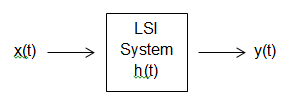
\includegraphics{fig0.png}
		%\caption{\label VVoltage generator (side view)}
	\end{figure}
	We said that there is a point-wise decoupling or memorylessness in the Fourier domain, meaning, the output at angular frequency $\Omega$ depends only on the input at angular frequency $\Omega$ and the impulse response at angular frequency $\Omega$ and none other.\\
	Where does this come from?\\
	$X(\Omega)$ is the component of input at angular frequency $\Omega$. Let us imagine $X(\Omega)e^{j\Omega t}$ as an input to the LSI system, where $X(\Omega)$ is a complex number.\\
	We have,
	\begin{figure}[h!]
		\centering
		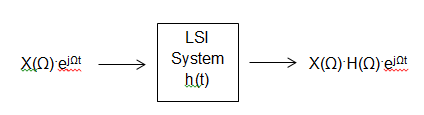
\includegraphics{fig1.png}
		%\caption{\label VVoltage generator (side view)}
	\end{figure}
	\begin{align}
		y(t) &= \int_{-\infty}^{\infty} \! h(\tau) X(\Omega) \ e^{j\Omega (t-\tau)} \ \dm \tau\\
		&= \left( \int_{-\infty}^{\infty} \! h(\tau) \ e^{-j\Omega \tau} \ \dm \tau \right) X(\Omega) \ e^{j\Omega t}\\
		&= X(\Omega) H(\Omega) \ e^{j\Omega t}
	\end{align}
	$H(\Omega)$ is the component of the impulse response along $e^{j\Omega t}$. Hence, $X(\Omega).H(\Omega)$ is the component of $y(t)$ along $e^{j\Omega t}$ and is equal to $Y(\Omega)$.\\
	\begin{equation}
		Y(\Omega)=X(\Omega).H(\Omega)
	\end{equation}
	%%%
	%%% CHECK THE FOLLOWING PART:
	This is analogous to an operator acting upon a force in mechanics. If $\nabla$ is the operator and if $\vec{F}$ the force vector such that
	\begin{equation}
	\vec{F}=F_x \hat{x} + F_y \hat{y} + F_z \hat{z}
	\end{equation}
	Then
	\begin{eqnarray}
	\nabla . \vec{F} &=& \nabla . (F_x \hat{x} + F_y \hat{y} + F_z \hat{z})\\
	\nabla . \vec{F} &=& \partial_x F_x \hat{x} + \partial_y F_y \hat{y} + \partial_z F_z \hat{z}\\
	\end{eqnarray}
	Similarly we resolve the input into its components along the different $\Omega$'s, i.e. $ej\Omega  t$.
	\begin{eqnarray}
	x(t)&=&\sum_i X(\Omega_i).\textrm{exp}(j\Omega_i t)\\
	y(t)&=&\sum _i X(\Omega_i).H(\Omega_i).\textrm{exp}(j\Omega_i t)
	\end{eqnarray}
	In a way, the idea is to decouple the action of the LSI system when we think of the input as comprising of different complex exponentials rotating at different angular frequencies, both positive and negative.
	%%%
	%%%
\subsection{What is a transform?}
	More generally, transform is a change of paradigm. Paradigm means world view. In a system point of view, a signal is a mapping from the independent variable to complex numbers, while a system is a mapping from signals to signals. Whereas a transform is a mapping of the signals and systems altogether to the transformed domain of signals and systems.
\subsection{Convolution or Multiplication}
	Doing multiplication, in general, is easier than convolution. To find the convolution, take Fourier transforms of the two signals, multiply them and then take its inverse Fourier transform.
	\begin{align}
		x_1(t) &\xrightarrow{\mathcal{F}} X_1(\Omega)\\
		x_2(t) &\xrightarrow{\mathcal{F}} X_2(\Omega)\\
		X_1(\Omega).X_2(\Omega) &\xrightarrow{\mathcal{F}^{-1}} x_1(t) \ast x_2(t)
	\end{align}
	It is beneficial only if the Fourier transform operations are easier to perform, otherwise it is not always better to go through the Fourier domain.\\
	For example, take $x_1(t)=x_2(t)$ as a rectangular pulse as shown in Fig\ref{fig:rectangular_pulse}.
	\begin{figure}[h!]\label{fig:rectangular_pulse}
		\centering
		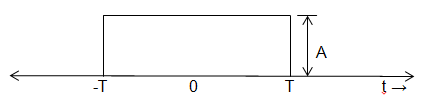
\includegraphics{fig2.png}
	\end{figure}
	Hence,
	\begin{align}
		X_1(\Omega)=X_2(\Omega) &= \int_{-\infty}^{\infty} \! x_1(t) \ e^{-j\Omega t} \ \dm t\\
		&= \int_{-T}^{T} \! A \ e^{-j\Omega t} \ \dm t\\
		&= \left(\frac{A}{-j\Omega} \ e^{-j\Omega t}\right) \Bigg|_{-T}^{T}\\
		&= \frac{2Aj \sin(\Omega t)}{j\Omega} \times \frac{T}{T}\\
		&= 2AT \frac{\sin{\Omega T}}{\Omega T}
	\end{align}
	Whereas the convolution leads to
	\begin{equation}
		x_1(t) \ast x_2(t)=\int_{-\infty}^{\infty} \! x_1(\tau)x_2(t-\tau) \ \dm \tau
	\end{equation}
	Now, $x_1(\tau) x_2(t-\tau)$ is non-zero only when some area of both the pulses coincide and is non- zero for that range only.
	This happens only for $t \in [-2T,2T]$
	\begin{figure}[h!]
	\centering
	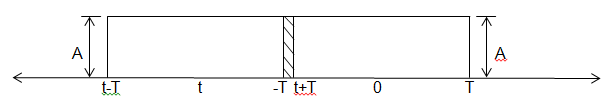
\includegraphics[scale=0.9]{fig3.png}
	\end{figure}
	Therefore, for $t \in [-2T,0]$
	\begin{align}
		x_1(t) \ast x_2(t) &= \int_{-\infty}^{\infty} \! x_1(\tau)x_2(t-\tau) \ \dm \tau\\
		&= \int_{-T}^{t+T} \! A^2 \ \dm \tau \\
		&= A^2 (t+2T)
	\end{align}
	and for $t \in [0,2T]$
	\begin{align}
		x_1(t) \ast x_2(t) &= \int_{-\infty}^{\infty} \! x_1(\tau)x_2(t-\tau) \ \dm \tau\\
		&= \int_{t-T}^{T} \! A^2 \ \dm \tau \\
		&= A^2 (2T-t)
	\end{align}
	\begin{figure}[ht]
		\centering
		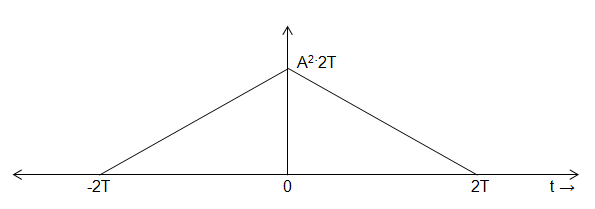
\includegraphics[scale=0.9]{fig4.png}
	\end{figure}
	Now the Fourier transform of $x_1(t)*x_2(t)$ is $X_1(\Omega)X_2(\Omega)$ which is equal to	
	\begin{equation}
		X_1(\Omega)X_2(\Omega) = \left( 2AT \frac{\sin(\Omega T)}{\Omega T} \right) ^2
	\end{equation}

\subsection{The Principle of Duality}

	We know that
	\begin{equation}
		X(\Omega) = \int_{-\infty}^{\infty} \! x(t) e^{-j\Omega t} \ \mathrm{d}t
	\end{equation}	
	and
	\begin{equation}
		x(t) = \frac{1}{2\pi}\int_{-\infty}^{\infty} \! X(\Omega) e^{j\Omega t} \ \mathrm{d}\Omega
	\end{equation}
	Now, in the second integral, let's interchange `$t$' and `$\Omega$'. Hence,
	\begin{equation}
		x(\Omega) = \frac{1}{2\pi}\int_{-\infty}^{\infty} \! X(t) e^{j\Omega t} \ \mathrm{d}t
	\end{equation}
	Hence,
	\begin{equation}
		x(-\Omega) = \frac{1}{2\pi}\int_{-\infty}^{\infty} \! X(t) e^{-j\Omega t} \ \mathrm{d}t
	\end{equation}
	Hence,
	\begin{equation}
		2\pi [x(-\Omega)] = \int_{-\infty}^{\infty} \! X(t) e^{-j\Omega t} \ \mathrm{d}t
	\end{equation}
	This shows that, if
	\begin{equation}
		x(t) \xrightarrow{\mathcal{F}} X(\Omega)
	\end{equation}
	then
	\begin{equation}\label{eqn:duality}
	X(t) \xrightarrow{\mathcal{F}} 2\pi [x(-\Omega)]
	\end{equation}
	This is the principle of duality for the Fourier transform. \\
	Let us take the example of the same rectangular pulse which we considered in the earlier section. The Fourier transform of the rectangular pulse is given by
	\begin{equation}
		X(\Omega) = 2AT \frac{\sin(\Omega T)}{\Omega T}
	\end{equation}
	Let us invoke duality here. We will replace $T$ by $W$ for convenience of notation Hence,
	\begin{equation}
		X(t) = 2AW \frac{\sin{(W t)}}{W t} \xrightarrow{\mathcal{F}} 2\pi [x(-\Omega)]
	\end{equation}
	Here, $2\pi x(\Omega)$ is the rectangular pulse with width $2W$ and height $2\pi A$. As the pulse is symmetric, $x(-\Omega) = x(\Omega)$.\\
	We can see why this is a very useful property. Say you want to evaluate the convolution of $\sin(Wt)/Wt$. It is very difficult to evaluate it using the direct expression of the convolution. But, we can invoke the principle of duality here. We know that the Fourier transform of a convolution is the product of their Fourier transforms. Hence, applying this to $X(t)$,
	\[
	X(t)*X(t) \xrightarrow{\mathcal{F}} [2\pi x(\Omega)]^2
	\]
	Now, it is very easy to evaluate the right hand side. It is in fact the same symmetric rectangular pulse, but with height $(2\pi A)^2$. Hence, it is equal to $(2\pi)^2 A x(\Omega)$. Therefore, we have,
	\begin{equation}\label{eqn:sinc_convolution}
	X(t)*X(t) \xrightarrow{\mathcal{F}} (2\pi)^2 A \ x(\Omega)
	\end{equation}
	Now, we know from the principle of duality (Eqn.\ref{eqn:duality}), that
	\begin{equation}
		X(t) \xrightarrow{\mathcal{F}} 2\pi [x(-\Omega)]
	\end{equation}
	Comparing this with Eqn.\ref{eqn:sinc_convolution}, we get,
	\begin{equation}
		X(t)*X(t) = 2\pi A \ X(t) = 2\pi A \left( 2AW \frac{\sin(Wt)}{Wt} \right)
	\end{equation}
	Hence, the evaluation of the convolution of $\sin(Wt)/Wt$ and other complicated functions with themselves can become a lot easier and straightforward if we invoke the principle of duality.

\section{Module 2: Lecture 9\\Multiplication Theorem and Parseval's Theorem}


\subsection{Introduction}
We have seen in the last few sessions, the property of duality and the convolution – multiplication parallel. We will now see the implications of duality, deriving what we call ‘Multiplication theorem’ and then its application called the ‘Parseval’s theorem’.

\subsection{Multiplication}
Let us take $x_1(t)$ and $x_2(t)$ with Fourier transforms $X_1(\Omega)$ and $X_2(\Omega)$ respectively. We derived earlier the Fourier transform of $x_1(t) \ast x_2(t)$ to be $X_1(\Omega)X_2(\Omega)$. We shall now try to find a general expression for the Fourier transform of the product $x_1(t)x_2(t)$.
\\
We have,            
\begin{equation}
x_1(t)\xrightarrow{\mathcal{F}} X_1(\Omega)
\end{equation}
\begin{equation}
x_2(t) \xrightarrow{\mathcal{F}} X_2(\Omega)
\end{equation}
\begin{equation}
x_1(t) \ast x_2(t)\xrightarrow{\mathcal{F}} X_1(\Omega)X_2(\Omega)
\end{equation}

Applying duality on (3) gives
\[
X_1(t)X_2(t)
\xrightarrow{\mathcal{F}}
2\pi (x1 \ast x2)(-\Omega)
\]
Also by duality,

\[
X_1(t)
\xrightarrow{\mathcal{F}}
2 \pi x_1(-\Omega)
\]
\[
X_2(t)
\xrightarrow{\mathcal{F}}
2 \pi x_2(-\Omega)
\]

$2\pi x_1(-\Omega) \ast x_2(-\Omega)$, which is the Fourier transform of $X_1(t)X_2(t)$, can be re-written as,
\[
\frac{1}{2\pi} ( 2\pi x_1(-\Omega) * 2\pi x_2(-\Omega) )
\]
Notice that $2\pi x_1(-\Omega)$ is the Fourier transform of $X_1(t)$ and $2\pi x_2(-\Omega)$ is the Fourier transform of $X_2(t)$.
Therefore we can see that the Fourier transform of the product $X_1(t)X_2(t)$ is the convolution of Fourier transforms of the individual time domain functions multiplied by a factor of $\frac{1}{2\pi}$. 

\subsubsection*{Theorem}
If 
\[
y_1(t)
\xrightarrow{\mathcal{F}} Y_1(\Omega)
\]
\[
y_2(t)
\xrightarrow{\mathcal{F}}
Y_2(\Omega)
\]
Then the Fourier transform the product (provided all the Fourier transforms exist) is,
\begin{equation}
y_1(t)y_2(t) 
\xrightarrow{\mathcal{F}}
\frac{1}{2\pi} 
( Y_1(\Omega) \ast Y_2(\Omega) )
\end{equation}
Multiplication of one signal by another can be thought of as using one signal to scale or modulate the amplitude of the other, and consequently, the multiplication of two signals is often referred to as 'amplitude modulation'. For this reason, (4) is sometimes referred to as the modulation property.


\subsubsection*{Special Case of Multiplication Theorem}
We have seen from the multiplication theorem, if $y_1(t)$ and $y_2(t)$ have the following Fourier transforms, 

\[
y_1(t)
\xrightarrow{\mathcal{F}}
Y_1(\Omega)
\]\[
y_2(t)
\xrightarrow{\mathcal{F}}
Y_2(\Omega)
\]
then
\[
y_1(t) y_2(t) 
\xrightarrow{\mathcal{F}}
\frac{1}{2\pi}
{ Y_1(\Omega) \ast Y_2(\Omega) }
\]
Let us find the Fourier transform of $y_1(t)\overline{y_2(t)}$:
We will first find out the Fourier transform of $\overline{y_2(t)}$ and then get the Fourier transform of $y_1(t)$ in two different ways:\begin{enumerate}
\item Using the multiplication theorem.
\item By the general definition of Fourier transform of any given function.
\end{enumerate}
First, the Fourier transform of  $\overline{y_2(t)}$:
The inverse Fourier transform of a given function $X(\Omega)$ is given by 
\[
x(t) = \frac{1}{2\pi}\int_{-\infty}^{\infty}{ X(\Omega) 
e^{j \Omega t}d\Omega }
\]
Taking the complex conjugate of the above,
\[	
\overline{x(t)} = \frac{1}{2\pi}\int_{-\infty}^{\infty}{\overline{X(\Omega)}e^{-j \Omega t}d\Omega }
\]  
Transforming $\Omega$ with $-\alpha$,
\begin{equation}
\overline{x(t)} = \frac{1}{2\pi}\int_{-\infty}^{\infty}{\overline{X(-\alpha)}e^{j \alpha t}d\alpha }
\end{equation}
From equation (5) we can observe that the Fourier transform of  $\overline{x(t)}$ is $\overline{X(-\alpha)}$.
Therefore 
\[
\overline{y_2(t)}
\xrightarrow{\mathcal{F}}
\overline{Y_2(-\Omega)}
\]
\noindent
From multiplication theorem, we can get the Fourier transform of the product $y_1(t)\overline{y_2(t)}$
\[
y_1(t)\overline{y_2(t)}
\xrightarrow{\mathcal{F}}
\frac{1}{2\pi} { 
Y_1(\Omega) 
\ast 
\overline{Y_2(-\Omega)}}\]
We can also obtain the Fourier transform using the general definition, i.e
\[
y_1(t)\overline{y_2(t)} \xrightarrow{\mathcal{F}}
\int_{-\infty}^{\infty}
{ y_1(t)\overline{y_2(t)} e^{-j\Omega t}dt }
\]

The Fourier transforms of $y_1(t)\overline{y_2(t)}$  obtained by either method should be identical, and hence we can write,
\[
\frac{1}{2\pi} { Y_1(\Omega)
 \ast \overline{Y_2(-\Omega)}} = 
\int_{-\infty}^{\infty}
{ y_1(t)\overline{y_2(t)} e^{-j\Omega t}dt }
\]

\[
\frac{1}{2\pi}
\int_{-\infty}^{\infty} \!
{Y_1(\Omega - \lambda)\overline{Y_2(-\lambda)}\ \mathrm{d}\lambda}
= 
\int_{-\infty}^{\infty}
{ y_1(t)\overline{y_2(t)} e^{-j\Omega t}dt }
\]

In the above equation, put $\Omega  =0$, the identity becomes
\[
\frac{1}{2\pi}
\int_{-\infty}^{\infty}
{Y_1(-\lambda)\overline{Y_2(-\lambda)}d\lambda}
= 
\int_{-\infty}^{\infty}
{ y_1(t)\overline{y_2(t)}dt }
\]

In the left hand side integral above, transform using $-\lambda \rightarrow \beta$, then
$d\lambda \rightarrow -d\beta$, and as $\lambda$ goes from $-\infty$ to $+\infty$, $\beta$ goes from $+\infty$ to $-\infty$. 
The equation becomes
\[
\frac{1}{2\pi} 
\int_{-\infty}^{\infty}
{ Y_1(\beta) 
\overline{Y_2(\beta)} d\beta } = \int_{-\infty}^{\infty}
{ y_1(t) \overline{y_2(t)}  dt } 
\]

Observe that the right hand side is essentially the inner product of $y_1(t)$ and $y_2(t)$  and the left hand side is the inner product of $Y_1(\Omega)$ and   $Y_2(\Omega)$ multiplied by a factor of $\frac{1}{2\pi}$.  Essentially, arrived at an equivalence between inner products in time domain and inner product in frequency domain. This is called the Parseval's theorem. 

\subsubsection*{Theorem}
If $y_1(t)$ and $y_2(t)$ have respectively their Fourier transforms $Y_1(\Omega)$ and $Y_2(\Omega)$, then the inner product of $y_1(t)$ and $y_2(t)$ is $\frac{1}{2\pi}$ times the inner product of $Y_1(\Omega)$ and $Y_2(\Omega)$
\[
\int_{-\infty}^{\infty}
{ y_1(t) \overline{y_2(t)} dt }  = \frac{1}{2\pi} 
\int_{-\infty}^{\infty}
{ Y_1(\Omega) \overline{Y_2(\Omega)} d\Omega }
\]









                



                     

\section{Module 2: Lecture 10\\Spectral Density}

\subsection{Introduction}
\noindent
In the previous lecture, we derived the multiplication property of the Fourier Transform which subsequently led to the derivation of Parseval’s Theorem. 
In this lecture, we will see more on the interpretation of the Parseval’s theorem as the invariance of the inner product of two signals calculated in time and angular frequency (or Fourier) domain. 
We will also define the energy of a signal and relate it with the Parseval’s Theorem and introduce the notion of Spectral Density of a signal.
Having done that, we will introduce the differentiation property of the Fourier Transform and its dual which will help us in calculating Fourier transforms of many more signals from the already known simpler Fourier transforms.
\subsection{Invariance of Inner Product on Change of Basis}
The property
\[
\int\limits_{-\infty}^{\infty}x(t)\overline{y(t)} dt = \cfrac{1}{2\pi}\int\limits_{-\infty}^{\infty}X(\Omega)\overline{Y(\Omega)} d\Omega
\]
has a deeper implication when we think of this in terms of the inner product of $x$ and $y$. Recall from vector algebra that in two dimensions, we can write any vector $\overrightarrow{v}$ as a linear combination of any two orthonormal basis vectors. Consider two such vectors, and two different sets of orthonormal vectors, such that
\[
\overrightarrow{v_1}=v_{11}\hat{u}_1+v_{12}\hat{u}_2 = v_{13}\hat{u}_3+v_{14}\hat{u}_4
\]
and
\[
\overrightarrow{v_2}=v_{21}\hat{u}_1+v_{22}\hat{u}_2 = v_{23}\hat{u}_1+v_{24}\hat{u}_4
\]
Now, the inner product or the dot product between the two vectors is the magnitude of one vector times the projection of the second vector along the first vector. The important thing to note here is that the inner product is a property of the vectors in themselves. This inner product, by definition, \emph{does not depend on which basis we choose to express them}. Thus,
\[
\overrightarrow{v_1}.\overrightarrow{v_2}=v_{11}v_{21}+v_{12}v_{22} = v_{13}v_{23}+v_{14}v_{24}
\]

This is exactly what the meaning of Parseval's theorem is. In the time domain, the basis vectors used, as you can remember from the first model, are the unit impulses:
\[
x(t) = \int_{-\infty}^{+\infty} \! x(\lambda)\delta(t-\lambda) \ \mathrm{d}\lambda
\]
Whereas in the frequency domain, the basis vectors are the rotating complex numbers or phasors:
\[
X(\Omega) = \int_{-\infty}^{+\infty} \! x(\lambda)e^{-j\Omega\lambda} \ \mathrm{d}\lambda
\]
But the inner product between two signals remains independent of the basis, which is what the Parseval's theorem states.
\[
\int\limits_{-\infty}^{\infty}x(t)\overline{y(t)}dt = \cfrac{1}{2\pi}\int\limits_{-\infty}^{\infty}X(\Omega)\overline{Y(\Omega)}d\Omega
\]
The factor of $2\pi$ arises due to the same reason why it arrived in the inverse Fourier transform, which is the normalization of the complex exponential.
\subsection{Energy of a Signal}
\noindent
The energy $E_x$ of a continuous time signal $x(t)$ is defined as

$$E_x = \int\limits_{-\infty}^{\infty}|x(t)|^2dt$$

\subsubsection{Relating Energy of a Signal and Parseval's Theorem}
\noindent
Consider two continuous time signals $x(t)$ and $y(t)$ with Fourier Transforms $X(\Omega)$ and $Y(\Omega)$ respectively. Then Parseval's theorem states that,

$$\int\limits_{-\infty}^{\infty}x(t)\overline{y(t)}dt = \cfrac{1}{2\pi}\int\limits_{-\infty}^{\infty}X(\Omega)\overline{Y(\Omega)}d\Omega$$

\noindent
where $(\cdot)^*$ denotes the complex conjugate of the corresponding signal.

\noindent
Now, if we substitute $y(t) = x(t)$ in the above relation, we get,

$$\int\limits_{-\infty}^{\infty}x(t)\overline{x(t)}dt = \cfrac{1}{2\pi}\int\limits_{-\infty}^{\infty}X(\Omega)\overline{X(\Omega)}d\Omega$$

\noindent
Since, $x(t)\overline{x(t)} = |x(t)|^2$ and $X(\Omega)\overline{X(\Omega)} = |X(\Omega)|^2$ we get,

$$\int\limits_{-\infty}^{\infty}|x(t)|^2dt = \cfrac{1}{2\pi}\int\limits_{-\infty}^{\infty}|X(\Omega)|^2d\Omega$$

\noindent
From the above relation, we see that the energy of a signal can also be calculate using the formula,

$$E_x = \cfrac{1}{2\pi}\int\limits_{-\infty}^{\infty}|X(\Omega)|^2d\Omega$$

\subsubsection{Energy Spectral Density}
\noindent
We have seen that if a signal $x(t)$ has a Fourier Transform $X(\Omega)$, its energy can be calculated from the angular frequency domain using the formula,

$$E_x = \cfrac{1}{2\pi}\int\limits_{-\infty}^{\infty}|X(\Omega)|^2d\Omega$$

\noindent
Integrating $|X(\Omega)|^2$ over the entire angular frequency axis and multiplying the result by $\cfrac{1}{2\pi}$ gives us the energy of the signal.

\noindent
Thus $|X(\Omega)|^2$ conveys the distribution of energy along the angular frequency axis.

\noindent
Hence, the integrand $|X(\Omega)|^2$ in the above formula is of significance and is called the Energy Spectral Density of the signal $x(t)$.

\subsubsection{Energy Spectral Density and Linear Shift-Invariant Systems}
\noindent
Consider a linear shift invariant system having an impulse response $h(t)$ and let $y(t)$ be the output  of this system when an input $x(t)$ is applied to it.

\noindent
Then, we have

$$y(t) = x(t)*h(t)$$

\noindent
where $*$ denotes the convolution operator.

\noindent
Assume that the Fourier transforms of $h(t)$ and $x(t)$. Let $H(\Omega)$ and $X(\Omega)$ be their respective Fourier Transforms.

\noindent
Then the Fourier Transform $Y(\Omega)$ of the signal $y(t)$ is given by.

$$Y(\Omega) = X(\Omega)H(\Omega)$$

\noindent
Therefore,

$$|Y(\Omega)|^2 = |X(\Omega)|^2|H(\Omega)|^2$$

\noindent
Note that $|Y(\Omega)|^2$, $|X(\Omega)|^2$ and $|H(\Omega)|^2$ are essentially the energy spectral densities of the signals $y(t)$, $x(t)$ and the impulse response $h(t)$ respectively.

\noindent
Thus, the energy spectral density of the output is equal to the energy density of the input multiplied by the energy density of the frequency response.

\subsection{The Differentiation Property of the Fourier Transform}


\noindent
Consider a continuous time signal $x(t)$ which has a Fourier transform $X(\Omega)$ then we can write,

$$x(t) = \cfrac{1}{2\pi}\int\limits_{-\infty}^{\infty}X(\Omega)e^{j\Omega t}d\Omega$$

\noindent
Differentiating on both sides with respect to $'t'$ we get,

$$\cfrac{dx(t)}{dt} = \cfrac{d}{dt}\left(\cfrac{1}{2\pi}\int\limits_{-\infty}^{\infty}X(\Omega)e^{j\Omega t}d\Omega\right)$$

\noindent
Taking the derivative under the integral we get,

$$\cfrac{dx(t)}{dt} = \cfrac{1}{2\pi}\int\limits_{-\infty}^{\infty}X(\Omega)\cfrac{de^{j\Omega t}}{dt}d\Omega$$

\noindent
Therefore,

$$\cfrac{dx(t)}{dt} = \cfrac{1}{2\pi}\int\limits_{-\infty}^{\infty}(X(\Omega)j\Omega)e^{j\Omega t}d\Omega$$

\noindent
Comparing the above equation with the definition of the inverse Fourier Transform, we see that for the signal $x(t)$ has the Fourier Transform $j\Omega X(\Omega)$.

\noindent
Thus, the differentiation property of the Fourier transform states that if a continuous variable signal $x(t)$ has the Fourier Transform $X(\Omega)$, then the Fourier transform of $\cfrac{dx(t)}{dt}$ is $j\Omega X(\Omega)$.

\subsubsection{Interpretation of the differentiation property}
\noindent
The differentiation property of the Fourier Transform can be interpreted in the following way: If you differentiate a signal $x(t)$ with respect to $t$, then the Fourier transform $X(\Omega)$ gets phase shifted by $90$ degrees and scaled by $\Omega$.

\subsubsection{Duality and the differentiation property}
\noindent
We can see that there are two operators involved in the differentiation property - differentiation in time domain and pointwise multiplication by $j\Omega$ in angular frequency domain.
But, what changes happens to the signal $x(t)$ when we differentiate the Fourier Transform $X(\Omega)$ with respect to $\Omega$ in angular frequency domain? Let's find out

\noindent
We know that,

$$X(\Omega) = \int\limits_{-\infty}^{\infty}x(t)e^{-j\Omega t}dt$$

\noindent
Differentiating both the sides with respect to $\Omega$ we get,

$$\cfrac{dX(\Omega)}{d\Omega} = \cfrac{d\int\limits_{-\infty}^{\infty}x(t)e^{-j\Omega t}dt}{d\Omega}$$

\noindent
Taking the derivative under the integral we get, 

$$\cfrac{dX(\Omega)}{d\Omega} = \int\limits_{-\infty}^{\infty}x(t)\cfrac{de^{-j\Omega t}}{d\Omega}dt$$

\noindent
Therefore,


$$\cfrac{dX(\Omega)}{d\Omega} = \int\limits_{-\infty}^{\infty}-jtx(t)e^{-j\Omega t}dt$$


\noindent
Comparing the above equation with the definition of the Fourier Transform we see that Fourier transform of $-jtx(t)$ is $\cfrac{dX(\Omega)}{d\Omega}$.

\noindent
Thus, differentiation of Fourier Transform $X(\Omega)$ with respect to $\Omega$ in angular frequency domain leads to pointwise multiplication of signal $x(t)$ by $-jt$ in the time domain. Hence, the above property is the dual of the differentiation property.

\noindent
Differentiation in one domain leads to pointwise multiplication in the other domain and pointwise multiplication in one domain leads to differentiation in the other domain. This is the duality property of the Fourier Transform.








\part{Sampling}
\chapter{chapter}
\section{Lecture 1: Introduction: The Basic Theme of Module Three}

\subsection{Introduction}

\subsection{Recap of EE210.1x}
This is the second part of the two part course series on Signals and Systems. In the previous part we studied signals and systems in the time and the frequency domain. The time domain is the natural domain of signals and systems in the sense that they are observable directly in this domain in practical life. The frequency domain however is as important to the study of signals and systems as the time domain because it provides us a way to represent signals in terms of sinusoids (or equivalently complex exponentials) which are more conducive to analysis as compared to the orignal signal. Specifically, a time limited signal could be represented by its Fourier series expansion after performing a periodic extension of the signal on the entire axis. Thus the signal can be represented using a (possibly infinite) set of discrete frequencies. In the case of a signal extending over the entire time axis, this is not possible and we need to consider the entire continuum of frequencies in the general case.\\

In the first course, however, we always considered continuous and discrete signals and systems independently though in parallel. Though this is a good way to introduce the two apparently disjoint and unrelated concepts, we must note that we need to, at some point, study both of them together as there exist very fundamental and very practical connections between the two. We start of by noting again that a time limited signal can be represented by equi spaced discrete frequencies in the frequency domain. Thus a continuous signal in one domain (the time domain) is equivalent to a discrete signal in the other domain (the frequency domain). This represents the relation of the two types of signals and systems we studied previously.

\subsection{Sampling}
The relation between these can also be arrived at or made apparent from a much more practical phenomenon. Have you ever seen a LP record? It is a big black disk that is played using a gramophone. We no longer see people with these. As is thus obvious, the LP record has been phased out to be replaced by storage media like the optical CD. Have you ever thought why this so happened? The answer lies in the format of storage of audio on these different storage media. In the record, sound is stored as a function of time as a continuous variable, like sound is actually found in the real world. However, in an optical disk, sound is recorded as a function of time as a discrete variable. We compute the amplitude of the sound at equal intervals of time and store these obtained values. We $sample$ the sound at fixed intervals of time (equivalently at a fixed $sampling$ $frequency$) and store the obtained discrete signal. Such discretising of the media has advantages in terms of robustness against noise, ease of processing and ease storage. But that is another story. Well, purists disagree of course :P!\\

\begin{figure}
  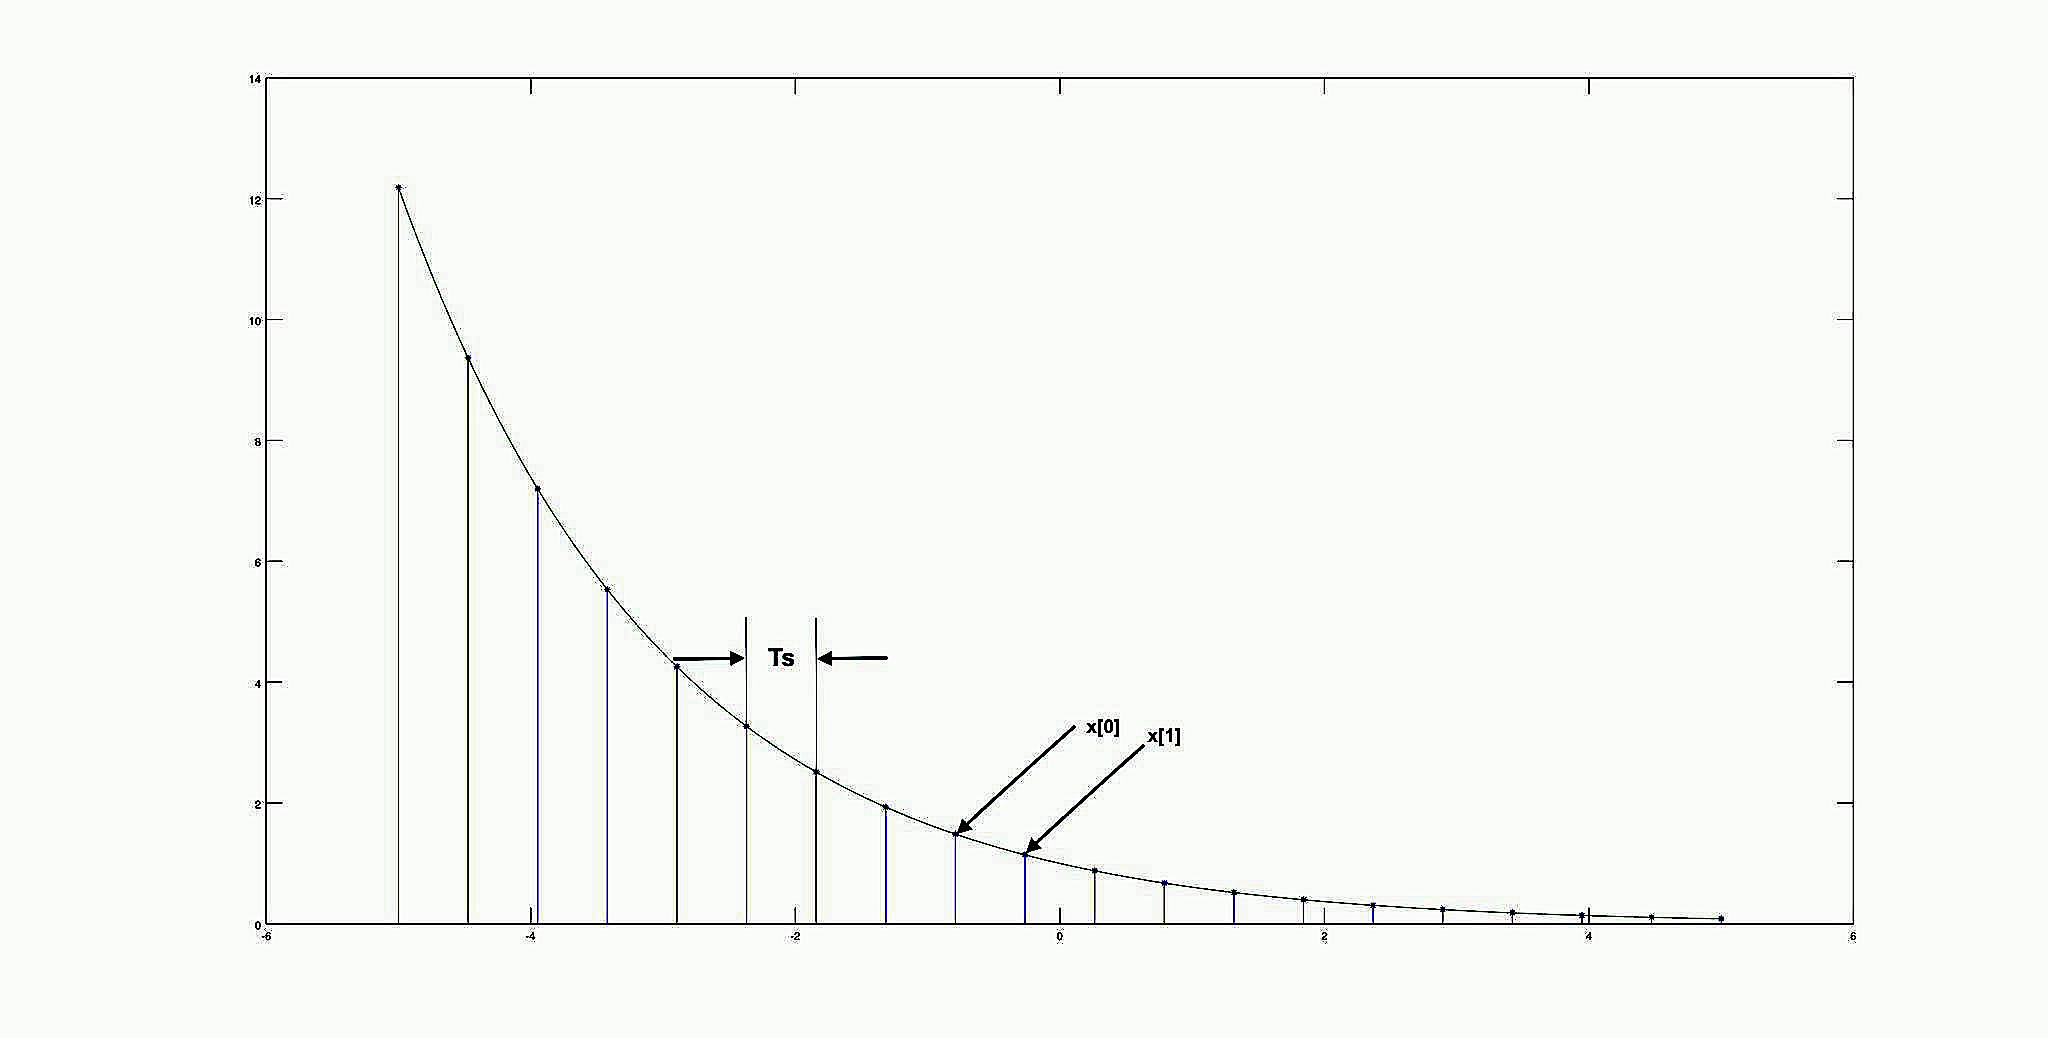
\includegraphics[width=\textwidth]{sampled.jpeg}
\end{figure}

In fig. 1, we see a continuous time signal $x(t)$ being sampled at a frequency of $1/T_{s}$ where $T_{s}$ is the length of the $sampling$ $interval$. The origin (the point $t=0$) of the resulting discrete signal can be assigned as per convenience.\\

We obtain, then, from the continuous signal, a discrete signal which, in some ways, is similar to the orignal continuous signal; it is a replica of the continuous signal. Music lovers might be like, ``Wait a minute! Aren't we loosing out on a lot of information in doing that? Won't my music sound bad?" We, however, resort to some clever techniques so that this loss is not perceptible to the human senses. And we can always resort to a higher sampling frequency. Thus, in the case of an audio CD, the sampling rate is 44,100 Hz i.e. we sample the audio signal 44,100 times in a second! We hope, thus, that we do not loose out a lot on the human experience of the music (or the image or video. Yes even the images we deal with these days are discretised. In what way do you think is this done?).\\

In this module, we set out to answer this basic about sampling a continuous time signal. We recognise that it is necessary and convenient to sample the signal as mentioned above. However,we must ask ourselves if the sampling we perform is even meaningful; meaningful in the sense that this sampling does not cost us a lot. We might loose information when sampling. Is this information loss tolerable or can we process the signals (both the sampled and the orignal) so that the result is acceptable. Or should we just increase the sampling frequency? While pondering over these, we must remember the enormous benefits sampling provides us. Thus it is a trade off and we would attempt to provide an analytical approach to solve this dilemma in the future lectures. While studying this, we explore the aforementioned connection between discrete and continuous signals and systems.

\subsection{A Priori Information}
When going from a continuous signal to a sampled version of it, we noted above that we might end up loosing some information contained in the orignal signal i.e. the signal reconstructed from the sampled signal may not resemble the orignal signal as much as we might want it to. The central idea in determining if this is the case, if reconstructing the original signal is simple or hard is the idea of apriori information. Apriori information is the information we have about the signal before we start the process of reconstruction. We illustrate this idea with a series of examples below.\\

\subsubsection{Some Examples}
\subsubsection{Some Easy Cases}
Consider a constant continuous signal $x(t) = \alpha, \alpha \in \mathbb{R}$. We ask the question in the context of this signal now. Can we sample and reconstruct this signal? If so, how do we go about doing this? If we have the a priori information that the signal is a constant signal, then we just need to know the value of $\alpha$ to have complete knowledge about the signal so that we can reconstruct it fully. This can be achieved by sampling the signal at just one value of $t$, say $t_{0}$. As $x(t_{0}) = \alpha$ we get the value of $\alpha$ as required.\\

Consider now the situation where we know beforehand that the signal under consideration is zero everywhere. Then, in order to reconstruct it, we need no samples at all. Even in the case of a non trivial signal like a sinusoid given by $x(t) =  5cos(4t+2)$, if know that the signal is $x(t) = 5cos(4t+2)$, we do not need any samples to reconstruct the signal.\\

These examples bring out an important idea. The more a priori information we have, the less is the amount of effort needed to sample and reconstruct the signal. 

\subsubsection{Reconstructing an Exponential Signal}
Consider the case where the a priori information we have is that the signal is an exponential signal. Thus the signal is of the form $x(t) = A_{0}e^{\alpha t}$. In order to sample and reconstruct this signal, we observe that we need two samples, say at times $t_{1}$ and $t_{2}$. The values of the samples will thus be $x(t_{1})$ and $x(t_{2})$ respectively. Then, we obtain the following two equations.
\begin{equation}
    x(t_{1}) = A_{0}e^{\alpha t_{1}}
\end{equation}

\begin{equation}
    x(t_{2}) = A_{0}e^{\alpha t_{2}}
\end{equation}

Dividing the $(1)$ by $(2)$ and taking the natural logarithm on both sides, we obtain
\[
    \alpha = \frac{ln(x(t_{2})) - ln(x(t_{1}))}{t_{2}-t_{1}}
\]

Substituting this value of $\alpha$ in $(1)$, we obtain,
\[
    A_{0} = x(t_{1})e^{-\alpha t_{1}}
\]

Thus, samples at two finite times enable us to reconstruct the signal entirely with the a priori infirmation we have.

\subsubsection{Making the Problem Harder: A Sum of Exponentials}
Suppose we just know that the signal is finite sum of exponentials. Thus, if $M \in \mathbb{Z}$, 

\[
    x(t) = A_{1}e^{\alpha_{1} t} + A_{2}e^{\alpha_{2} t} + ... + A_{M}e^{\alpha_{M} t}
\]

If $M$ is unknown too, this problem is very hard to solve. Thus, for the purposes of illustration, we assume that $M$ is known. In that case, we have $2M$ unknowns, $\alpha_{1}$, $\alpha_{2}$, ...,$\alpha_{M}$ and $A_{1}$, $A_{2}$, ..., $A_{M}$. Thus, we need $2M$ samples to be able to reconstruct the signal entirely. Let the samples be taken at times $t_{1}$, $t_{2}$, ..., $t_{2M}$. In this case, we get the following system of equations,
\begin{align*}
    A_{1}e^{\alpha_{1} t_{1}} + A_{2}e^{\alpha_{2} t_{1}} + ... + A_{M}e^{\alpha_{M} t_{1}} &= x(t_{1})\\
    A_{1}e^{\alpha_{1} t_{2}} + A_{2}e^{\alpha_{2} t_{2}} + ... + A_{M}e^{\alpha_{M} t_{2}} &= x(t_{2})\\
.\\.\\.\\
    A_{1}e^{\alpha_{1} t_{2M}} + A_{2}e^{\alpha_{2} t_{2M}} + ... + A_{M}e^{\alpha_{M} t_{2M}} &= x(t_{2M})\\
\end{align*}

As can be seen however, this system of equations is highly non-linear in the unknowns and hence it is not exactly clear how a solution might be obtained. At this stage, we simplify the problem further. We assume that $\alpha_{1}$, $\alpha_{2}$, ...,$\alpha_{M}$ are known. In this case, $M$ samples suffice and we get the following system of equations.

\begin{align*}
    A_{1}e^{\alpha_{1} t_{1}} + A_{2}e^{\alpha_{2} t_{1}} + ... + A_{M}e^{\alpha_{M} t_{1}} &= x(t_{1})\\
    A_{1}e^{\alpha_{1} t_{2}} + A_{2}e^{\alpha_{2} t_{2}} + ... + A_{M}e^{\alpha_{M} t_{2}} &= x(t_{2})\\
.\\.\\.\\
    A_{1}e^{\alpha_{1} t_{M}} + A_{2}e^{\alpha_{2} t_{M}} + ... + A_{M}e^{\alpha_{M} t_{M}} &= x(t_{M})\\
\end{align*}

Then, this is a system of linear equations in $A_{1}$, $A_{2}$, ..., $A_{M}$. The fact that this systems is obtained by sampling a sum of exponentials guarantees that the $M$ equations are all independent and that a solution exists. This solution is also easily computable.\\

One can also assume, however, that the $A_{1}$, $A_{2}$, ..., $A_{M}$ are known and that $\alpha_{1}$, $\alpha_{2}$, ..., $\alpha_{M}$ are unknowns. We get the same system of equations as in the previous case. How can one solve this system to obtain $\alpha_{1}$, $\alpha_{2}$, ..., $\alpha_{M}$? We leave this as an exercise to the students. 


\section{Lecture 2: Non-uniqueness due to sampling}

\subsection{Introduction}
In previous lecture, we used a-priori information for filling information between different samples. For example take a exponential signal $$x(t) = Ae^{\alpha t}$$ We can do a unique reconstruction by just doing two measurements and filling everything in between by using a priori information of $x(t)$. Here we will look at what happens when we don't have a-priori information for reconstruction. 

\subsection{Non-uniqueness due to lack of a-priori Information}

Let's sketch the reconstruction of $x(t)$ for two measurements $$x(t_{1})= Ae^{\alpha t_{1}}$$ $$x(t_{2})= Ae^{\alpha t_{2}}$$  and $t_{1}\neq t_{2}$. If we have a-priori form we can fill everything in between $t_{1}$ and $t_{2}$ and elsewhere using that information (black line in Figure \ref{fig:nonunique}). Now suppose we know the same samples $x(t_{1})$ and $x(t_{2})$ and a-priori form is not given, then how we will proceed with reconstruction. The problem is not that there are no possibilities but that there are too many of them. Some of them are shown in Figure \ref{fig:nonunique} along with the reconstruction when the given form is exponential. 

\begin{figure}[ht]
\centering
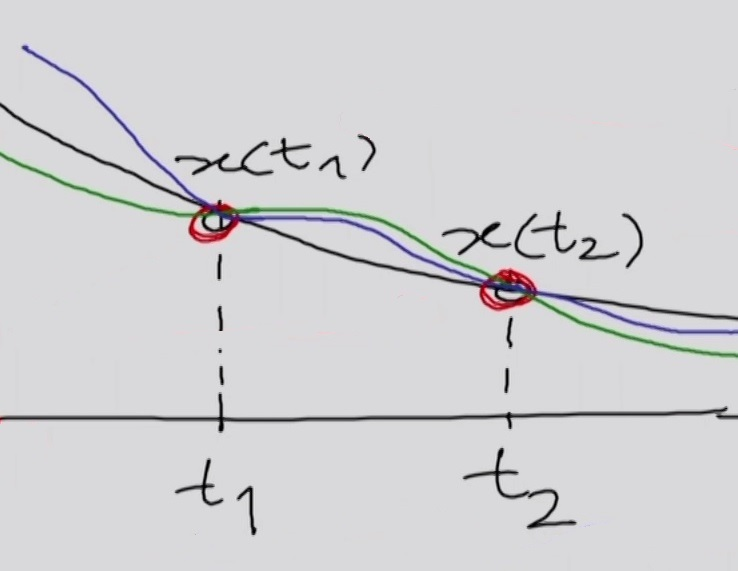
\includegraphics[width=0.7\textwidth]{nonunique.jpg}
\caption{\label{fig:nonunique}Non-unique reconstruction due to lack of a-priori Information}
\end{figure}

We can say the problem of sampling and reconstruction is similar to solving a crossword. We can think of clues as a-priori information and letters provided as samples.Without any a-priori information we can fill crossword any way we want but with clues we are restricted in our choice of filling up the crossword. Crosswords are generally designed such that there is a unique solution. Similarly in case of sampling and reconstruction a strong a-priori information restricts us to a unique reconstruction. 

\subsubsection{Degree of non-uniqueness in reconstruction}

When we know nothing about the form of signal then we see there is an infinity of possibilities. To answer how big is this infinity we must first see different classes of infinity. There is an infinity of natural numbers, infinity of integers, positive even/odd numbers etc. which are all same. Then there is an infinity of Real numbers which is bigger or higher than the infinity of integers in the sense that we can't put real numbers in one to one correspondence to integers without missing some real numbers. In case of reconstruction we need to define a value at every point. Some finite number of points have fixed value which are basically the samples but there is an infinity of points which don't have fixed value and can take any value in the absence of a-priori information. This infinity of possible reconstruction is thus even higher than infinity of real numbers. Now we can understand the degree of non-uniqueness of this problem.

How uniquely we can solve this problem of reconstruction depends on whether the given a-priori information completely complements the samples we have. We have previously seen that using Fourier transform we can represent a signal in terms of sinusoid. Let us take a sine wave and sample it and see what ambiguities we create. 

\subsection{Sampling Sinusoid}
Let us take a single sine wave and sample it uniformly i.e sampling with equal spacing between adjacent points. Now we need to find what are all sine waves which have these samples. The problem of ambiguity arises because we can miss an integer number of cycles between two samples. We can also arrive at a wrong edge. So with each possibility of losing a integer number of cycle one can also arrive at right edge or wrong edge. Let's analyse this mathematically bye taking $$A_{o}cos(\Omega _{o}t+\phi _{o})$$ as the form of sinusoid where $\Omega _{o}$ is the angular frequency and $T_{o}$ is the time period $$\Omega _{o}=\frac{2\pi }{T_{o}}$$ 

Now the process of sampling creates many 'ghost' or 'monster' frequencies which have the same samples at the same points. Let's denote these frequencies by $\Omega_{kj}$ where j($j = 1,2$) corresponds to two possibilities of correct or wrong edge. $$x(t) = A_{o}cos(\Omega _{kj}t+\phi _{kj})$$ $$k = 1,2,3,...$$ When $x(t)$ is sampled at time $nT_{s}$ where $n$ belongs to set of integers, we get $$x[nT_{s}]=A_{o}cos(\Omega _{o}nT_{s}+\phi _{o})$$ The non-uniqueness comes from being able to add a phase to this. Let's add $\pm 2\pi kn$ to the phase where $n$ is the sampling instant and $k$ belongs to set of positive integer. $$A_{o}cos(\Omega _{o}nT_{s}\pm 2\pi kn+\phi _{o})$$ $$=A_{o}cos(nT_{s}(\Omega _{o}\pm \frac{2\pi}{T_{s}}k)+\phi _{o})$$ $$=A_{o}cos(2 \pi nT_{s}(\frac{1}{T_{o}}\pm \frac{k}{T_{s}})+\phi _{o})$$ We need to have more than one sample in a cycle. We can see importance of this by taking a extreme example where we take just one sample per cycle and at the same location in every cycle. We will get same sample in every cycle. We cant even tell whether it is a DC or a sinusoid. Thus we can say that time interval between the samples must be less than cycle time.

$(\frac{1}{T_{o}}\pm \frac{k}{T_{s}})$ represents all possible Hertz frequencies. Let's take the possibility of $k=1$ $$(\frac{1}{T_{o}}-\frac{1}{T_{s}}) < 0$$ as $T_{s}<T_{o}$ but we don't want negative frequencies. Let's go back to original expression and see how we can correct this.$$A_{o}cos(2 \pi nT_{s}(\frac{1}{T_{o}}\pm \frac{k}{T_{s}})+\phi _{o})$$ $$=A_{o}cos\pm(2 \pi nT_{s}(\frac{1}{T_{o}}\pm \frac{k}{T_{s}})+\phi _{o})$$ If we take $+$ we get the same expression and if we take $-$ we get $$=A_{o}cos(-2 \pi nT_{s}(\mp\frac{k}{T_{s}}+ \frac{1}{T_{o}})-\phi _{o})$$ we see that the phase is reversed.

\subsubsection{Ghost Frequencies: An Example}
Let's take the case of $k=1$ again. Take $+$ for $(\frac{1}{T_{s}}+ \frac{1}{T_{o}})$ $$A_{o}cos(2 \pi nT_{s}(\frac{1}{T_{o}}+ \frac{1}{T_{s}})+\phi _{o})$$Take $-$ for $(-\frac{1}{T_{s}}+ \frac{1}{T_{o}})$ $$A_{o}cos(2 \pi nT_{s}(\frac{1}{T_{s}}- \frac{1}{T_{o}})-\phi _{o})$$

Take $T_{s}=\frac{T_{o}}{4}$ $$\frac{1}{T_{o}}+ \frac{1}{T_{s}} = \frac{5}{T_{o}}$$ $$\frac{1}{T_{s}}- \frac{1}{T_{o}} = \frac{3}{T_{o}}$$

Let's analyse this situation graphically. Take $T_{o}=\frac{\pi}{2}$
In Figure \ref{fig:sin} Black reconstruction is the true sinusoid and red is the sinusoid with ghost frequency $ = \frac{5}{T_{o}}$

\newpage

\begin{figure}[ht]
\centering
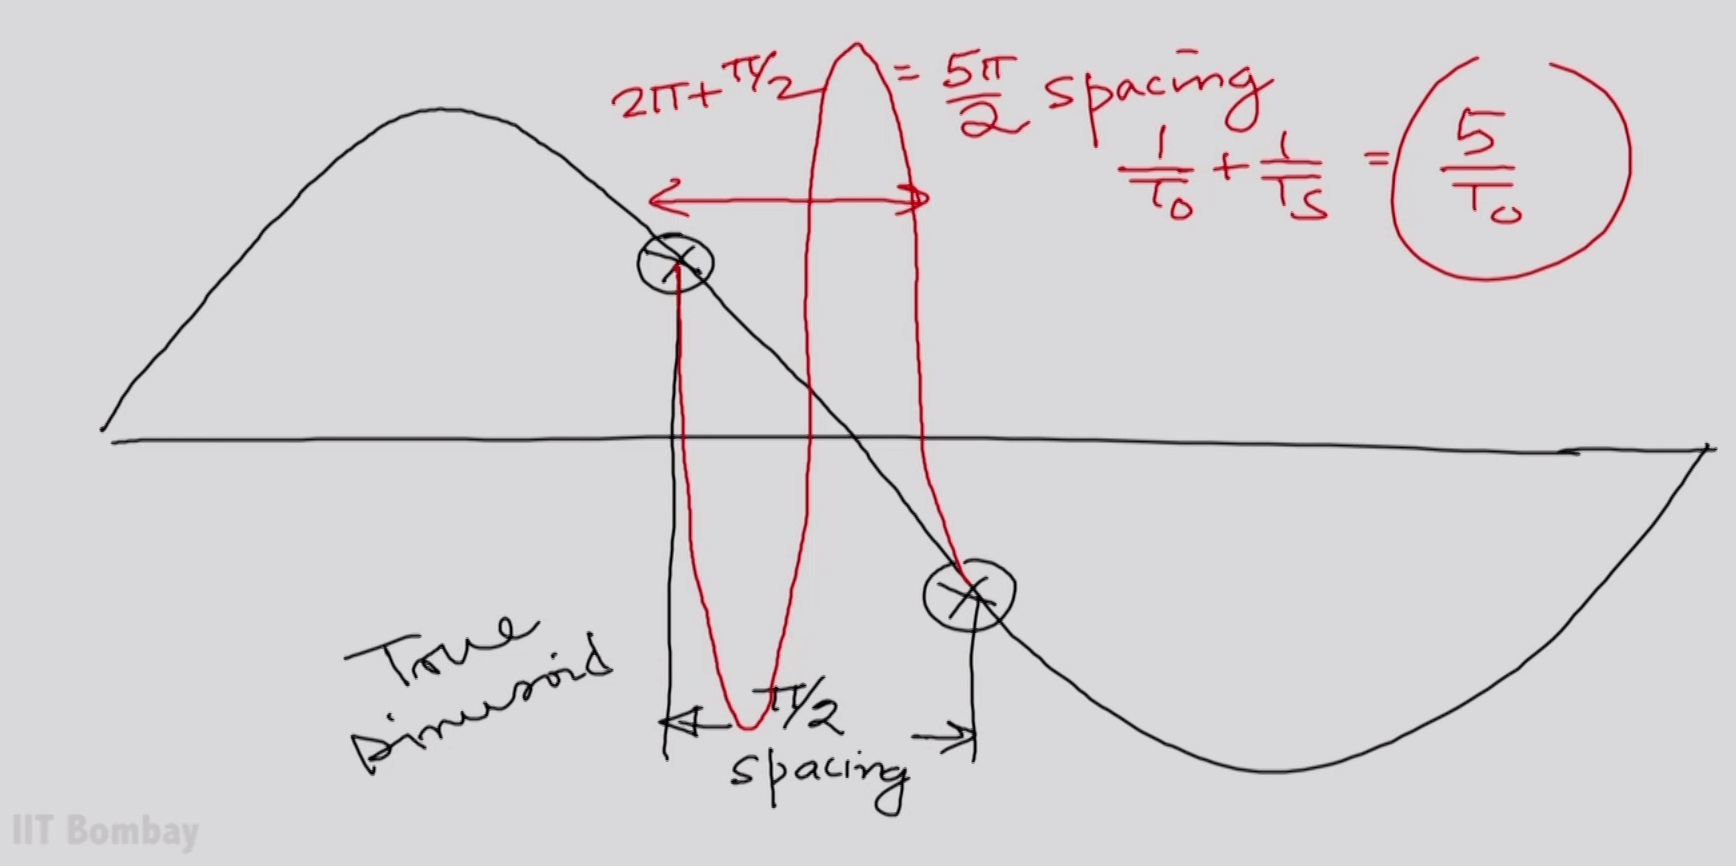
\includegraphics[width=1\textwidth]{sin.jpg}
\caption{\label{fig:sin}True sinusoid and Ghost frequencies}
\end{figure}

Exercise : Draw the sinusoid when you almost miss the cycle and arrive on the wrong edge and verify the ghost frequency $ = \frac{3}{T_{o}}$ and the spacing to be $\frac{3\pi}{2}$


\section{Lecture 3: Concept and expression of Impostor Terms}

\subsection{Introduction}
Previously, we have talked about ``sampling'' signals, that is, you only ``read'' and ``store'' the value of the signal at certain points. We saw the problems associated with sampling, mainly the fact that given just the sampled signal, it is not possible to reconstruct the original signal, because there are many possible signals which would have given the \emph{same} samples, i.e. they would have taken on the same values as this signal at the points where we are sampling. The natural question to ask, then, is what ``extra information'' do we need in order to reconstruct the original signal from this sample? To do that, we first have to know what these ``other signals'' look like.

\subsection{Non-Uniqueness of Samples}

Previously, we saw graphically that many different sinusoids can have the same samples. We'll now do essentially the same thing, algebraically.

A sinusoid, in general, is of the form $A_0\cos(\Omega_0 t +\phi_0)$, where $\Omega_0 = \frac{2\pi}{T}$, $T$ being the time period, and $\phi_0$ is the initial phase.

Now we saw that the process of sampling was also creating ``ghost frequencies'', frequencies different from that of the original signal, as a side-effect. Of course, these ``impostor terms'', as we can call them, have the same values as the original signal at the point of sampling. We also saw how you can lose a full cycle and arrive at the correct edge, or you only lose half a cycle and arrive at the wrong edge.

Let us represent these ``monster frequencies'' as 
\begin{equation}
\label{eqn:rep}
A_0\cos(\Omega_{kj} t +\phi_{kj})
\end{equation}
Here, $k$ is the number of cycles lost (including the half cycles, if any). $j=1$ signifies that you arrived at the correct edge, and $j=2$ stands for arriving at the wrong edge.

Now suppose we uniformly sample the signal at points $t=nT_s$. We have:
\[x(nT_s)=A_0\cos(\Omega_0 n T_s +\phi_0)\]
Because of the periodicity of the cosine, we can add $\pm 2\pi n k$ to the phase without changing the value of the expression.
\[x(nT_s)=A_0\cos(\Omega_0 n T_s \pm 2\pi nk +\phi_0)
=A_0\cos\left\{2\pi n T_s \left(\frac{1}{T_0} \pm \frac{k}{T_s}\right) +\phi_0\right\}\]
Here, one can think of the term $\frac{1}{T_0}\pm\frac{k}{T_s}$ as the frequency of the impostor in cycles/second, where $k\in \mathbb{Z}^+$.

Now let us assume, for the time being, that we are sampling the sinusoid at least one in each cycle. This is a very reasonable assumption, because if you take less than one sample per cycle, your original sinusoid is itself completing a whole cycle before the next sample is taken. Thus, we assume that $T_0 > T_s$.This would imply that $\frac{1}{T_0}-\frac{k}{T_s}<0$, which says that the frequency is negative, which is something we don't like! But that's not too bad! We know that $\cos$ is symmetric about the $y$-axis. Hence, instead of only one expression with the $\pm$, we write two separate expressions:

\[A_0\cos\left\{2\pi n T_s \left(\frac{1}{T_0} + \frac{k}{T_s}\right) +\phi_0\right\}\]

\centerline{and}

\[A_0\cos\left\{-\left\{2\pi n T_s \left(\frac{1}{T_0} - \frac{k}{T_s}\right) +\phi_0\right\}\right\}=
A_0\cos\left\{2\pi n T_s \left(\frac{k}{T_s}-\frac{1}{T_0}\right) - \phi_0\right\}
\]

Here, the first expression represents that we arrived on the correct edge after skipping $k$ cycles completely, and the second one means that we arrived at the incorrect edge after ``almost'' skipping $k$ cycles. Hence, with respect to the expression (\ref{eqn:rep}) which we wrote earlier, we can say that
\begin{align}
\Omega_{k1}&=2\pi\left(\frac{k}{T_s} + \frac{1}{T_0}\right)  &\phi_{k1}=\phi_0\\
\Omega_{k2}&=2\pi\left(\frac{k}{T_s} - \frac{1}{T_0}\right) &\phi_{k2}=-\phi_0
\end{align}
It is worthwhile to note that the signs of $\frac{1}{T_0}$ and $\phi_0$ match in both expressions.

\begin{figure}[ht]
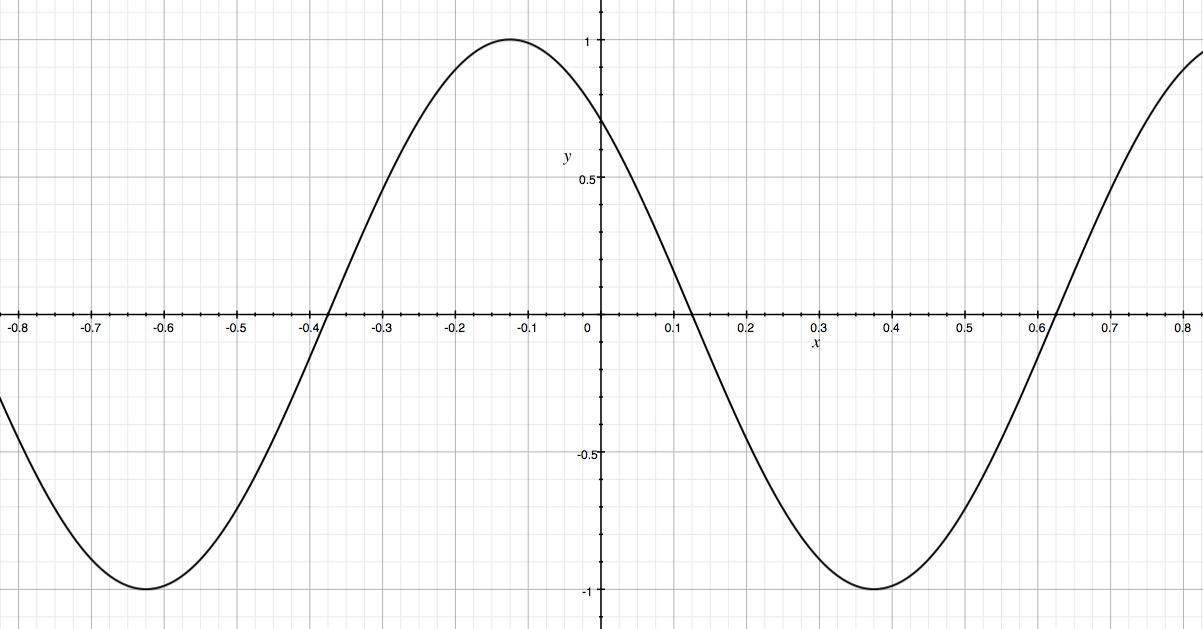
\includegraphics[width=\textwidth]{1-Original}
\caption{\label{fig:1}The original signal, $y=\sin\left(\frac{2\pi t}{T_0}+\frac{\pi}{4}\right)$}
\end{figure}

\begin{figure}[ht]
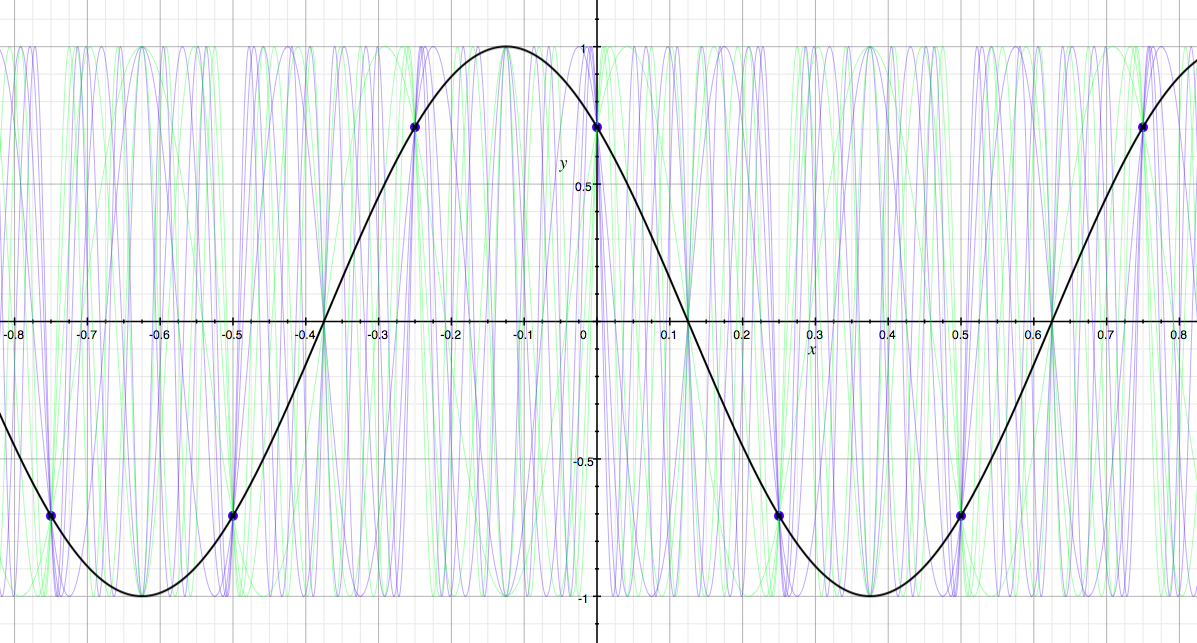
\includegraphics[width=\textwidth]{2-Sampled}
\caption{\label{fig:2}The original signal, from Figure~\ref{fig:1}, sampled at points $t=nT_s , \forall n\in\mathbb{Z}$}
\end{figure}

\begin{figure}[ht]
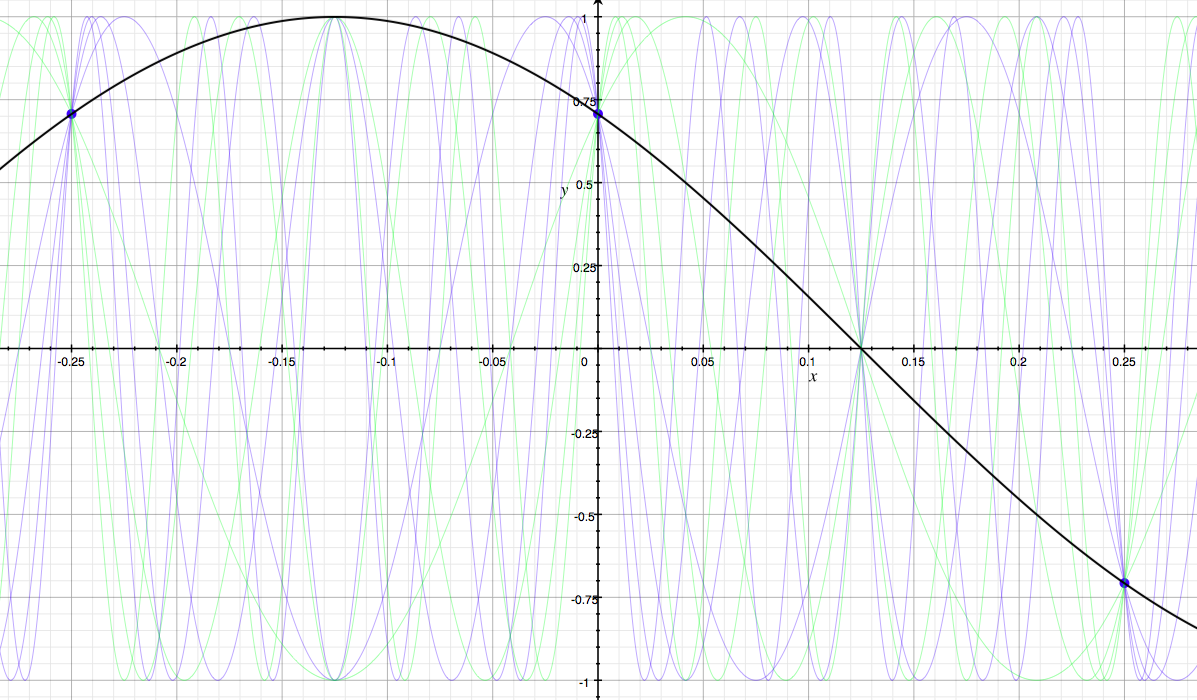
\includegraphics[width=\textwidth]{3-Zoomed_In}
\caption{\label{fig:3}Zoomed in view of the same signal}
\end{figure}

\begin{figure}[ht]
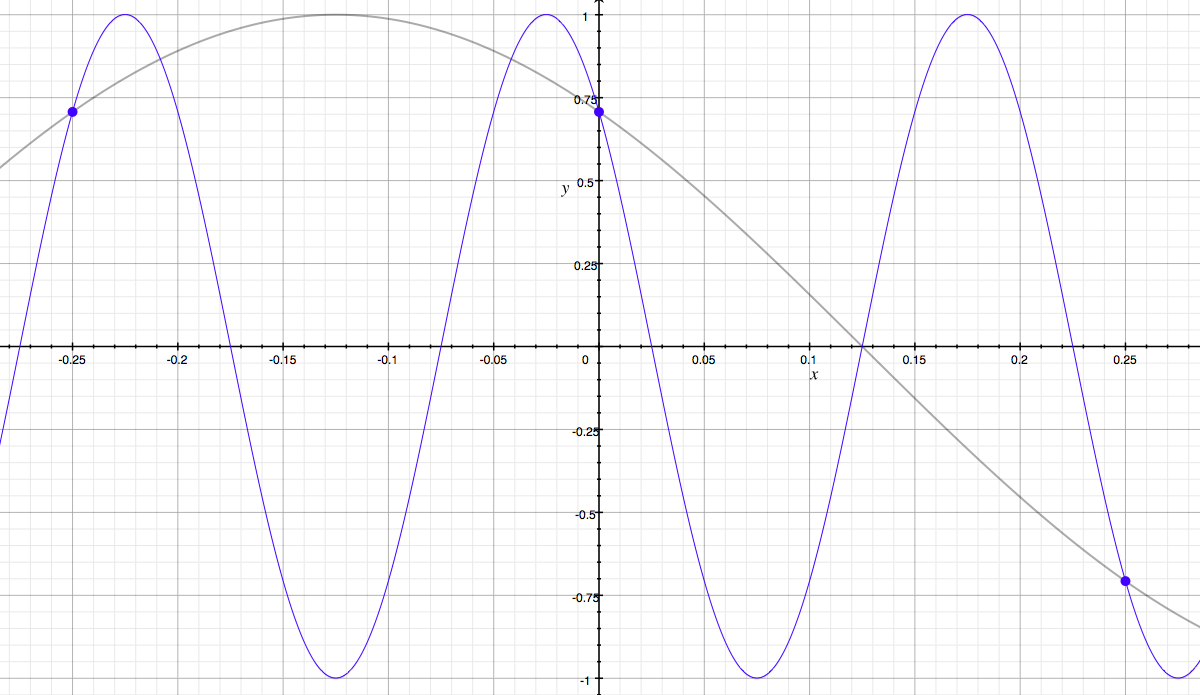
\includegraphics[width=\textwidth]{4-1CE}
\caption{\label{fig:4}Missing 1 cycle and arriving at the correct edge}
\end{figure}

\begin{figure}[ht]
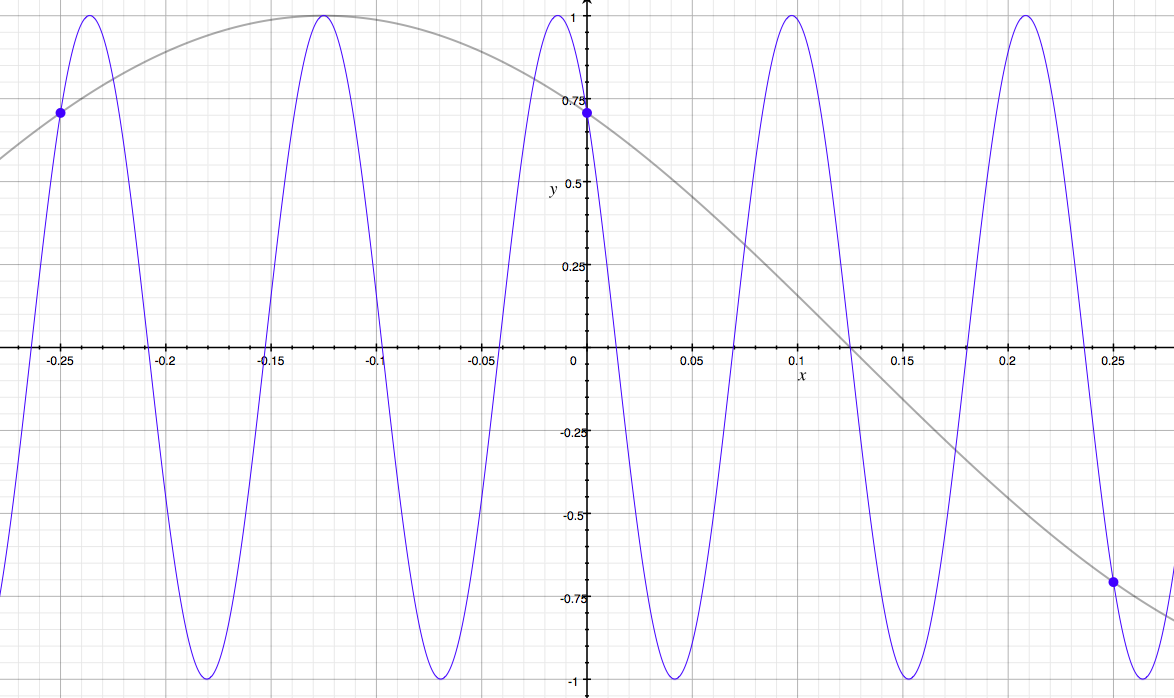
\includegraphics[width=\textwidth]{5-2CE}
\caption{\label{fig:5}Missing 2 cycles and arriving at the correct edge}
\end{figure}

\begin{figure}[ht]
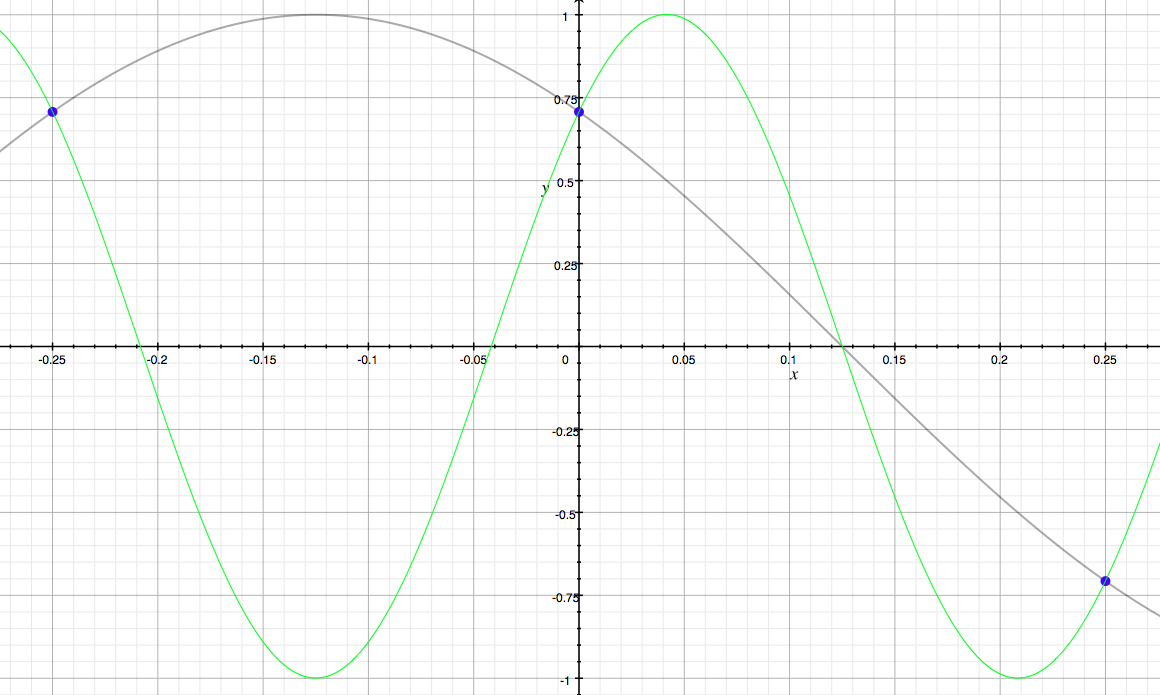
\includegraphics[width=\textwidth]{6-1IE}
\caption{\label{fig:6}Missing 1 cycle and arriving at the incorrect edge}
\end{figure}

\begin{figure}[ht]
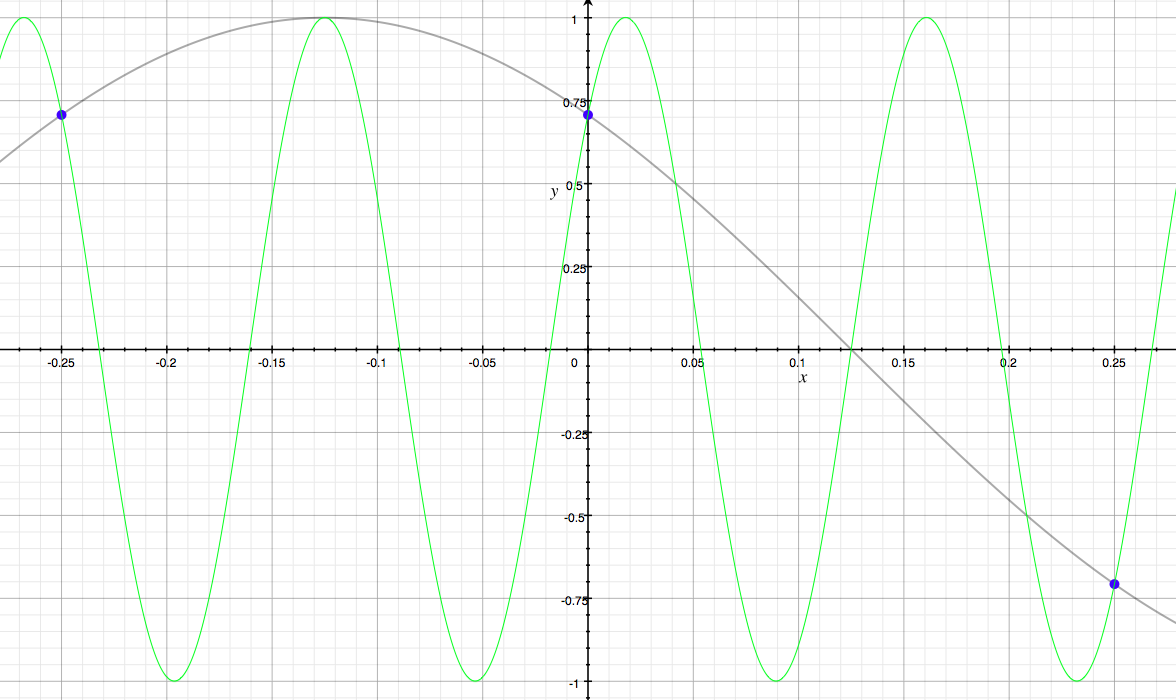
\includegraphics[width=\textwidth]{7-2IE}
\caption{\label{fig:7}Missing 2 cycles and arriving at the incorrect edge}
\end{figure}


\section{Lecture 4: Understanding the Impostor Terms}

\subsection{Introduction}
We have talked about how sampling a signal can create impostor terms. As discussed previously, these impostor terms have the same values at the sampled points, but are in essence different signals all together. We also looked at the impostor terms for when the original signal is a sinusoid and the impostor terms are also sinusoids. In this lecture, we will carry this discussion forward and see how the different sinusoids act all together.

\subsection{Adding the sinusoid terms}
\noindent Recall that the sinusoid terms can be written as follows:-
\[
A_{0} \cos \left (2\pi(\frac{k}{T_{s}}-\frac{1}{T_{0}})t - \frac{\pi}{4}\right)
\]
\[
A_{0} \cos \left (2\pi(\frac{k}{T_{s}}+\frac{1}{T_{0}})t + \frac{\pi}{4}\right)
\]

\noindent where k is any positive integer.

\noindent A sum of the original signal and all the impostor terms will look like:-

\[
A_{0} \cos \left (2\frac{\pi}{T_{0}}t+\frac{\pi}{4}\right) + \sum_{k=1}^{N}\left( A_{0} \cos \left (2\pi(\frac{k}{T_{s}}-\frac{1}{T_{0}})t - \frac{\pi}{4}\right)+ A_{0} \cos \left (2\pi(\frac{k}{T_{s}}+\frac{1}{T_{0}})t + \frac{\pi}{4}\right)\right)
\]
where N \textgreater 0
\\
At this point, the following substitution will make it easier to work out the math.
\[
B=\frac{2\pi k}{T_{s}}
\ and
\
C=\frac{1}{T_{0}} + \frac{\pi}{4}
\]
 Notice that the term C is independent of k.
 For a given k, the sum inside the $\Sigma$ reduces to 
\[ A_{0}\cos (B-C) + A_{0}\cos (B+C) = 2A_{0}\cos B\cos C
\]
This will make the sum :-

\[
A_{0} \cos \left (2\frac{\pi}{T_{0}}t+\frac{\pi}{4}\right) + \sum_{k=1}^{N}\left( 2 A_{0} \cos \left (2\frac{\pi}{T_{0}}t+\frac{\pi}{4}\right) \cos \left( \frac{2\pi k}{T_{s}}\right)\right)
\]
which can be further computed as:-
\[
A_{0} \cos (C) + \sum_{k=1}^{N}\left( 2A_{0} \cos  (C) \cos (B)\right)
\]
\[
A_{0}\cos C \lbrace 1 + 2\sum_{k=1}^{N} \cos B \rbrace
\]
Using the polar representation of $\cos \theta$, we can refine the sum in the brackets to be:-
\[
\lbrace 1+ \sum_{k=1}^{N} \left( exp(\frac{j 2 \pi k t }{T_{s}}) + exp(\frac{-j 2 \pi k t }{T_{s}})  \right)
\]
which can also be written as:-
\[
1+2\;\sum_{k=1}^{\infty} \cos (\frac{2\pi}{T_{s}}kt)
\]
Keep this in mind because we will later draw a similar conclusion from a quite different manipulation.
\noindent Note that the individual terms of the sum of exponentials can be added using the series for a Geometric progression quite easily. The first few steps are as follows:-
\[
\sum_{k=1}^{N} \left( exp(\frac{j 2 \pi k t }{T_{s}}) \right) = exp(\frac{j2\pi t}{T_{s}})\left( \frac{1-exp(\frac{j2\pi t}{T_{s}} (N+1))}{1-exp(\frac{j2\pi t}{T_{s}})}\right) 
\]
\[
=exp(\frac{j2\pi t}{T_{s}}) \left( exp\middle ((\frac{j2\pi t}{T_{s}})(\frac{N+1}{2})\middle) \times  \middle( 2j\sin\middle((\frac{j2\pi t}{T_{s}})(\frac{N+1}{2})\middle)\right)\]\[ \div\]\[ \left( exp\middle ((\frac{j2\pi }{T_{s}})(\frac{t}{2})\middle) \times  \middle( 2j\sin\middle((\frac{j2\pi }{T_{s}})(\frac{t}{2})\middle)\right)
\]

The following are left as exercises to the reader:-
\begin{itemize}
\item Sketching this function as a function of $t$ after further simplification and arithmetic .
\item Analysis of the function for when $N$ grows.
\item Analysis of the function for when $t=nT_{s}$ and when $t \neq nT_{s}$
\item Proceeding similarly for the other term in the original sum i.e. $ exp(\frac{-j 2 \pi k t }{T_{s}})$ and conducting the same analysis for the resultant function.
\end{itemize}


\subsection{An Alternate Path - By Sampling}

\noindent The previous section contained a lot of mathematical computations with a large number of terms. We would like to tackle the problem in an alternate way which doesn't involve such heavy algebra.
\newline
Such an alternate way is to proceed by actually sampling the signal. By sampling the signal, we mean that the signal is retained around the sampling times $(nt_{s})$ for a time period of $\Delta$; i.e. the width of the signal is $\Delta$.
\begin{figure}[h]
\centering
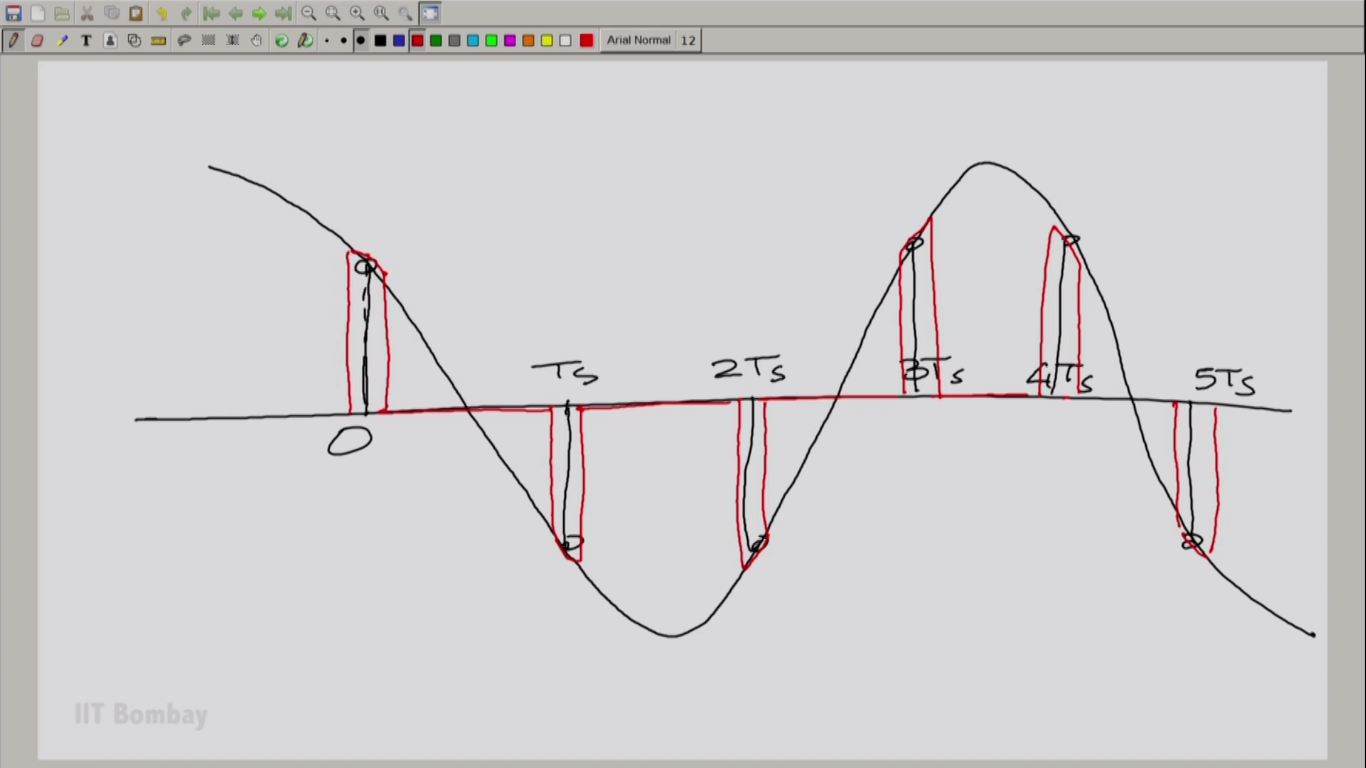
\includegraphics[scale=0.25]{curve.png}
\caption{The red curve represents the sampled signal while the black curve represents the original signal}
\end{figure}

\noindent The sampled curve can also be seen as the multiplication of the original signal (the sinusoid) with a train of very narrow pulses with unit height. However, note that these pulses are not impulses because they have a finite height (unit in this case).
\newline
Also note that this train of impulses is an even periodic function and hence, will have a Fourier series expansion of the form:-
\[
c_{0}+ \sum_{k=1}^{\infty} c_{k} \cos (\frac{2\pi}{T_{s}}kt + 0)
\]
The phase is $0$ because the function is even. $k=1$ represents the "fundamental" while $k$ \textgreater $1$ represents the "harmonics".
\newline
Using the previously learnt methods of computing the Fourier coefficients, 
\[
c_{0}=\frac{1\cdot \Delta}{T_{s}}
\]
and
\[
c_{k}=\frac{2}{T_{s}} \int \limits_{\frac{-\Delta}{2}}^{\frac{\Delta}{2}} 1 \cdot \cos (\frac{2\pi}{T_{s}}kt) dt
\]
\[
=\left.\frac{2}{T_{s}} \frac{\sin (\frac{2\pi}{T_{s}}kt)}{(\frac{2\pi}{T_{s}}k)} \right|_{\frac{-\Delta}{2}}^{\frac{\Delta}{2}}
\]
On substituting the limits and simplifying the value,
\[
c_{k}=\frac{2}{k} \sin (\frac{k\pi \Delta}{T_{s}})
\]
We see that the Fourier series becomes trivial for when $\Delta \rightarrow 0 $. To prevent this, we employ the same technique as we did in Module 1, we modify the pulse in such a way that the height is the inverse of the width. Note that this had converted our $pulse$ to an $impulse$.
\newline
The Fourier coefficients now become,
\[
c_{k}=\frac{1}{T_{s}}\cdot\frac{2}{\frac{k\Delta}{T_{s}}} \sin (\frac{k\pi \Delta}{T_{s}})
\]
Now, the Fourier expansion doesn't become trivial when $\Delta \rightarrow 0$. Rather, we can see that this is nothing but the sinc function.
\newline
Hence, we can see that 
\[
c_{k} \rightarrow \frac{2\pi}{T_{s}} \;\;\;\; as \;\;\;\; \Delta \rightarrow 0
\]

\subsection {Another Way of Sampling}
We can also write the complex Fourier expansion of the train of impulses. And proceed to multiply the original signal by the Fourier expansion (complex expansion) of the train of impulses. This is different from our previous method in the aspect that we have started with a train of impulses straightaway; instead of considering pulses and then converting them to impulses. This will give us the same result.
\newline
The complex Fourier expansion of this train of impulses is as follows; where $\gamma _{l}$ are the coefficients of each term of the expansion
\[
f(t)=\sum_{l=-\infty}^{\infty} \gamma_{l} \cdot exp(j \frac{2\pi}{T_{s}}lt)
\]
where f(t) is the train of impulses.
\newline
Let p(t) denote any one of the impulses which are periodically repeated over the entire $x$-axis to get f(t). Then for finding $\gamma_{l}$  :-
\[
\gamma_{l}= \frac{1}{T_{s}}\;\int \limits_{-\frac{T_{s}}{2}}^{\frac{T_{s}}{2}} \left( p(t)\cdot exp(-j \frac{2\pi}{T_{s}}lt) \right)  \; dt
\]
By the sifting property of the impulse, we can show that :-
\[
\gamma_{l}=\frac{1}{T_{s}}
\]
Hence, the complex Fourier expansion of the train of impulses is:-
\[
f(t)=\frac{1}{T_{s}}\;\sum_{l=-\infty}^{\infty} exp(j \frac{2\pi}{T_{s}}lt)
\]
which can further be simplified by taking the term for $l=0$ out of the sum and clubbing the terms with the same value of l, but with different signs together:-
\[
f(t)=\frac{1}{T_{s}}+\frac{1}{T_{s}}\;\sum_{l=1}^{\infty} exp(j \frac{2\pi}{T_{s}}lt) + exp(-j \frac{2\pi}{T_{s}}lt)
\]
This can be further simplified as:-
\[
f(t)=\frac{1}{T_{s}}+\frac{2}{T_{s}}\;\sum_{l=1}^{\infty} \cos (\frac{2\pi}{T_{s}}lt)
\]
This is the same as what we saw when we added all the impostor terms together!
\subsection{Conclusions}
We took two paths to analysing the imposter terms and the original sinusoid; the first was adding all these terms while the second was sampling the signal using impulses and analysing the resultant signal. For the analysis with impulses, we took two ways; the real Fourier series and the complex Fourier series expansions of the train of impulses.
\newline
Our observation is that both these processes are in fact, the same!
\newline
So, to conclude, bringing all these "impostor" sinusoids together with the original amounts to multiplying the original sinusoid with a uniform train of impulses located at the sampling instants!
\newline
Another indirect observation is that since the addition of all the impostor sinusoids with the original is the same as the sampling of the original sinusoid, they have constructive interference at the sampling instants (and hence return a finite value) and have a destructive interference everywhere else (hence the curve vanishes everywhere else).
\newline
These conclusions should be kept in mind as they are essential to the development of concepts that will be introduced further.


\section{Lecture 5: Sampling of signals having Fourier Transform}


\subsection{Sampling}

Ideal sampling is multiplication of the waveform by a uniform train of impulses located at sampling instants.
If $x(t)$ is being sampled, we are multiplying $x(t)$ with $p(t)$ which has impulses located at every sampling instants.
$p(t)$ is shown below.

$$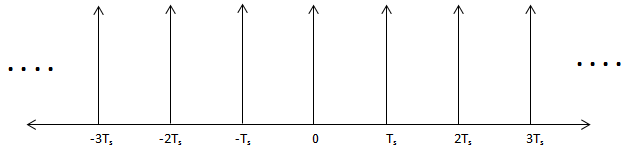
\includegraphics[width=0.5\textwidth]{p_t_.png}$$


Altrnately, we are multiplying original function $x(t)$ by complex fourier expansion of the uniform impulse train.

\subsubsection{Sampling of sinusoid}

Let us focus on one constituent component, or sinusoid in the original waveform $$A_0  \cos ( \frac{2 \pi t}{T_0} + \phi _0 ) $$
Now we are generalizing it to any phase $\phi_0$ unlike we took $\frac{\pi}{4}$ in previous lecture. (Any  $\phi_0 $ will do)

Ideal sampling results in this becoming,
$$ K_0  \left\{ A_0  \cos ( \frac{2 \pi t}{T_0} + \phi _0 )   + \sum_{l=1}^\infty  \left\{  A_0  \cos \left[2\pi(\frac{l}{T_s}-\frac{1}{T_0})t - \phi _0 \right]  +  A_0  \cos \left[2\pi(\frac{l}{T_s}+\frac{1}{T_0})t + \phi _0 \right] \right\} \right\} $$
where $K_0$ is some constant depends on the strength of the impulses.
We have to make sure that all these frequencies are distinct i.e, the imposters do not overlap on original frequencies.As long as $\frac{1}{T_0}$much less than$\frac{1}{T_s}$, all these are distinct frequencies.

Example:  $\frac{1}{T_0} = 1   \mbox{ khz}$, $\frac{1}{T_s} = 20   \mbox{ khz}$
  
  The frequencies are $$\frac{1}{T_0},(\frac{1}{T_s} - \frac{1}{T_0} ),(\frac{1}{T_s} + \frac{1}{T_0}),(\frac{2}{T_s} - \frac{1}{T_0} ),(\frac{2}{T_s} + \frac{1}{T_0})...$$
  
   The frequencies are $ 1,19,21,39,41,...$.Clearly they are distinct!

How small can $\frac{1}{T_s}$ be to keep the frequencies distinct ?
\subsubsection{Keeping imposters distinct}

We are keen on the frequencies being distint because imposters should be distingushable from original waveform.
$$(\frac{1}{T_s} - \frac{1}{T_0} )<(\frac{1}{T_s} + \frac{1}{T_0})$$
We are doubtful if $\frac{1}{T_0}$ and $\frac{1}{T_s} - \frac{1}{T_0}$ are distinct.They are distinct if

 $$(\frac{1}{T_s} -\frac{1}{T_0} )> \frac{1}{T_0}$$
$$\frac{1}{T_s}>\frac{2}{T_0}$$


So,any sampling rate$\frac{1}{T_s}$ greater than(STRICTLY GREATER) twice of original frequency$\frac{1}{T_0}$.That means $\frac{1}{T_s}=3 \mbox{ khz}$ is enough. No need of taking samples at $20 \mbox{ khz}$ frequency.For sampling rate$\frac{1}{T_s}$ the frequencies are $1,2,4,5,7,8,10$.Notice they are still distinct. 

Also note $$\frac{1}{T_s} \neq 2 \mbox{ khz}$$ as $1^{st}$ imposter sits on original waveform.

\subsection{Signals which have and do not have a Fourier transform} 
A waveform or signal is comprised of many sinusoids, the FT of the signal may contain discrete frequencies ( case where $x(t)$ is periodic ), or there can be continuum of frequencies ( when $x(t)$ is aperiodic ).

When we say a waveform is composed of many constituents, we say that waveform has fourier transform.
\subsubsection{Signal having Fourier Transform}

An example of signal that has fourier transform :-

$x(t)=e^{-t}u(t),  
u(t)=$standard unit step



$$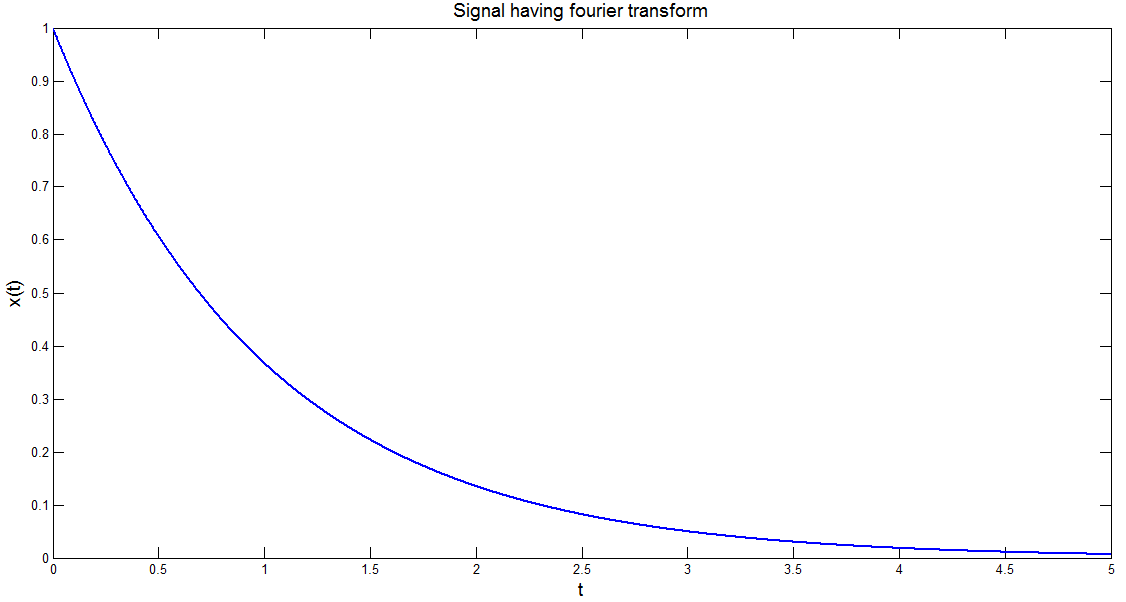
\includegraphics[width=0.6\textwidth]{e_-t.png}$$



$$X(\Omega)= \int_{-\infty}^{+\infty} x(t)e^{-j\Omega t}\mbox{dt}=\int_{-\infty}^{+\infty} e^{-t}e^{-j\Omega t}\mbox{dt}= \int_{-\infty}^{+\infty} e^{-(1+j\Omega t)}\mbox{dt}= \frac{1}{1+j\Omega}$$


$$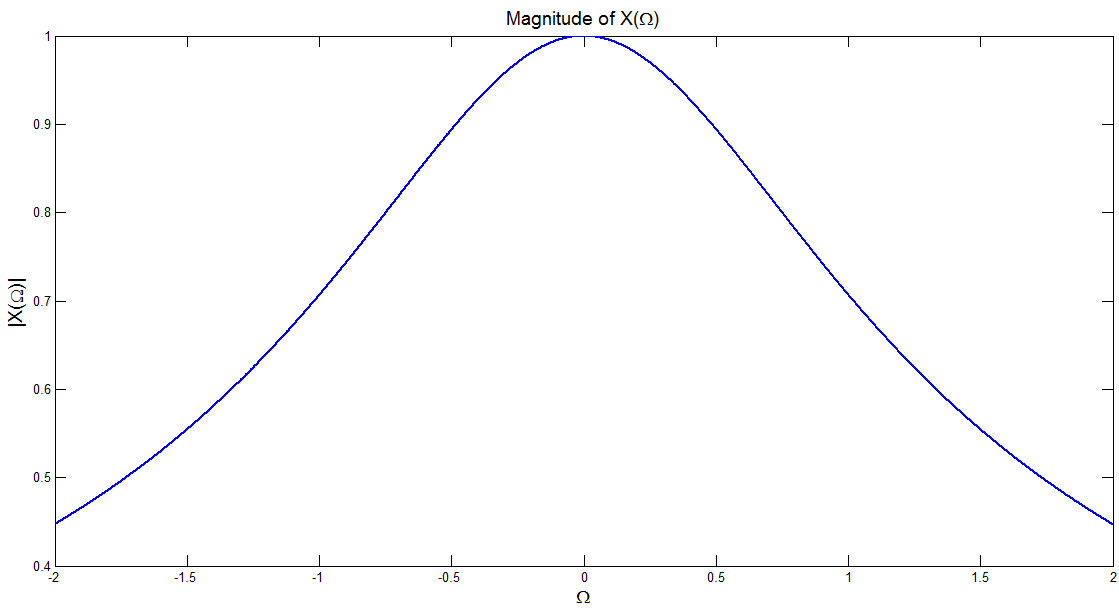
\includegraphics[width=0.6\textwidth]{_X_f__.png}$$

$$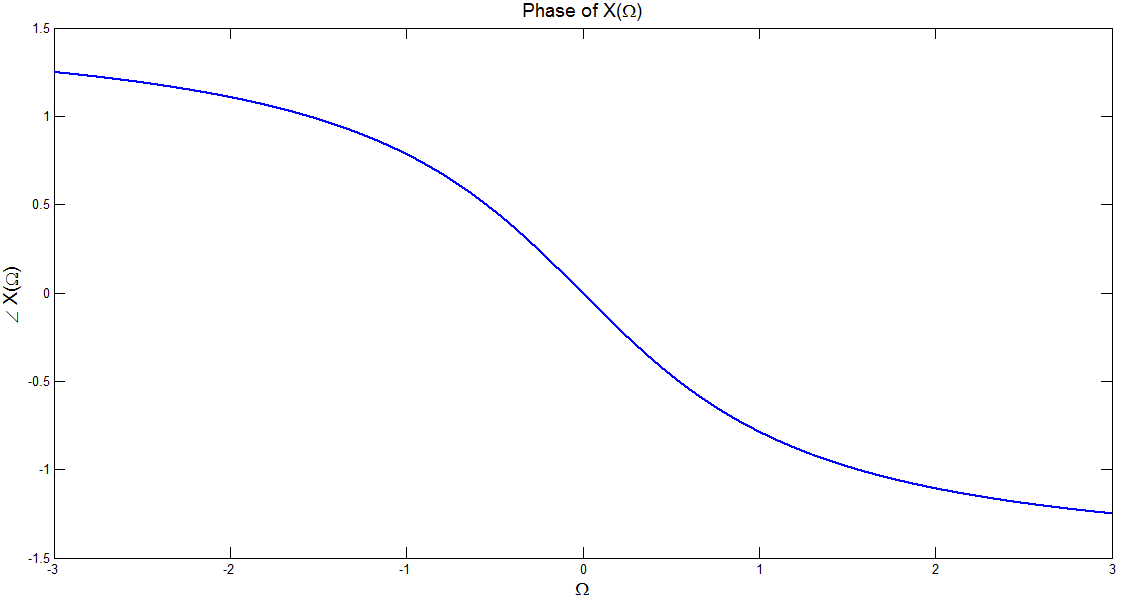
\includegraphics[width=0.6\textwidth]{_lt_X_f_.png}$$


\subsubsection{Signals not having Fourier Transform}

An example for signal which does not have a fourier transform:- 
$y(t)=e^t u(t)$.



$$X(\Omega)= \int_{-\infty}^{+\infty} y(t)e^{-j\Omega t}\mbox{dt}=\int_{-\infty}^{+\infty} e^{t}e^{-j\Omega t}\mbox{dt}$$
$$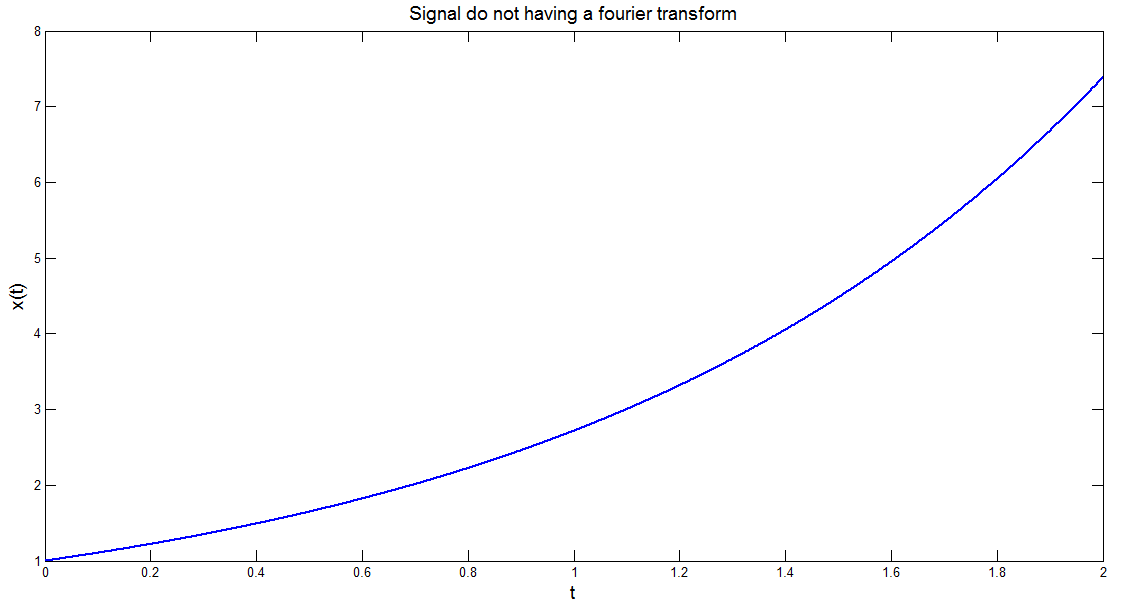
\includegraphics[width=0.6\textwidth]{e_t.png}$$
Clearly the integral doesnot converge.This signal is divergent and so no fourier transform.
Throughout the dicussion on sampling we omit signals which do not have fourier transform from consideration.We only focus on signal having Fourier transform.


$$x(t)=e^{-t}u(t) \iff X(\Omega)=\frac{1}{1+j\Omega}$$

We can reconstruct $x(t)$ from $x(\Omega)$

$$x(t)= \int_{-\infty}^{+\infty} X(\Omega)e^{j\Omega t}\mbox{d}\Omega$$

Recall in the geometric interpretation $X(\Omega)$ is component, $e^{j\Omega t}$ is vector, $\mbox{d}\Omega$ is aggregated over all vector and $\frac{1}{2\pi}$normalizes.

$$X(\Omega)= \overline{X(-\Omega)}$$ $$|X(\Omega)|=|X(-\Omega)|$$
$$ \angle X(\Omega)= - \angle X(-\Omega)$$

Consider  $X(\Omega)e^{j\Omega t} + X(-\Omega)e^{-j\Omega t}$, as one of the constituent.On expansion
$$|X(\Omega)| e ^{j\angle x(\Omega)} e^{j\Omega t} + |X(-\Omega)| e ^{j\angle X(-\Omega)} e^{-j\Omega t}  = 2|x(\Omega)|\{cos(\Omega t + \angle x(\Omega))\mbox{d}\Omega$$ .


We have continuum of such constituents ( $\Omega$ from 0 to $\infty$).



$x(t)$ is combination of $2|X(\Omega)|\{cos(\Omega t + \angle x(\Omega))\}$ for all  $\Omega$.
$$x(t)=\int_0^{\infty}\frac{2}{\sqrt{1+\Omega ^2}}\cos(\Omega t - \tan^{-1}\Omega)$$Note that for every $\Omega \neq 0$, we designed our constituent as combination of $\Omega$ and $-\Omega$ terms. Hence limits vary from $0$ to $\infty$.
Now, when we sample $x(t)$ each and every such constituent is sampled and creates its own imposters.Can we keep all those imposters distinct from original frequencies ? Can we ever sample "adequately" so that we can distinguish imposters from original frequencies?
\subsection{Linearity of sampling}
Recall constituent frequency $\frac{1}{T_0}$, sampling frquency $\frac{1}{T_s}$. Frequencies created in sampling are $$\frac{1}{T_0},\frac{1}{T_s}-\frac{1}{T_0},\frac{1}{T_s}+\frac{1}{T_0} ,\frac{2}{T_s}-\frac{1}{T_0},\frac{2}{T_s}+\frac{1}{T_0} , \cdots$$

The smallest $\frac{1}{T_s}$ we could use is $> \frac{2}{T_0}$ where $\frac{1}{T_0}$ was frequency of one constituent.

When we have combination of sinusoids, can we generalize constituent role ? 
Here a basic question arises: IS SAMPLING LINEAR?

Yes.
Sampling ideally means multiplying the signal by a uniform train of impulse.

sampling of $x(t)$ is $x(t)p(t)$

$$x_1(t) \Rightarrow x_1(t)p(t)$$ sampled at rate $\frac{1}{T_s}$

$$x_2(t) \Rightarrow x_2(t)p(t)$$ sampled at rate $\frac{1}{T_s}$
Now consider a linear combination of $x_1(t)$ and $x_2(t)$

$$\alpha x_1(t) + \beta x_2(t) \Rightarrow \{\alpha x_1(t)+ \beta x_2(t)\}p(t) =\alpha \{x_1(t)p(t)\}+ \beta \{x_2(t)p(t)\} $$

Sampling a linear combination is equivalent to the some linear combination of samples.

Sampling any one of the constituents would create imposters $\frac{1}{T_0},\frac{1}{T_s}-\frac{1}{T_0},\frac{1}{T_s}+\frac{1}{T_0} ,\frac{2}{T_s}-\frac{1}{T_0},\frac{2}{T_s}+\frac{1}{T_0} , \cdots$
For every $T_0$ it will happen.

Effect of sampling a signal with multiple constituents $\cong$ sum of effects of sampling each constituents.

Example : Let us have two constituent frequencies in the original waveform $\frac{1}{T_{0_1}}$ ,$\frac{1}{T_{0_2}}$ $@$ sample rate  $= \frac{1}{T_s}$


The imposters are as follows  $$\frac{1}{T_s}-\frac{1}{T_{0_1}},\frac{1}{T_s}-\frac{1}{T_{0_2}} ,\frac{1}{T_s}+\frac{1}{T_{0_1}},\frac{1}{T_s}+\frac{1}{T_{0_2}} ,\frac{2}{T_s}-\frac{1}{T_{0_1}},\frac{2}{T_s}-\frac{1}{T_{0_2}} ,\frac{2}{T_s}+\frac{1}{T_{0_1}},\frac{2}{T_s}+\frac{1}{T_{0_2}} , \cdots$$

Is it possible to keep imposters distinguished from constituents for all such constituents?
Obviously the answer in this case is NO.

As our sampling rate is finite, every constituent frequency in your signal needs to be finite otherwise we can never distinguish imposters! We need to limit the constituent frquencies!! 
There must be an upper limit on constituent frequency which is nothing but BAND LIMITED SIGNAL. Sampling must be ``adequate'' or take care of imposter.

If our signal is BAND LIMITED what minimum sampling rate do you think would keep those imposters distinct ? Let us answer this in next lecture .

\section{Lecture 6: Sampling Theorem}



\subsection{Introduction}
Sampling is broadly defined as the process of taking samples of an analog signal so as to convert it to a digital sequence. Sampling is the fundamental process that converts analog signal to digital signal. 

\begin{figure}[ht]
\centering
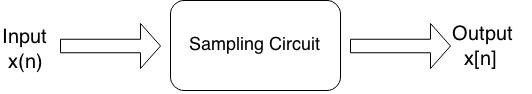
\includegraphics[width=0.5\textwidth]{block_1_.jpg}
\caption{\label{fig:}Block Diagram of a Sampling System.}
\end{figure}



One of the best examples of application of  sampling could be that of an Analog to Digital Converter (ADC). An ADC continuously take samples of the incoming data and gives an output as a sequence of discrete signals.  

The audio CDs that we play on our music systems are recorded by continuous sampling of the incoming audio signal (music) and are written on to the CD as a sequence of Digital Data sequence.



\begin{figure}[h]
 
\begin{subfigure}{0.5\textwidth}
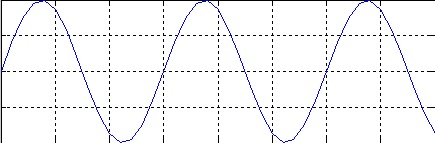
\includegraphics[width=0.9\linewidth, height=4cm]{continuous.jpg} 
\caption{Continuous Sine Wave}
\label{fig:subim1}
\end{subfigure}
\begin{subfigure}{0.5\textwidth}
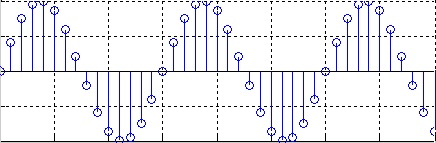
\includegraphics[width=0.9\linewidth, height=4cm]{discrete.jpg}
\caption{Discrete Sine Wave}
\label{fig:subim2}
\end{subfigure}
 
\caption{Sampling of a Continuous Sine Wave}
\label{fig:image2}
\end{figure}


\subsection{Sampling Theorem}
Also known as "Shannon-Whittaker-Nyquist theorem on Sampling".

When a signal is sampled, there is a possibility to lose information. During the sampling process, a lot of unwanted information maybe clubbed with the actual useful data.There is a need to filter out the unwanted part or the 'imposters' created by sampling.

Considerations for a given signal x(t):
\begin{enumerate}
\item The signal has a Fourier Transform.
\item The Fourier Transform is non-zero up to a maximum finite frequency $'f_m'$.
\end{enumerate}

The sampled signal is sampled at a frequency $'f_s'$.

The Sampling Theorem can be stated as:

A band-limited signal, band-limited to a maximum frequency $f_m$ can be perfectly reconstructed from it's samples taken at a rate $f_s=\frac{1}{T_s}$, such that $f_s>2f_m$ .

\subsection{Proof}


Sampling is a linear process.

Net consequence of a sampling spectrum is given by the sum of contributions by individual spectral pieces.

Consider a signal x(t), with Fourier Transform X(f).

The signal will be sampled at a frequency at a frequency $f_s$.

The Nyquist sampling theorem states that for the complete reconstruction of a signal, the sampling frequency $f_s>2f_m$.

If $f_s<2f_m$, the 'imposters' created by sampling will cloud with the original signal. Thus, resulting in loss of data. 

$f_s>2f_m$ implies $f_s-f_m>f_m$.

The imposter frequency varies from $f_s$ to $f_s-f_m$.

The Nyquist criteria ensure that since $f_s-f_m>f_m$, the imposter frequency does not mic with the actual data.

Thus, reconstructing the entire signal is basically filtering out all the 'imposters' created and only obtain the original signal.

\paragraph{}
The process of sampling will be further discussed in the next session.







\section{Lecture 7: Reconstructor: Ideal and practical}


\subsection{Introduction}
In the previous lecture, we saw that a band-limited signal can be perfectly reconstructed from its samples, if it has been sampled at a frequency greater than twice the maximum frequency of the original signal $f_{m}$. In this lecture we will see what the procedure for reconstruction is by analysing in the frequency domain. 


\subsection{Frequency response for Ideal filter for reconstruction}
It was shown that sampling creates multiple copies of the original spectrum shifted by integer multiples of the sampling frequency $f_{s}$. In order to fully reconstruct the original signal, we need a system which retains the original spectrum and cuts-off the copies as shown in Fig.\ref{copies}. 
\begin{figure}[h] 
        \centering
        
                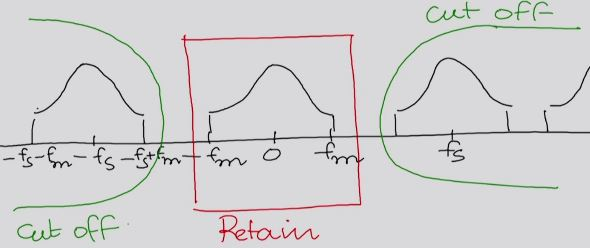
\includegraphics[width=0.8\textwidth]{aliasing.JPG}
                \caption{Principle of reconstruction}
                \label{copies}
        
\end{figure}

We can achieve this by passing the sampled signal to a LSI system with a frequency response $H(f)$ as shown in Fig.\ref{freq_response}. The filter needs to leave the signal unchanged in the frequency range $-f_{m} - \delta$ to $f_{m} + \delta$ and cut off the rest of the frequencies. 
\begin{figure}[h] 
        \centering
        
                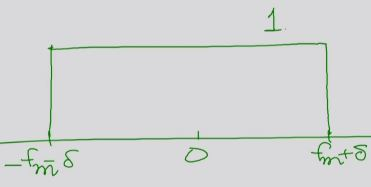
\includegraphics[width=0.8\textwidth]{freq_response.JPG}
                \caption{Desired frequency response of filter}
                \label{freq_response}
        
\end{figure}
In order to ensure that the copies are completely outside this window, we require $f_{m} + \delta < f_{s} - f_{m}$. This is because from Fig.\ref{copies}, it can be seen that there is a margin between $f_{m}$ and $f_{s} - f_{m}$. As long as the edge of the window falls inside this margin, we are good to go. 

But why do we require this margin? Why do we need to sample at \textit{greater} than twice $f_{m}$? This is because it would create a problem if our signal had a pure sinusoid exactly at $f_{m}$ i.e a \textit{tonal} component. A pure sinusoid of frequency $f_{m}$ in the time domain (a tonal component at $f_{m}$) would imply an impulse at $f = f_{m}$ in the frequency domain. Let us consider such a tonal component and see what happens if we were to sample it exactly at twice its frequency, $f_{s} = 2f_{m}$. This means that we have two samples in every period. In the unlucky event that we sampled at the zero-crossing of the sinusoid, all our samples will simply have a value $0$ as shown in green in Fig.\ref{exact_2}. 
\begin{figure}[h] 
        \centering
        
                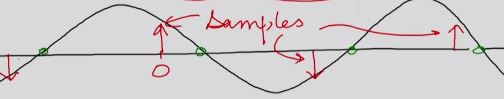
\includegraphics[width=0.8\textwidth]{exact_2.JPG}
                \caption{Sampling at exactly twice $f_{m}$ may yield all samples to be zero}
                \label{exact_2}
        
\end{figure}

Additionally, the filter should have a cut-off frequency beyond $f_{m}$ as we want to retain the tonal component at $f_{m}$. Hence the margin is necessary. 

\subsection{Impulse response of ideal filter for reconstruction}
To find this, we have to compute the inverse Fourier transform of the filter shown in Fig.\ref{freq_response}. 
\begin{equation} \label{deriv}
\begin{split}
h(t)   & = \int_{-\infty}^{\infty} H(f)e^{j2\pi ft}df \\
       & = \int_{-f_{m}-\delta}^{f_{m}+\delta} 1. e^{j2\pi ft}df \\
       & = \frac{e^{j2\pi ft}}{j2\pi t} \rvert_{-f_{m}-\delta}^{f_{m}+\delta} \\
       & = \frac{e^{j2\pi ft}}{j2\pi t} \rvert_{-f_{c}}^{f_{c}}  \mbox{ where } f_{c} = f_{m} + \delta \\
       & = \frac{e^{j2\pi f_{c}t} - e^{-j2\pi f_{c}t}}{j2\pi t} \\
       & = \frac{2j\sin (2\pi f_{c}t)}{j2\pi t} 
\end{split}
\end{equation}

The impulse response is basically a \textit{sinc} function. It goes to zero at all integer values of the argument, i.e when $2f_{c}t$ is an integer. 

\subsection{Problems with the ideal reconstructor}
\subsubsection{Stability}
Is the system given by the impulse response $h(t)$ as in \eqref{deriv} a stable system? It can be proven that it is not. For stability we require,
\begin{equation} \label{unstable}
\int_{-\infty}^{\infty} |h(t)|dt < \infty
\end{equation}
\textbf{Challenge} : Show that the above inequality does not hold. In other words, show that the absolute integral of $h(t)$ diverges thereby rendering the system unstable. \\
\textbf{Hint} : Split the integral into pieces. Find some quantity which is smaller than these pieces. Then show that the sum of the smaller quantity diverges meaning that the sum of the actual pieces will definitely diverge. $h(t)$ looks as in Fig.\ref{sinc}.
\begin{figure}[h] 
        \centering
        
                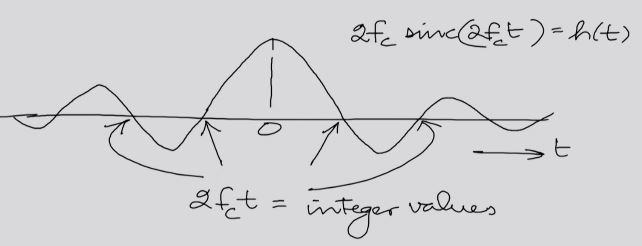
\includegraphics[width=0.8\textwidth]{sinc.JPG}
                \caption{Impulse response $h(t)$}
                \label{sinc}
        
\end{figure}

In $|h(t)|$, the negative parts get reflected about the $x$-axis and become positive. \\
Step 1 : Take each of the segments or lobes. \\
Step 2 : Lower bound each of these areas. \\
Step 3 : Show that the sum of these lower-bound areas is itself divergent.\\

\textbf{Note} :  This kind of a frequency response is called as a \textit{brick wall} response because of its structure. Brick-wall responses are always unstable systems. However although this system is unstable, its impulse response has a Fourier transform. In general this need not be the case. It means that if we give this system an input of a sinusoid, we are guaranteed a sinusoid output but there may very well be some bounded inputs whose outputs turn out to be unbounded. Hence while trying to reconstruct a bounded sampled signal, we may end up with an unbounded output if we were to use this filter. \\

What can we do about it? Recall the margin in the frequency response that we asked for earlier. We can make use of this to create a filter which is not brick wall-like and stable. Consider the frequency response of sampled signal (only with frequency values shown) as in Fig. \ref{margin}. 
\begin{figure}[h] 
        \centering
        
                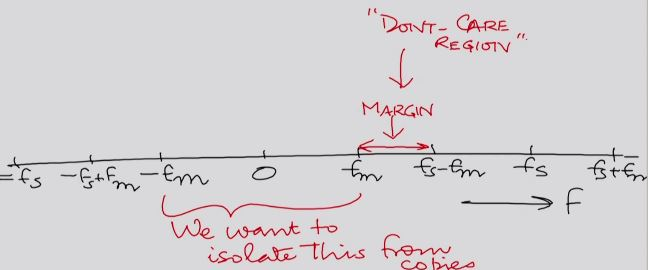
\includegraphics[width=0.8\textwidth]{margin.JPG}
                \caption{Making use of the margin or the \textit{don't care region} to construct a stable filter}
                \label{margin}
        
\end{figure}
As there is no frequency present in the margin, we do not really care what the filter does to those frequencies, or in other words, the frequency response at those frequencies is immaterial. Using this fact, we can use a filter which is not brickwall-like as in Fig.\ref{not_brick}, for example. 
\begin{figure}[h]
        \centering
        
                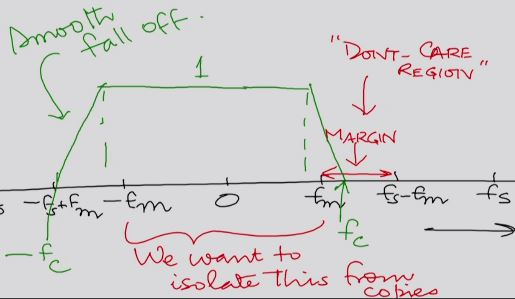
\includegraphics[width=0.8\textwidth]{not_brick.JPG}
                \caption{Example of a filter which is not brickwall-like, but still serves our purpose}
                \label{not_brick}
        
\end{figure}
This kind of a filter has a frequency response which is \textit{continuous}, unlike the brickwall filter (which had a discontinuity at $f = f_{c}$). So the margin has allowed us to make a stable filter. How large can the margin be? It is governed by the difference between $f_{s}$ and $2f_{m}$. 
\newpage
\subsubsection{Realisability}
Look at both the brickwall filter and the modified stable filter which was continuous. Both have a flat region between $-f_{m}$ and $f_{m}$. It is impossible to realise this practically. The flat region in the frequency response brings in \textit{irrationality} into the response and irrational systems require infinite resources to realise. 

We can make things more practical. Let us try to make a filter which varies \textit{slowly} in the previously flat region. Beyond this region it can be allowed to vary fast (Fig. \ref{vary}).
\begin{figure}[h] 
        \centering
        
                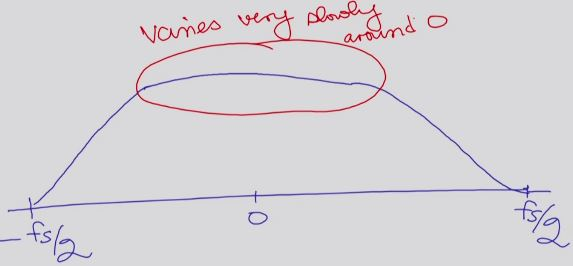
\includegraphics[width=0.8\textwidth]{vary.JPG}
                \caption{A filter which is practically realisable}
                \label{vary}
        
\end{figure}


\section{Lecture 8: An example of reconstructor }

\subsection{Introduction}
In the previous lecture, we discussed about a practical recontructor and its various properties. In this lecture, we discuss about a simple RC circuit which behaves as a reconstructor. We also discuss the magnitude response of an RC circuit, plot its graph and the limitations of ideal sampling.  

\subsection{An Example: RC circuit}
In this lecture, the concept of sampling and reconstruction is made practical and physically realizable. The simple RC combination is used as a reconstructor. The following figure depicts an RC circuit:


\begin{figure}[ht]
\centering
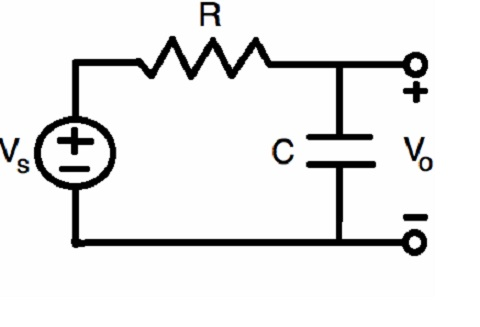
\includegraphics[width=0.3\textwidth]{circuit_RC_1.jpg}
\caption{RC circuit.}
\end{figure}

\subsubsection{Graphical approach to calculate rate of change of frequency response}

\noindent The frequency response of the given circuit is H($\Omega$).\\
Let $\Omega$ be the angular frequency.\\
Let $\tau$ = RC.\\
Then,\\ 
H($\Omega$)=$\frac{1}{1+jRC\Omega}$\\
\\
\large Magnitude of frequency response of the RC circuit is  \\

|H($\Omega$)|= $[\frac{1}{(1+(\tau \Omega)^2)}]^{1/2}$\\

\noindent Therefore the graph of the magnitude response of the RC circuit is as shown below:\\

\begin{figure}[ht]
\centering
\includegraphics[width=0.3\textwidth]{graph_1_module_3.jpg}
\caption{Magnitude response of RC circuit}
\end{figure}

\noindent From the graph it is clear that the rate of magnitude change is less near 0, then increases for some time and then the rate of magnitude change again reduces and tends to 0. 

\subsubsection{Analytic approach to calculate rate of change of frequency response}

Now we try to algebraically obtain the rate of change of magnitudes at various instants.

Taking derivative of H($\Omega$),\\
$\frac{d}{d\Omega}$|H($\Omega$)|=-$\frac{1}{2}$[$1+(\Omega \tau)^2$]$^{-3/2}$. $\frac{d}{d\Omega}[1+(\tau \Omega)^2]$
\\      
\vspace*{5mm}
=
$\frac{-\tau^2\Omega}{[1+(\tau\Omega)^2]^{3/2}}$

\noindent
Case 1:\\
Now from the equation we can see that as \\ $\Omega \rightarrow$ 0,\\
$\frac{d}{d\Omega}|H(\Omega)|$ $\rightarrow$ 0.


\vspace*{0.3 cm} 
\noindent
Case 2:\\
As $\Omega \rightarrow \infty$,\\
$\frac{d}{d\Omega}H(\Omega) \approx$ $\frac{\Omega}{\Omega^3} \approx $ $\frac{1}{\Omega^2}$

\vspace*{3 mm}
\noindent
Hence, 
	$\frac{d}{d\Omega}H(\Omega) \rightarrow 0$
\\ 
\vspace*{0.5 cm}

Hence the rate of frequency response is very less near 0 and also when the values are very large, as indicated by the graph.

\subsection{Properties of a realizable reconstructor}

RC circuit is a simple and effective reconstruct.
A stable and physically realizable reconstructor must NOT have:\\
1. A completely flat region.\\
2. A region of brickwall.\\
3. Completely zero magnitude region.\\

For a perfect reconstructor the response must become 0 after a certain interval, effectively after $f_s$/2. This is not possible for a RC circuit as it does have a non zero response after $f_s$/2.
As there are no completely flat surfaces the following errors occur:\\
1. As the frequency response has no flat region, the reconstructed signal will have slight distortions.\\
2. As the reconstructor does not have zero response, the carbon copies also have an effect in the reconstructed signal.\\

To reduce these problems of ideal sampling, non-ideal sampling is used. The next session discusses about these practical non-ideal sampling.


\section{Lecture 9: Nonideal Sampling with Pulses}


%%%%%%%%%%%%%%%%%%%%%%%%%%%%%%%%%%%%%%%%%%%%%%%%%%%%%%%%%%

\subsection{Introduction}
We are, in the current string of lectures, trying to make sense of the more practical aspects of sampling and reconstruction. We have seen so far that an RC circuit can be considered a very crude reconstructor, for a reasonable amount of scenarios. There are two conditions which we saw which must be satisfied in order for the RC circuit to work as reconstructor:
\begin{enumerate}
\item The signal should fall within the flat zone of the response of RC circuit.
\item We need to choose/modify our sampling process such that as $\Omega\rightarrow0$, the nonzero fall-off of the signal doesn't allow too much from the carbon copies of the Fourier transform of the signal to come into output.
\end{enumerate}
We will try to look how to go about satisfying the second condition:

\subsection{The Pulse Train}
We can satisfy the above condition by using nonideal sampling. So we will try to give a proof for a more generalized version of Shannon theorem which we have already seen. We will \textbf{not} be sampling with an impulse train but with a pulse train, as shown.\\
\begin{figure}[ht]
\centering
\includegraphics[width=0.7\textwidth]{fig1.png}
\caption{The Pulse Train with period $T_{s}$}
\end{figure}
Let's call this pulse train '$p(t)$' and let's try to find it's Fourier series expansion. We will use complex Fourier series, to write
\begin{align*}
C_{k}&=\frac{1}{T_{s}}\int\limits_{0}^{T_{s}} p(t) e^{-j\frac{2\pi}{T_{s}}kt}dt
\end{align*}
Where $C_{k}$ is the coefficient of the $k^{th}$ term in the Fourier series expansion, $T_{s}$ is the sampling period, and $j=\sqrt{-1}$.So we can write that expression (for nonzero $k$) as
\begin{align*}
C_{k}&=\frac{1}{T_{s}}\int\limits_{0}^{T_{s}} p(t) e^{-j\frac{2\pi}{T_{s}}kt}dt\\
         &=\frac{1}{T_{s}}\int\limits_{0}^{\Delta} e^{-j\frac{2\pi}{T_{s}}kt}dt\quad\text{as }p(t) \text{is nonzero, equal to one only in that region}\\
         &=\frac{1}{T_{s}}\left(\frac{e^{-j\frac{2\pi}{T_{s}}kt}}{-j\frac{2\pi}{T_{s}}k}\right)_{0}^{\Delta}\\
         &=\frac{e^{-j\frac{2\pi}{T_{s}}k\Delta}-1}{T_{s}\left(-j\frac{2\pi}{T_{s}}\right)k}\\
         &=\frac{1-e^{-j\frac{2\pi}{T_{s}}k\Delta}}{j2\pi k}\\
\end{align*}
We can simplify this as
\begin{align*}
C_{k}&=e^{-j\frac{2\pi}{T_{s}}k\frac{\Delta}{2}}\cdot \frac{\cancel{2j}\sin(\frac{\cancel{2}\pi}{T_{s}}k\frac{\Delta}{\cancel{2}})}{\cancel{2j}\pi k\frac{\Delta}{T_{s}}}\cdot\frac{\Delta}{T_{s}}\\
&=\frac{\Delta}{T_{s}}e^{-j\frac{2\pi}{T_{s}}k\frac{\Delta}{2}}\cdot\frac{\sin(\frac{\pi k \Delta}{T_{s}})}{\frac{\pi k \Delta}{T_{s}}}\\
&=\frac{\Delta}{T_{s}}e^{-j\frac{2\pi}{T_{s}}k\frac{\Delta}{2}}\cdot \text{sinc}\left(\frac{k\Delta}{T_{s}}\right)
\end{align*}
Where sinc function is given by
\begin{equation}
\text{sinc}(r)=\frac{\sin(\pi r)}{\pi r}\nonumber
\end{equation}
We can also scale these pulses so as to have unit area, by multiplying by $\frac{1}{\Delta}$, and it would just cancel out the delta in our expression, so we'd have 
\begin{equation}
C_{k}=\frac{1}{T_{s}}e^{-j\frac{2\pi}{T_{s}}k\frac{\Delta}{2}}\cdot \text{sinc}\left(\frac{k\Delta}{T_{s}}\right)\nonumber
\end{equation}
When $k=0$, we can show that $C_{0}$ is the limit of this expression as $k\rightarrow0$. We can also compute $C_{0}$ independently.\\
Let us plot the sinc function and see how it looks like:\\
\begin{figure}[htb]
\centering
\includegraphics[width=0.3\textwidth]{fig2.png}
\caption{The 'sinc' function.}
\end{figure}
In ideal sampling, we had $\frac{\Delta}{T_{s}}$ very small, tending to zero. In that case we had all our samples taken very closely, around zero. Applying $\Delta\rightarrow0$ to the expression of $C_{k}$ (scaled), we have $C_{k}\approx\frac{1}{T_{s}}$ .i.e. all the $C_{k}$'s are same. However, if $\Delta\ne0$, we have the expression for $C_{k}$ as stated earlier, involving sinc function. We can write it as 
\begin{equation}
C_{k}=\gamma_0\text{sinc}\left(\frac{k\Delta}{T_{s}}\right)\nonumber
\end{equation}
Here $\gamma_0$ is a constant. Let's look at the Fourier series representation of $p(t)$:
\begin{figure}[htb]
\centering
\includegraphics[width=0.3\textwidth]{fig3.png}
\caption{The sampled version of sinc($r$). $r$ is on the x-axis. Some of the $C_{i}$'s are labeled.}
\end{figure}
Note that the distance between two consecutive samples is $\frac{\Delta}{T_{s}}$. We can see that as $\Delta\rightarrow0$, we will have all our samples around zero. If $\frac{\Delta}{T_{s}}$ is quite large, after $C_{0}$, the second sample itself will be not from the main lobe. However, if we choose $\frac{\Delta}{T_{s}}$ to not be too large yet not too small, we would have first few samples from main lobe, and we can observe that they will be of decreasing magnitude.
\subsection{Sampling with the Pulse Train}
We already know that the Fourier series expansion of $p(t)$ is $\sum\limits_{k\in\mathbb{Z}}C_{k}e^{j\frac{2\pi}{T_{s}}kt}$, so multiplying it with $x(t)$, we'd have 
\begin{equation}
x(t)p(t)=\sum\limits_{k\in\mathbb{Z}}C_{k}x(t)e^{j\frac{2\pi}{T_{s}}kt}\nonumber
\end{equation}
Now let's take the Fourier transform of $x(t)p(t)$ which we have, assuming it exists. Note that, as Fourier transform is a linear transform, we can compute the Fourier transform of one term from the summation which we have, and add all such Fourier transforms. So we will compute Fourier transform of $x(t)e^{j\frac{2\pi}{T_{s}}kt}$.
\begin{align*}
\text{Fourier transform of }x(t)e^{j\frac{2\pi}{T_{s}}kt}&=\int\limits_{-\infty}^{+\infty}x(t)e^{j\frac{2\pi}{T_{s}}kt}e^{-j\Omega t}dt\\
&=\int\limits_{-\infty}^{+\infty}x(t)e^{-j\left(\Omega-\frac{2\pi}{T_{s}}k\right)}dt\\
\end{align*}
Suppose we have Fourier transform of $x(t)$ as $X(\Omega)$, then the Fourier transform of $x(t)e^{j\frac{2\pi}{T_{s}}kt}$ will be $X\left(\Omega-\frac{2\pi}{T_{s}}k\right)$, from the above equation. i.e. it is the Fourier transform of $x(t)$ namely $X(\Omega)$ shifted by $\frac{2\pi}{T_{s}}k$ forward. So we have 
\begin{align*}
&\text{Fourier transform of }x(t)e^{j\frac{2\pi}{T_{s}}kt}=X\left(\Omega-\frac{2\pi}{T_{s}}k\right)\\
\therefore\quad &\text{Fourier transform of }C_{k}x(t)e^{j\frac{2\pi}{T_{s}}kt}=C_{k}X\left(\Omega-\frac{2\pi}{T_{s}}k\right)\\
\therefore \quad&\text{Fourier transform of }\sum\limits_{k\in\mathbb{Z}}C_{k}x(t)e^{j\frac{2\pi}{T_{s}}kt}=\sum\limits_{k\in\mathbb{Z}}C_{k}X\left(\Omega-\frac{2\pi}{T_{s}}k\right)\\
\end{align*}
We can list down the procedure of finding the Fourier transform of $x(t)p(t)$ as follows:
\begin{enumerate}
\item Shift $X(\Omega)$ by $\frac{2\pi}{T_{s}k}$ forward, $\forall k\in\mathbb{Z}$.
\item Multiply this shifetd version of $X(\Omega)$ by $C_{k}$.
\item Add up all these shifted versions.
\end{enumerate}
\subsection{Graphical Representation of the Fourier Transform of the Sampled Signal}
We'll see how all of this looks graphically: Consider $x(t)$ to be bandlimited signal, as shown in the following image (magnitude of $X(\Omega)$ is shown in the image, and phase is considered to be zero for this signal everywhere:\\

\begin{figure}[htb]
\centering
\includegraphics[width=0.35\textwidth]{fig4.png}
\caption{$X(\Omega)$}
\end{figure}

Note that this Fourier representation corresponds to a real and even signal $x(t)$.\\
We will first sample this signal 'disobeying' the Nyquist principle, i.e. by keeping $\frac{1}{T_{s}}\ngeq2\frac{\Omega_m}{2\pi}$. The first few $C_{}k$ values are seen in the following image:\\

\begin{figure}[htb]
\centering
\includegraphics[width=0.3\textwidth]{fig3.png}
\end{figure}

Following the procedure given in the previous section, we obtain following spectrum for the sampled $x(t)$:\\

\begin{figure}[htb]
\centering
\includegraphics[width=0.7\textwidth]{fig5.png}
\caption{Fourier transform when we disobey Nyquist principle: shows overlaps.}
\end{figure}

One feature we can clearly see in this graph is that carbon copies of the original spectrum are overlapping: which we had already seen when we had sampled a similar signal with impulse train instead of pulse train (ideal sampling). However, there's one more remarkable thing we can see here: As the first few $C_k$'s are decreasing in magnitude, we observe that the 'strength' of the carbon copies is reducing, at least for first few $k$'s. So the carbon copies still overlap, but their strength is lower, or, the magnitude of overlap is less now, the region in which such overlap is occuring is closer to the original spectrum, if compared with the Fourier transform of the same signal, sampled using impulse train.\\
Now we will see what happens if we sample this signal 'obeying;' the Nyquist principle, i.e. $\frac{1}{T_{s}}\gg2\frac{\Omega_m}{2\pi}$. This time we obtain the spectrum of the sampled signal as following:\\

\begin{figure}[htb]
\centering
\includegraphics[width=0.7\textwidth]{fig6.png}
\caption{Fourier transform when we obey Nyquist principle: no overlap is seen.}
\end{figure}

Here, no overlap is seen between the original spectrum and any of its carbon copies, similar to when we had sampled using impulse train. But we can still see the magnitude of the first few carbon copies decreasing.\\
When reconstructing the signal back in this case, still need our spectrum to lie in the 'flat' region of the spectrum of the reconstructor (a simple practical example of which,  we have seen, is a simple $RC$- circuit). So pracically$\Omega_s$ needs to be much higher htan $\Omega_m$There is one more advantage of using pulse train instead of impulse train to sample a signal: for a practical reconstructor, it's spectrum desn't become zero directly after the flat region- it gradually tends towrd zero. So while reconstructing the signal, the higher-frequency carbon copies of the original spectrum aren't completely eliminated. Since we anyway have reducing magnitude for the carbon copies in the spectrum of the signal sampled using pulse train, we have lesser contribution from these high-frequency components than the reconstructed signal from the ideal sapmle of the signal.\\
We shall also give a name to these carbon copies: we will call them 'aliases' and this process 'aliasing' henceforth. Alias refers to the act of assuming a different identity. Here, original spectrum 'pretends' to be a spectrum around some $\Omega_s$. If these aliases interfere with each otherm it only causes confusion, Nyquist theorem essentially tells us htat we don't want aliasing.

\section{Lecture 10: Nyquist Sampling Theorem: Proof and Application}

\subsection{Introduction}
Till now, we have talked about ``ideal'' sampling, where the sampling was done using impulses. We have also done sampling using \emph{pulses}, instead of impulses. In this lecture, we will look at a ``generalized version'' of the sampling, which is called ``amplitude modulation''.  We will also prove a more general form of the Nyquist-Shannon sampling theorem.


%signals, that is, you only ``read'' and ``store'' the value of the signal at certain points. We saw the problems associated with sampling, mainly the fact that given just the sampled signal, it is not possible to reconstruct the original signal, because there are many possible signals which would have given the \emph{same} samples, i.e. they would have taken on the same values as this signal at the points where we are sampling. The natural question to ask, then, is what ``extra information'' do we need in order to reconstruct the original signal from this sample? To do that, we first have to know what these ``other signals'' look like.

\subsection{General form of the Nyquist-Shannon Sampling Theorem}
We have looked at sampling in some detail in the previous lectures. We will now generalize this idea of sampling. Earlier, for ``ideal'' we multiplied the signal with a train of impulses placed at regular intervals. Now, what we are going to do is that we will multiply the signal with any ``carrier signal'' $p(t)$, and the only requirement that we are going to make of $p(t)$ is that it be periodic with period $T_s$. This signal, as a result of this periodicity, will have a complex Fourier series expansion:
\[ p(t) = \sum\limits_{k=-\infty}^{+\infty} c_k e^{\imath\frac{2\pi}{T_s}kt}\]
Let the signal to be ``sampled'' be $x(t)$, and I put the word ``sampled'' in quotes because what we're doing here can't really be called sampling. We need $x(t)$ to have a Fourier transform $X(\Omega)$. Now we ``sample'' this $x(t)$ using $p(t)$, (which is to say we multiply the two) to obtain $x(t) p(t)$. The Fourier Transform of this $x(t) p(t)$ is $X_s(\Omega)$ (say).

\begin{align*}
X_s(\Omega)&=\mathcal{F}\left(x(t) p(t)\right)\\
&=\mathcal{F}\left(x(t) \sum\limits_{k=-\infty}^{+\infty} c_k e^{\imath\frac{2\pi}{T_s}kt}\right)\\
&=\sum\limits_{k=-\infty}^{+\infty}c_k\mathcal{F}\left(x(t) e^{\imath\frac{2\pi}{T_s}kt}\right) \tag{$k$ is independent of $t$}\\
&=\sum\limits_{k=-\infty}^{+\infty}c_k X\left(\Omega-\frac{2\pi}{T_s}k\right)
\end{align*}
As an example, let's see what happens with $p(t)=A_c\cos\left(\frac{2\pi}{T_s}t\right)$, which can also be written as
\[p(t)=\frac{A_c}{2}\left(e^{\imath\frac{2\pi}{T_s}t} + e^{-\imath\frac{2\pi}{T_s}t}\right)\]
Thus, we have
\[X_s(\Omega)=\frac{A_c}{2}\left\{ X\left(\Omega-\frac{2\pi}{T_s}\right)+ X\left(\Omega+\frac{2\pi}{T_s}\right)\right\}\]
And this is \emph{precisely} what is known as \emph{amplitude modulation}. This $p(t)=A_c\cos\left(\frac{2\pi}{T_s}t\right)$ is called the \emph{carrier wave}, and $x(t)$ is said to have been modulated with this carrier. This modulation has the effect of creating two copies of the signal and shifting each one of them forward and backward respectively, in the frequency domain. And if the carrier frequency is large enough, these two copies don't ``overlap'' (or ``mix'') with each other.

Therefore, in applying the Nyquist theorem, we have essentially carried out amplitude modulation (instead of sampling, as is usually done).

It's worthwhile to note that we need not have used a pure sinusoid to modulate the signal. In fact, as we have stated before, we could have used any periodic signal! This is important when we start designing and building systems (say electronic circuits), as it is difficult to build systems like multipliers and sinusoid generators, which are necessary for amplitude modulation with pure sinusoids. %And the above example gives us an idea as to how we can go about doing it.

Instead, a much simpler way to do modulation is to just use a train of pulses. It is easy to see that modulation using a pulse train (which is essentially just multiplication with said pulse train) is equivalent to just switching the signal on and off (and scaling it) at regular intervals! And building such a circuit would be much easier.

So we choose $p(t)$ to be a pulse train of period $T_s$, having pulse width $\Delta$ and height $\frac{1}{\Delta}$. Doing this, we obtain a spectrum as shown in Figure~\ref{fig:pulsemodspectrum}. As we can see, the first two carbon copies (the ones corresponding to $c_1$ and $c_{-1}$) are the ones we want, as they are the ones that appear in the usual amplitude modulation with a sinusoid.

We want to retain only the ``carbon copies'' corresponding to  $c_1$ and $c_{-1}$ and get rid of the $c_0$, $c_2$ and $c_{-2}$, $c_3$ and $c_{-3}$\ldots terms. To do that, we use a \emph{band-pass filter} as shown in Figure~\ref{fig:bandpassspectrum}.

A band pass filter, as the name suggests, only allows a certain \emph{range} of frequencies to go through, and \emph{blocks} all other frequencies. An ideal band-pass filter has a frequency response of $G$ in the \emph{passband} (the range of frequencies to be passed) and $0$ in the \emph{stop-band} (everywhere except the passband). The frequency response of a more \emph{practical} band pass filter is shown in Figure~\ref{fig:practpassband}. The frequencies at the boundary of the passband and stop band form the transition band. In this region, the impulse response undergoes a smooth transition. In a practical bandpass filter, you can't make the frequency response in the passband constant, you can't make the frequency response in the stop band exactly zero, and you can't make the transition band infinitesimally small.

Therefore, this filter \emph{will} pass parts of the other copies of the original spectrum, but these will be \emph{attenuated} (scaled down). Broadly speaking, this is how amplitude modulation is done, in practice.


\section{Lecture 11: Sample and Hold}

\subsection{Introduction}
In the last session we have seen that sampling is actually multiplying an input signal with a periodic waveform. Sampling is about representing the signal more efficiently than the raw form. 
In this discussion we discuss the problem of reconstruction of the signal if we put in place systems to interpolate the signal from the sampled signal.
%about what we want to do with the sampled signal, i.e. whether we want to hold on to the sampled signal or just let it go. 

\subsection{Interpolation}
Interpolate means to complete the waveform in between the samples. Interpolation is a method of constructing new data points within the range of a discrete set of known data points.

\subsubsection{Graphical Explanation}

Let us consider a function as shown in fig. 1 and sample it with a time period of $T_{s}$.

\begin{figure}[ht]
\centering
\includegraphics[width=0.6\textwidth]{M3L11-fig1.jpg}
\caption{A sampled function}
\end{figure}

There are various ways in which we can interpolate the given samples\\


\noindent Method 1: Sample and Hold\\
\noindent In figure 2, the red lines form the interpolated signal using the Sample and Hold method.

\begin{figure}[ht]
\centering
\includegraphics[width=0.6\textwidth]{M3L11-fig2.jpg}
\caption{Sample and Hold}
\end{figure}


\noindent Method 2: Linear interpolation\\
In this method the sampled points are connected by straight lines. Refer to figure 3 for linear interpolation.
In Figure 3, the green lines form the linearly interpolated signal obtained by interpolating from the sampled signal.



\begin{figure}[ht]
\centering
\includegraphics[width=0.6\textwidth]{M3L11-Fig3.jpg}
\caption{Linear interpolation}
\end{figure}


Other kinds of interpolations are also possible. But in this discussion we shall focus on sample and hold.

\subsubsection{Systematical explanation}

Systematically the sample and hold can be understood as follows:

\begin{figure}[ht]
\centering
\includegraphics[width=0.7\textwidth]{M3L11-fig4.jpg}
\caption{Systematical representation of sample and hold}
\end{figure}

The impulse response of the linear shift invariant system in the above figure is a pulse as shown in fig 5.

\begin{figure}[ht]
\centering
\includegraphics[width=0.5\textwidth]{M3L11-Fig5.jpg}
\caption{Impulse response of linear shift invariant system.
}\end{figure}

\subsection{Frequency domain analysis}
The LSI system which follows the ideal sampler is called the Hold system. This is because, the effect of this system on a sampled signal is that of retaining the sampled value till the next sample is reached. Note that since the Hold system impulse response has a finite value in a finite interval, it is absolutely integrable and hence it is a stable system.
%The hold system can be stated to be stable as the impulse response is absolutely integrable. 
\\
Now, the frequency response of the Hold system is:

\begin{align*}
H(\Omega) &=\int\limits_{-\infty}^{\infty}\mathrm{h(t)}{e}^{-jt\Omega}\,\mathrm{d}\\
&=\int\limits_{0}^{T_{s}}\mathrm{e}^{-jt\Omega}\,\mathrm{d}t\\
&=\left.\frac{e^{-jt\Omega}}{-j\Omega}\right|_0^{T_{s}}\\
&=\frac{1-e ^{-j\Omega T_s}}{j \Omega}\\
&=\frac{e^\frac{-j \Omega T_s}{2} \left(e^{\frac{j \Omega T_s}{2}} - e^{\frac{-j \Omega T_s}{2}}\right)}{j \Omega}\\
&=\frac{T_s}{2} e^{\frac{-j \Omega T_s}{2}} \frac{2j \sin{\frac{\Omega T_s}{2}}}{j \frac{\Omega T_s}{2}}\\
&=T_s e^\frac{-j \Omega T_s}{2}\frac{2j}{2j} \frac{\sin{\frac{\Omega T_s}{2}}}{\frac{\Omega T_s}{2}}\\
&=T_s e^{\frac{-j \Omega T_s}{2}} \frac{\sin{\Omega T_s/2}}{\Omega T_s/2}
\end{align*}

%$$= \int\limits_{-\infty}^{\infty}\mathrm{h(t)}{e}^{-jt\Omega}\,\mathrm{d}t$$

%$$= \int\limits_{0}^{T_{s}}\mathrm{e}^{-jt\Omega}\,\mathrm{d}t$$
%$$= \left.\frac{e^{-jt\Omega}}{-j\Omega}\right|_0^{T_{s}}=\frac{1-e ^{-j\Omega T_s}}{j \Omega}$$


%$$= \frac{e^\frac{-j \Omega T_s}{2} \left(e^{\frac{j \Omega T_s}{2}} - e^{\frac{-j \Omega T_s}{2}}\right)}{j \Omega}$$
%$$=\frac{T_s}{2} e^{\frac{-j \Omega T_s}{2}} \frac{2j sin{\frac{\Omega T_s}{2}}}{j \frac{\Omega T_s}{2}}$$
%$$=T_s e^\frac{-j \Omega T_s}{2}\frac{2j}{2j} \frac{sin{\frac{\Omega T_s}{2}}}{\frac{\Omega T_s}{2}}$$
%Frequency response
%{\Large
% = $T_s e^{\frac{-j \Omega T_s}{2}} \frac{sin{\Omega T_s/2}}{\Omega T_s/2}$
%}

\subsubsection{Frequency domain analysis}

Let $x(t)$ obey Nyquist principle. Hence band limited to $\frac{1}{2 T_s}$.
Consider such an $x(t)$ with Fourier Transform as shown in Figure 6.
%\noindent If $x(t)$ is band limited, the Fourier transform in ycles/second is as follows:

\begin{figure}[ht]
\centering
\includegraphics[width=0.9\textwidth]{M3L11-fig6.jpg}
\caption{Fourier transform of x(t)}
\end{figure}

Then, after passing the signal through the ideal sampler, the sampled signal obtained, $X_s(t)$, will have the spectrum $X_s(f)$ as shown in Figure 7.


\begin{figure}[ht]
\centering
\includegraphics[width=0.9\textwidth]{M3L11-Fig7.jpg}
\caption{Spectrum of the sampled signal: $X_{S}(f)$}
\end{figure}

Sketch of 'hold' frequency response.

$$ H(f) = T_s e^{-j \pi fT_s}\frac{sin \pi fT_s}{\pi fT_s}$$

Magnitude $\implies$

\begin{figure}[ht]
\centering
\includegraphics[width=0.9\textwidth]{M3L11-Fig8.jpg}
\caption{Hold frequency response}
\end{figure}

If we superimpose both hold frequency response and $X_s(f)$,

\begin{figure}[ht]
\centering
\includegraphics[width=1.2\textwidth]{M3L11-Fig9.jpg}
\caption{Superimposing hold freq. response on $X_{s}(f)$}
\end{figure}


In process of sampling and holding, two problems are
\begin{enumerate}
\item Aliases pass through partially
\item Original gets distorted
\end{enumerate}


Hence, equalization is needed in the original spectral band of

$-\frac{1}{2T_s} \rightarrow \frac{1}{2T_s}$

Equalization is the reciprocal of the hold frequency response given by\\
{\large
$$\frac{1}{T_s e^{-j \pi f T_s}\frac{\sin \pi fT_s}{\pi f T_s}}
\mbox{  for} -\frac{1}{2T_s} < f <  \frac{1}{2 T_s}$$
}
\newpage

Sketch of equalizer frequency response.

\begin{figure}[ht]
\centering
\includegraphics[width=0.7\textwidth]{M3L11-Fig_10.jpg}
\caption{Equalizer freq. response}
\end{figure}


Hence to reconstruct a signal after sample and hold, two things are required:
\begin{enumerate}
\item To remove the aliases
\item To equalize
\end{enumerate}

The ideal reconstructor for sample and hold has to
\begin{enumerate}
\item Equalize in signal band
\item Stopband outside sigal band
\end{enumerate}

In the next lecture, we will discuss about linear interpolation.


\section{Lecture 12: Sampling followed by Linear Interpolation}


\subsection{Introduction}
In the previous section, we have seen the working of a Sample and Hold circuit. We can now say that the Sample and hold circuit is nothing but an Ideal Sampling System followed by a Linear Shift Invariant system.

We have also seen the drawbacks of the sample and hold circuit which include:

\begin{enumerate}
\item Distortion in the original spectrum.
\item Aliases also pass through the circuit partially.
\end{enumerate}

We will now look at the procedure that will be followed by the Sample and Hold circuit.
\subsection{Linear Interpolation}
Linear Interpolation can be broadly defined as the joining of two known points by a straight line.

Thus, if we know two given points, the linear interpolant will be the straight line joining these two lines. 

\begin{figure}[h]
\centering
\includegraphics[width=0.9\linewidth, height=4cm]{LinInt.jpg}
\caption{Linear Interpolation of given points.}
\end{figure}

Above figure indicates a rough sketch of Linear Interpolation of a given set of points. 



\pagebreak

\subsection{Signal Representation of Linear Interpolation}

We now look at the effect of the Linear Interpolation on a given signal $x(t)$.

Signal $x(t)$ is passed through an ideal sampler, with sampling interval $Ts$.

It is then passed through a Linear Shift Invariant system.

\begin{figure}[h]
\centering
\includegraphics[width=0.7\linewidth, height=3cm]{M3L12-fig4.jpg}
\caption{Passing x(t) through the Sample and Hold Circuit.}
\end{figure}

The impulse response of the Linear Shift Invariance will be triangular in nature as shown below. 
We sketch the original signal $x(t)$, the ideal sampling output $xs(t)$ and the scaled and shifted impulse response of the Linear Shift Invariant System given by $x(nTs).h(t-nTs)$

\begin{figure}[h]
\centering
\includegraphics[width=0.9\linewidth, height=4cm]{graph1.jpg}
\caption{Signal Representation along with the Sampling output and the Impulse response of LSI system}
\end{figure}

The shifted and scaled impulse responses are now added linearly. As seen before, linear interpolation is the joining of two points with a straight line.

We now add the $green$ straight lines between the various time intervals. Additions of two straight lines will also be a straight line. 

The resulting addition of these straight lines will be the Linear Interpolated Signal and can be seen in $blue$ in the figure below.
\pagebreak

\begin{figure}[h]
\centering
\includegraphics[width=0.9\linewidth, height=4cm]{graph2.jpg}
\caption{Signal Representation along with the Sampling output and the Impulse response of LSI system}
\end{figure}

Idea of Linear Interpolation for a signal can be stated as the passing of an ideally sampled output through a Linear Shift Invariant system.

\subsection{Significance in frequency domain}

Convolution of a signal with itself can be seen as the multiplication of it's Fourier Transform with itself. 

The sample signal $h0(t)$ can be shifted to the time interval $-Ts/2$ to $Ts/2$.This gives us the Zero order hold. 

Convolution $h0(t)$ with itself gives us the first order hold. It can be seen in the given diagram.
\begin{figure}[h]
\centering
\includegraphics[width=0.9\linewidth, height=4cm]{graph3.jpg}
\caption{Convoluting the Zero order hold with itself}
\end{figure}
\pagebreak

\subsubsection{Mathematical representation}

Frequency Response of first order hold:
$$Ts.\exp(-jt\omega).\frac{sin(\frac{Ts}{2}\omega)}{\frac{Ts}{2}\omega}.\exp(\frac{Ts}{2}\omega)$$

Squaring the above term, we get:

$$Ts^2.(\frac{sin(\frac{Ts}{2}\omega)}{\frac{Ts}{2}\omega})^2$$

The implications will be as follows:
\begin{enumerate}
\item sinc(fTs) has a maximum value of 1.
\item We know that the function $sinc(fTs)$<1. Therefore, squaring the function will result in further reduction of magnitude.
\item The function will thus fall at a faster rate.
\end{enumerate}

We can thus conclude from above that the given operation has the following effects on the signal band:

\begin{description}
\item[Advantages] We can thus see that the side lobes are now lower. The other aliases that were formed are suppressed as compared to the Zero order hold.

\item[Disadvantage] Along with the side lobes, the major lobe too will now be suppressed to some extent. The region from $-Ts/2$ to $Ts/2$ suffers a steeper drop.  
\end{description}







\section{Lecture 13: Applications of Discrete Time Processing}


\subsection{Introduction}
In the previous lectures in Module 3, we have studied the concepts of sampling of continuous independent variable signals and reconstruction from the sampled signals. In some ways, we thus converted a continuous signal into a discrete one in the process of sampling. Now we wish to apply these concepts learnt to practical scenarios. We motivate this application below.

\subsection{Why Digital Systems over Continuous Systems?}
\subsubsection{Digital vs Discrete Signals}
We first bring out the difference between a digital system and a discrete system. A discrete signal means that the independent variable takes on discrete values rather than continuous values. This we already know. Thus sampling a continuous signal leads to a discrete signal. The result of sampling, a discrete signal, however, takes on arbitrary real values. Implementing this in practice is not possible as we can only represent fixed precision numbers in all our processing devices. Thus, we need to discretise the values taken by the sampled signal i.e. we need to discretise the dependent variable too. The result is then called a digital signal. We give an example below.

%% some image of a sampled and a quantised signal.

\subsubsection{Discrete vs Continuous Signals}
We have already talked about how discrete signals (and digital signals more so) are convenient for processing and and also that they are robust against noise. Somewhat similar is the case with digital and continuous systems. We list below some advantages of digital systems over continuous systems.

\begin{enumerate}
\item \textbf{Flexibility}\\
Digital systems are generally implemented on a digital signal processor (DSP) which, in layman's terms, basically are just computers. The jargon just makes it sound frightening. As is the case with a computer, even a DSP can be made to do a lot of diverse things without much effort. Thus, we just need to change the program and we get a new system implemented without much effort. That however, is not the case with an analog system as it is generally highly specialized and hence restrictive.
\item \textbf{Easy and Low Maintenance}\\
Generally, digital circuit components have a longer life as compared to analog components. Also, a digital system, is by construction more modular as compared to an analog one leading to easy replacement of parts when necessary.
\item \textbf{Generality}\\
Designing an analog system for any given frequency response is often challenging and even practically impossible. This however is not the case with digital systems where we can get as close to the desired response as needed with more processing and possibly more memory.
\end{enumerate}

\subsection{A Digital System}
From the above discussion, it is clear that digital systems are preferred over continuous systems practically. However, the practical world is an analog one and hence the signals there are continuous signals. To use a digital system to process a real world signal, we need to convert the signal into a digital signal, then process it using a DSP and then reconvert it back to an analog signal for it to be of any use to us. This architecture is shown in in figure 1.

\begin{figure}
 	\includegraphics[width=\textwidth]{dsp.jpg}
    \caption{Processing a Continuous Signal Using a DSP}
\end{figure}

As is seen in the figure, we need to sample the input signal (discretise the independent variable) and later quantise it (discretise the dependent variable). Sampling necessitates that the input signal be bandlimited. This is in general not an issue because most of the signals in real life are practically bandlimited given a sufficient frequency range.

\subsection{A Speech Processing System}
We now take a concrete example of a speech signal and discuss the above structure of a digital system in that context.
As we know, a speech signal is generally bandlimited to $4 kHz$. In that case, the Nyquist Sampling Theorem tells us that the signal be sampled at a sampling frequency of more than $8 kHz$. We also, however, know that a margin is better for ease of reconstruction. Thus we decide the sample the speech signal at a frequency of $10 kHz$ i.e. we record 10,000 samples per second. 


\begin{figure}[H]
    \includegraphics[width=\textwidth]{speech.jpg}
    \caption{Spectrum of a Speech Signal}
\end{figure}%
       

\begin{figure}[H]
    \includegraphics[width=\textwidth]{sampled_speech.jpg}
    \caption{Spectrum of the Sampled Speech Signal}
\end{figure}

Let the frequency spectrum of the speech signal be as shown in figure 2(a) (Note that this is not the spectrum of a real speech signal - which is a lot more complicated - but an illustrative plot) On sampling this signal at $10 kHz$, we get the spectrum shown in figure 2(b). 


\begin{figure}[H]
 	\includegraphics[width=\textwidth]{dig.jpg}
    \caption{A Digital System}
\end{figure}

We then pass these digital samples (which now are just bits) into the digital signal processor to process the signal as desired. %%% What did the DSP do? %%%.
A schematic of this discrete system is shown in figure 4. A discrete system takes as input the input samples and concurrently gives a sequence at the output. After this processing is done, we reconstruct an output signal from the samples from the DSP using a DAC as shown in figure 1.


\subsection{An Overview of a Successive Approximation ADC}
Here we present an overview of a successive approximation analog to to digital converter. A block schematic is given in figure 5. As the name suggests, we start with an approximate binary value of the input voltage and successively (iteratively) improve this approximation. We convert the current approximation of the input (a binary value) into an analog signal with the help of a voltage combiner (this is just a DAC which we look at in the next section). The output of this combiner and the input voltage are then passed to a comparator. Depending on the result of the comparator, we increase or decrease the value of the current approximation (i.e. we improve the approximation in this step). This continues till we can no longer improve the approximation because of the limited precision of the finite number of binary bits available to us.
\begin{figure}[H]
 	\includegraphics[width=\textwidth]{saadc.jpg}
    \caption{Successive Approximation ADC}
\end{figure}
\subsection{An Overview of a DAC}
Now, we describe a Digital to Analog Converter (DAC). In general, a DAC takes a $n$-bit binary number and converts it into a voltage proportional to the value of the input binary number. We consider the case of a 4-bit DAC as shown in figure 6. $V_{0}$, $V_{1}$, $V_{2}$ and $V_{3}$ are the 4 bits (We assume that the bit $1$ corresponds to a voltage of $5V$ and the bit $0$ corresponds to a voltage of $0V$.). $R_{0}$, $R_{1}$, $R_{2}$, $R_{3}$ and $R_{L}$ are resistors such that $R_{1} = 2R_{0}$, $R_{2} = 4R_{0}$ and $R_{3} = 8R_{0}$. As shown, $I_{0}$, $I_{1}$, $I_{2}$, $I_{3}$ and $I_{L}$ are currents through the resistors $R_{0}$, $R_{1}$, $R_{2}$, $R_{3}$ and $R_{L}$ respectively.
\begin{figure}
 	\includegraphics[width=\textwidth]{dac2.jpg}
    \caption{A Possible DAC}
\end{figure}




We have, by Ohm's Law,


\begin{align*}
I_{0} &= \frac{V_{net} - V_{0}}{R_{0}}\\
I_{1} &= \frac{V_{net} - V_{1}}{R_{1}}\\
I_{2} &= \frac{V_{net} - V_{2}}{R_{2}}\\
I_{3} &= \frac{V_{net} - V_{3}}{R_{3}}\\
I_{L} &= \frac{V_{net}}{R_{L}}
\end{align*}



In that case, by Kirchoff's Current Law (KCL), we have, 


\begin{equation*}
	I_{L} = I_{0} + I_{1} + I_{2} + I_{3}
\end{equation*}

Thus,

\begin{align*}
       \frac{V_{net}}{R_{L}} &= \frac{V_{net} - V_{0}}{R_{0}} + \frac{V_{net} - V_{1}}{R_{1}} + \frac{V_{net} - V_{2}}{R_{2}} + \frac{V_{net} - V_{3}}{R_{3}}\\
                             &= \frac{V_{net} - V_{0}}{R_{0}} + \frac{V_{net} - V_{1}}{2R_{0}} + \frac{V_{net} - V_{2}}{4R_{0}} + \frac{V_{net} - V_{3}}{8R_{0}}\\
\end{align*}

Rearranging,

\begin{align*}
	V_{net} (\frac{1}{R_{L}} + \frac{1}{8R_{0}} + \frac{1}{4R_{0}} + \frac{1}{2R_{0}} + \frac{1}{R_{0}}) &=
    \frac{V_{3}}{8R_{0}} + \frac{V_{2}}{4R_{0}} + \frac{V_{1}}{2R_{0}} + \frac{V_{0}}{R_{0}}
\end{align*}

If,

\begin{equation*}
	G_{L1} = (\frac{1}{R_{L}} + \frac{1}{8R_{0}} + \frac{1}{4R_{0}} + \frac{1}{2R_{0}} + \frac{1}{R_{0}})
\end{equation*}

and 

\begin{equation*}
	G_{0} = \frac{1}{R_{0}}
\end{equation*}

Here $G$ stands for conductance, the inverse of resistance. Then we have,

\begin{equation*}
	V_{net} = \frac{G_{0}}{G_{L1}}\frac{1}{8}V_{3} + \frac{G_{0}}{G_{L1}}\frac{1}{4}V_{2} + \frac{G_{0}}{G_{L1}}\frac{1}{2}V_{1} + \frac{G_{0}}{G_{L1}}V_{0}
\end{equation*}


Thus, if $V_{0}$ corresponded to the Most Significant Bit (MSB) of the input binary number and $V_{3}$ corresponded to the Least Significant Bit (LSB), then $V_{net}$ is proportional to the value of the input binary number as is seen. The proportionality constant does not matter a lot because we can always amplify a given voltage if necessary.



\subsection{Frequency Normalisation}
Before we start discussing concrete discrete (or digital) systems, we need get a few boring things out of the way. Notation and convention is one of them. We discuss here something called frequency normalisation. This basically means that we look at quantities all relative to the sampling frequency (or equivalently the sampling interval). Thus, we consider one sampling interval to be a unit length of time. The sampling frequency, which is equal to the reciprocal of the sampling interval (which is now equal to one unit of time) also is equal to unity in these normalised units. Thus, in order to avoid aliasing, according to Nyquist's theorem, the maximum frequency component in the original signal should be less than $0.5$. Similarly, we can also normalise the angular frequency. This will be equal to $2\pi$ times the normalised cycles-per-second frequency. We will use these normalised frequencies in the future lectures to conveniently study more about discrete systems and related concepts.

\subsection*{An example}

Consider a system that takes an input signal as an input and outputs only the positive part of it i.e.,

\[ y(t) = \begin{cases} 
      0 & x(t)\leq 0 \\
      x(t) & x(t) > 0
   \end{cases}
\]


In order to implement this system in the analog domain, we would use a diode. The current-voltage characteristics of a diode (for low values of the voltage) are shown in the figure 8 below.

\begin{figure}[H]
    \centering
    \includegraphics[width=0.5\textwidth]{diode.jpg}
    \caption{A Possible DAC}
\end{figure}

The circuit one would use for this purpose is thus shown in figure 7. 

\begin{figure}[H]
    \includegraphics[width=0.8\textwidth]{rec.jpg}
    \caption{A Possible DAC}
\end{figure}

As can be seen from the circuit, the output voltage will be equal to (according to the Shockley diode equation, about which you do not have to know anything :-) )
\[
    y(t) = nV_{T}log(\frac{x(t)}{I_{s}R} + 1)
\]

Here, $n$, $V_{T}$ and $I_{s}$ are some constants characterizing the diode and $R$ is the resistor in the circuit. The point however, is that  the output is not exactly the same as the input when the input is positive and is not exactly zero when the input is negative though it will be close to what is desired. In order to improve the performance, we might want to use better diodes which will lead to a rise in the cost of the system.\\
\indent In the digital domain, however, designing a system to achieve what is desired is both easy and will provide good results if the conversion from the analog to digital domain and back is done properly (which can be done by increasing the sampling rate and decreasing the quantisation interval). Thus, one can see that designing (and improving) a system in the digital domain is much easier than in the analog domain. Also, digital systems provide better results as is seen because unlike analog systems, they are not affected by non idealities of components. (in this case, the diode is non ideal.)





\section{Lecture 14: Discrete Time Fourier Transform }




%%%%%%%%%%%%%%%%%%%%%%%%%%%%%%%%%%%%%%%%%%%%%%%%%%%%%%%%%%%%%%%%%%%%%%%%%%%%


\subsection{Introduction}
We have so far talked about building a speech system, which would operate/process the signal in discrete time. For that, we first sample our periodic hence bandlimited signal, obeying the Nyquist principle. The resultant spectrum looks like this: (Specific signal chosen could have a different bandlimited spectrum than this, we've shown it to be linear just as an example)

\begin{figure}[htb]
\centering
\includegraphics[width=0.7\textwidth]{spectrum.jpg}
\caption{\label{fig:spectrum}}
\end{figure}

Observe that the original spectrum exists here, along with its carbon copies or aliases. Now we change our x-axis to show normalized angular frequency, $\omega$ instead of cycles per second frequency as shown. In our example, the signal $x(t)$ is bandlimited by 4 kHz, and our sampling frequency is 10 kHz. So in the normalized angular frequency, 5 kHz will correspond to `$\pi$', 4 kHz to `$0.8\pi$' and so on, as shown.

\subsection{Discrete Time Fourier Transform}
Since we are processing the signal $x(t)$ in discrete time, our system along with signals can be represented as following:

\begin{figure}[htb]
\centering
\includegraphics[width=0.4\textwidth]{sys.jpg}
\caption{}
\end{figure}

We'll choose our system to be the one described by $y[n]=\frac{x[n]+x[n-1]}{2}$. But for doing this, first we need to sample $x(t)$ to obtain x[n]. We have also decided to normalize our units, i.e choosing sampling interval as our unit of time, and sampling frequency as $f_s=1$ (for cycles/samples per second frequency) or $\Omega_s=2\pi$ (for angular frequency). In the chosen example, we have signal $x(t)$, which is a speech signal, sampled at 10 kHz i.e. taking 10,000 samples in each second. So our samples can be given as $x(nT_s)$, where $n\in\mathbb{Z}$ and $T_s = 0.1$ms.\\
So formally, the signal after sampling is given as 
\begin{align*}
\text{sampled signal}&=x(t)\sum\limits_{n=-\infty}^{+\infty} \delta(t-nT_s)\\
&=\sum\limits_{n=-\infty}^{+\infty} x(nT_s)\delta(t-nT_s)\\
\end{align*}
This is the signal which we'll give as input to the system $S$. Now the Fourier transform of our sampled signal will be
\begin{align*}
\text{FT of sampled signal}&=\int\limits_{-\infty}^{+\infty}\sum\limits_{n=-\infty}^{+\infty} x(nT_s)\delta(t-nT_s)e^{-j\Omega t}dt\\
\end{align*}
(If this integral converges, and we'd expect it to, for a speech signal, we'll exchange summation and integration) Hence
\begin{align*}
\text{FT of }x[n]&=\int\limits_{-\infty}^{+\infty}\sum\limits_{n=-\infty}^{+\infty} x(nT_s)\delta(t-nT_s)e^{-j\Omega t}dt\\
&=\sum\limits_{n=-\infty}^{+\infty}x(nT_s)\int\limits_{-\infty}^{+\infty}\delta(t-nT_s)e^{-j\Omega t}dt\\
&=\sum\limits_{n=-\infty}^{+\infty}x(nT_s)e^{-j\Omega nT_s}\\
\end{align*}
This, as we already know, represents the spectrum shown in this lecture. In terms of our normalization, we have,
\begin{align*}
x(nT_s)&=x[n]\\
\text{ also, }e^{-j\Omega nT_s}&=e^{-j\frac{\Omega}{\left(\frac{1}{T_s}\right)}n}\\
\text{But }\frac{\Omega}{\left(\frac{1}{T_s}\right)}&=\frac{2\pi\times\text{Actual cps frequency}}{\text{Sampling Frequency}}\\
&=\text{Normalized Angular Frequency, }\omega\\
\therefore e^{-j\Omega nT_s}&=e^{-j\omega n}\\
\end{align*}
\begin{align*}
\text{FT of sampled signal}&=\sum\limits_{n=-\infty}^{+\infty} x(nT_s)e^{-j\omega n}\\
&=\sum\limits_{n=-\infty}^{+\infty} x[n]e^{-j\omega n}\\
\end{align*}
This is essentially the Discrete Time Fourier Transform (DTFT) of $x(t)$ or of sequence $x[n]$. It is represented by $X(\omega)$. We can easily observe that it is essentially the component of $x[n]$ along $e^{j\omega n}$/inner product of $x[n]$ and  $e^{j\omega n}$. It tells us how much of $e^{j\omega n}$ is in the signal for each $n$.\\
As $\omega$ is the normalized angular frequency, spectrum of our signal would be upto $\omega=\pi$ strictly speaking. However, we shouldn't infact go upto $\omega=\pi$ and leave some margin as a buffer. For example, in the signal we have considered, $\omega=\pi$ corresponds to 5 kHz, but our signal only goes up to 4 kHz, or $\omega=0.8\pi$.
\subsection{Processing the Discretized Signal}

\begin{figure}[htb]
\centering
\includegraphics[width=0.4\textwidth]{sys.jpg}
\caption{}
\end{figure}

We had our system description as $y[n]=\frac{x[n]+x[n-1]}{2}$. Let us analyse what happens to a sinusoidal signal input. We are choosing sinusoid as we already know how to decompose a signal (if at all it is possible) in terms of sinusoids, and we have all the tools studied during our foray into Fourier domain analysis to help us. Speech signal, in particular, is usually bandlimited by 4 kHz, where lower frequencies are usually of the male voices (0-2 kHz) and female voices generally occupy higher frequencies (2-4 kHz). In our speech signal, we've considered a mixture of both male and female voices, as a general case. And we have sampled this signal at 10 kHz.\\
For analysis, we will use the rotating complex number representation of sinusoidal signal, $e^{j\omega n}$. So we have input to our system $x[n]=e^{j\omega n}$. And as $e^{j\omega n}$ is an eigen sequence, we know that a multiple of itself is going to come out as output, i.e. output will be of the form `$\text{constant}\times e^{j\omega n}$'. Using the system description we have,
\begin{align*}
y[n]&=\frac{x[n]+x[n-1]}{2}\\
&=\frac{e^{j\omega n}+e^{j\omega (n-1)}}{2}\\
&=\frac{1}{2}e^{j\omega n}\left(1+e^{-j\omega}\right)\\
\end{align*}
Hence the constant multiplying $e^{j\omega n}$ is $\frac{1}{2}\left(1+e^{-j\omega}\right)$. This constant can be simplified as:
\begin{align*}
\frac{1}{2}\left(1+e^{-j\omega}\right)&=\frac{1}{2}e^{-j\omega/2}(e^{j\omega/2}+e^{-j\omega/2})\\
&=\frac{1}{2}e^{-j\omega/2}(2\cos(\omega/2))\\
&=e^{-j\omega/2}\cos(\omega/2)
\end{align*}
In this form, we can easily identify the magnitude and phase factor, by which $e^{j\omega n}$ is multiplied. As magnitude of $e^{-j\omega/2}$ is one, it contributes only to the phase change, and as $\cos(\omega/2)$ corresponds to the magnitude change, and not to phase change, as in our range of $-\pi$ to $\pi$, $\cos(\omega/2)$ is a non-negative real number (hence has zero phase). This magnitude change can be plotted graphically in terms of $\omega$ as\\

\begin{figure}[htb]
\centering
\includegraphics[width=0.7\textwidth]{cos.jpg}
\caption{}
\end{figure}

Remembering that 0-2 kHz represents predominantly the male voices, and 2-4 kHz the female voices, we see that this constant has higher magnitude for male voices, in general, than for the female voices. So this system enhances the male voices and suppresses the female voices.\\
The student is encouraged to try and find a simple system doing just the reverse thing, suppressing the male voices and enhancing the female voices. As a start, try considering $y[n]=\frac{x[n]-x[n-1]}{2}$, and giving it a rotating complex number as an input, $e^{j\omega n}$, to observe that the output is a multiple of this input, given by $\frac{e^{j\omega n}+e^{j\omega (n-1)}}{2}=\frac{1}{2}e^{j\omega n}\left(1+e^{-j\omega}\right)$. Analyse the constant to deduce that this system does the required job.

\subsection{Pondering About DTFT}
We observed that the DTFT of a signal is given by $X(\omega)=\sum\limits_{n=-\infty}^{\infty}x[n]e^{-j\omega n}$. We have confined $\omega$ within a region of length $\pi$. Let us try shifting this by $2\pi$:
\begin{align*}
X(\omega+2\pi)&=\sum\limits_{n=-\infty}^{\infty}x[n]e^{-j(\omega+2\pi) n}\\
&=\sum\limits_{n=-\infty}^{\infty}x[n]e^{-j\omega n}e^{-j2\pi n}\\
&=X(\omega)\text{  , as   }e^{-j2\pi n}=1\forall n
\end{align*}
Hence, shift of $2\pi$ make no difference, and this is what we'd expected, as DTFT is the spectrum of an ideally sampled signal, although written on normalized angular frequency axis. The spectrum of a discrete time sampled signal is always periodic, with a period of sampling frequency, and as we have normalized sampling frequency to $2\pi$, it is now periodic with $2\pi$. Also, any operations which we perform (as they are also in discrete time, with same time interval) are also periodic with the same interval of $2\pi$, and would act not only on the original spectrum, but also the carbon copies.\\
Also, we have done this analysis for signals sampled with ideal impulse-train sampling. A similar deed may be performed on signals sampled with pulse train sampling also, the case in which the carbon copies would have reduced magnitudes, but we'll not go there; however interested students are encouraged to try and think over it.





\section{Lecture 15: Discrete time signal processing system}


\subsection{Introduction}
In this lecture, we will see how we can take all the processing that we wish to do on continuous-time signals into the discrete-time domain. This can be easily done on a computer.

\subsection{General Discrete-time processing}
We will be dealing with continuous signals which have a Fourier transform and systems which have a frequency response. From our previous discussions on sampling and reconstruction, we know that we need continuous signals to be \textit{band-limited} if we wish to perfectly reconstruct them after sampling. Hence we will limit ourselves to those continuous-time signals whose Fourier transform is zero beyond $|\Omega| \geq \Omega_{m}$. 

Recall that every type of sampling ultimately means that there is a repetition of the the spectrum of the original signal at every integral multiple of the sampling frequency. The sampling frequency has to be \textit{greater} than twice the maximum frequency at which the signal is non-zero (in order to have no aliasing or overlap between any two carbon copies of the original spectrum). That is, $f_{s} > 2\frac{\Omega_{m}}{2\pi}$. This is the \textit{analog-to-digital conversion}. From Nyquist's principle, it is then possible to perfectly reconstruct the signal from its samples. This is called \textit{digital-to-analog conversion}. 

But there is no purpose to simply sampling and reconstructing. The beauty in this scheme is when we process the samples i.e when we do something between the analog-to-digital conversion and digital-to-analog conversion. This is called discrete-time signal processing (DSP). As we will be dealing with band-limited signals, it is enough to restrict the discrete-time systems also to this band. 

Let the input band-limited signal have a Fourier transform $X(\Omega)$ and the output signal have a Fourier transform $Y(\Omega)$. If the frequency response of the LSI system is $H(\Omega)$, then we have $Y(\Omega) = X(\Omega)H(\Omega)$. Let us look at a consequence of this in Fig. \ref{conseq}. 
\begin{figure}[h] 
        \centering
        
                \includegraphics[width=\textwidth]{conseq.JPG}
                \caption{Region of relevance for $Y(\Omega)$ and $H(\Omega)$}
                \label{conseq}
        
\end{figure}
Because of the previous relation, $Y(\Omega)$ is zero whenever $X(\Omega)$ or $H(\Omega)$ is zero. Hence because of the band-limited nature of $X(\Omega)$, we can ascertain that $Y(\Omega)$ is also band-limited between $-\Omega_{m}$ and $\Omega_{m}$. As a consequence, we need consider $H(\Omega)$ in the same band (shown in blue in Fig.\ref{conseq}). 



\subsection{Going from continuous-time to discrete-time signal processing}
A discrete-time signal processing system does the following:
\begin{enumerate}
\item It takes a continuous-time band-limited signal $x(t)$, band-limited as $-\Omega_{m} \leq \Omega \leq \Omega_{m}$
\item It samples it at a rate $f_{s}$, which as per the Nyquist principle has to be \textit{greater} than $2\frac{\Omega_{m}}{2\pi}$ which yields the input sequence $x[nT_{s}]$. For convenience, we denote this as $x[n]$ by calling $T_{s}$ as the unit time. This is called as \textit{normalisation}.
\item This input sequence $x[n]$ is fed into a linear shift-invariant system with the impulse response $h[n]$, to yield the output sequence $y[n]$.  
\end{enumerate}

Our aim is to process a continuous-time signal $x(t)$ by operating a system (frequency response = $H(\Omega)$) on it. We want to devise a discrete-time system which can achieve the same effect when we operate it on $x[n]$ and reconstruct the resulting $y[n]$. Let us look at this in more detail.
\\

We have a continuous-time band-limited signal $x(t)$. We operate (process) a continuous-time LSI system with frequency response $H(\Omega)$, to obtain $y(t)$. The output signal has to be band-limited. We are quite safe if we restrict $H(\Omega)$ to $-\Omega_{m} \leq \Omega \leq \Omega_{m}$. This gives us the discrete system that we are looking for. In other words, we can treat the restricted version of the frequency response of $H(\Omega)$ as the frequency response of the discrete-time system. 

{\bf Important!}- The discrete-time Fourier transform of $h[n]$, $H(\omega)$ is essentially the continuous-time Fourier transform of $h(t)$ restricted between $-\Omega_{m}$ and $\Omega_{m}$ and then normalised. 

\subsection{Graphical view of restriction and normalisation of $H(\Omega)$}
\subsubsection{Restriction}
\begin{figure}[h] 
        \centering
        
                \includegraphics[width=\textwidth]{chopping.JPG}
                \caption{Restriction on the frequency axis}
                \label{chopping}
        
\end{figure}

\subsubsection{Normalisation}
Let us sample the signal at the frequency $\Omega_{s}$ such that $\Omega_{s} > 2 \Omega_{m}$. Hence instead of restricting $H(\Omega)$ only to $\Omega_{m}$, it would be better if we restrict it to $\Omega_{s}/2$, in order to include many more band-limited signals. Hence we normalise $\Omega_{s}/2$ to $\pi$ and $-\Omega_{s}/2$ to $-\pi$. 
\begin{figure}[h] 
        \centering
        
                \includegraphics[width=\textwidth]{normalise.JPG}
                \caption{Normalisation of the frequency axis with respect to sampling frequency}
                \label{normalise}
        
\end{figure}
Now we obtain the discrete-time Fourier transform $H(\omega)$ of the desired discrete-time system.
\\

The whole process of DSP of the equivalent continuous-time counterparts, can now be summarised in Fig.\ref{whole}. 
\begin{figure}[h] 
        \centering
        
                \includegraphics[width=\textwidth]{whole.JPG}
                \caption{Digital equivalent of the continuous-time signal processing}
                \label{whole}
        
\end{figure}

\subsection{Example of Constructing a Discrete-Time System Equivalent to an RC Filter}
Let the problem be as shown in Fig.\ref{problem}. 
\begin{figure}[h]
        \centering
        
                \includegraphics[width=\textwidth]{problem.JPG}
                \caption{Continuous-time processing that we wish to do}
                \label{problem}
        
\end{figure}
We want to pass a signal band-limited to 10kHz through an RC filter (low-pass) with a time constant 'equivalent' to 3kHz.

In order to find the equivalent discrete-time system, we need to know the frequency response of the continuous-time system. So let us find the frequency response of the system, the RC filter given in Fig.\ref{rcfilter}.  
\begin{figure}[h] 
        \centering
        
                \includegraphics[width=\textwidth]{rcfilter.JPG}
                \caption{Frequency response of RC filter}
                \label{rcfilter}
        
\end{figure}
The impedence of the capacitor at a frequency of $\Omega$ is $\frac{1}{j\Omega C}$. From voltage divider principle,
\begin{equation}
\begin{split}
\frac{V_{out}(\Omega)}{V_{in}(\Omega)} & = \frac{\frac{1}{j\Omega C}}{R + \frac{1}{j\Omega C}}\\
									   & = \frac{1}{1 + jRC\Omega}\\
                                       & = \frac{1}{1 + j\tau\Omega}
\end{split}
\end{equation}
The frequency response has a magnitude of $\frac{1}{\sqrt{{1 + \tau^{2}\Omega^{2}}}}$. 

\subsection{Significance of certain frequencies}

\subsubsection{Half-power frequency}
At $\Omega = \frac{1}{\tau}$, the magnitude of the ratio of output to input becomes

\begin{equation}
\begin{split}
|H(\frac{1}{\tau})| & = \frac{1}{\sqrt{{1 + 1}}}\\
									   & = \frac{1}{\sqrt{2}}
\end{split}
\end{equation}
Power is proportional to the voltage squared. Hence the power in the output sinusoid at angular frequency $\frac{1}{\tau}$ is \textit{half} that of the power in the input sinusoid. 
\subsubsection{$K$-powerpoint frequency}
The frequency at which the power falls to $K$ times the input power is given by,
\begin{equation}
\begin{split}
|H(\Omega)|^{2} & = \frac{1}{{1 + \tau^{2}\Omega^{2}}}  = K\\
\frac{1}{1 + \tau^{2}\Omega^{2}} & = K\\
1 + \tau^{2}\Omega^{2} & = \frac{1}{K}\\
\Omega^{2} & = \frac{1}{\tau^{2}}(\frac{1}{K} - 1)\\
\Omega & = \sqrt{\frac{1}{\tau^{2}}(\frac{1}{K} - 1)}\\
\Omega & = \frac{1}{\tau}\sqrt{(\frac{1}{K} - 1)}
\end{split}
\end{equation}

If $K$ is 0.1, we fall to 10\% of the input power. The frequency at which this happens,
\begin{equation}
\begin{split}
\Omega & = \frac{1}{\tau}\sqrt{(\frac{1}{0.1} - 1)}\\
       & = \frac{3}{\tau}
\end{split}
\end{equation}

This is why we said earlier that $\frac{1}{\tau}$ is 'equivalent' to 3kHz. It has to be equal to the corresponding angular frequency and not the cycles/second frequency. Therefore, $\frac{1}{\tau} = 2\pi 3$ kHz. Therefore, the RC filter is a low-pass filter where at 9kHz (cycles/sec frequency), the power falls to 10\%; at 3kHz, it falls to 50\% and so on. 

\subsection{Description of the equivalent discrete-time RC filtering process}
As the input signal is band-limited to 10kHz, we have to sample at a frequency greater than 20kHz, say 24kHz. From normalisation, we have that $2\pi12$ kHz corresponds to $\pi$ on the $\omega$ axis. Hence we need to consider the frequency response of the RC-filter also only upto $2\pi12$ kHz as shown in Fig. \ref{truncate}.
\begin{figure}[h] 
        \centering
        
                \includegraphics[width=0.7\textwidth]{truncate.JPG}
                \caption{Truncated frequency response to obtain the discrete-time frequency response}
                \label{truncate}
        
\end{figure}
So the frequency of the discrete-time filter would be,
\begin{equation}
\begin{split}
H(\omega) & = \frac{1}{1 + j\tau\Omega}\\
\end{split}
\end{equation}
with the $\Omega$ normalised as following. As $\frac{\Omega_{s}}{2}$ corresponds to $\omega = \pi$, $\Omega$ corresponds to,
\begin{equation}
\begin{split}
\omega & = \Omega\frac{2\pi}{\Omega_{s}}\\
        & = \frac{\Omega}{f_{s}} \\   
        & = \Omega T_{s}
\end{split}
\end{equation}
Therefore, $\Omega = \frac{\omega}{T_{s}}$. Hence,
\begin{equation}
H(\omega)  = \frac{1}{1 + j\tau\frac{\omega}{T_{s}}}
\end{equation}
After normalisation, we have to restrict $\omega$ between $-\pi$ and $\pi$. Also recall that since $H(\omega)$ is a discrete-time Fourier transform, it is periodic with period $2\pi$. Therefore, periodically repeat the frequency response to obtain the full frequency response of the desired discrete-time system. 
\begin{figure}[h] 
        \centering
        
                \includegraphics[width=0.7\textwidth]{periodic.JPG}
                \caption{Normalised, restricted and periodically extrapolate the continuous-time frequency response to obtain the discrete-time frequency response}
                \label{periodic}
        
\end{figure}
We can, in principle, find the impulse response $h[n]$ by taking the inverse DTFT of $H(\omega)$, which would be complicated. We can, on the other hand, make an approximation. We could think of the filter as an ideal low-pass filter where $\Omega = \frac{3}{\tau} = 9$ kHz is in the stop-band and $\Omega = \frac{1}{\tau} = 3$ kHz is in the pass-band. We can choose the cut-off frequency to be somewhere in between (say, 6kHz) and treat it as an almost ideal low-pass filter for convenience of calculations. 



\section{Lecture 16: Conclusion of Module 3 }


\subsection{Introduction}
In this lecture we will look at simple replacement of continuous time RC circuit system with its equivalent discrete system. And also understand the purpose behind wanting to process signals digitally instead of in analog.
\subsection{Recap}
In the previous lecture we looked at an example of equivalent discrete time processing system for an RC circuit. The system we had looked at has the following feature
$\frac{1}{\tau}\equiv 3 kHz$ is the half power point and $\frac{1}{\tau}\equiv 9 kHz$ is the 10$\%$ power point.

\subsection{Construction of equivalent discrete system}
The DTFT of the discrete equivalent system H($\omega$) is essentially Fourier transform H($\Omega$) restricted to $-\Omega_m$ to $+\Omega_m$. We could take exact chopped(restricted) system of the RC response itself -$\pi$ to +$\pi$ treat that as frequency response of discrete system.


$$\includegraphics[width=0.5\textwidth]{H_w1_.png}$$
$$\mbox{Figure 1:DTFT of discrete equivalent system}$$




Or we could choose ideal low pass filter which behaves very similar to RC response.
$$\includegraphics[width=0.7\textwidth,height=5cm]{H_w2_.png}$$
$$\mbox{Figure 2:Ideal low pass filter similar to H($\omega$)}$$
The second way is of course simpler. Low pass filter is characterised by cut off frequency. We can suitably choose the cut off at some frequency between 3 $kHz$ and 9 $kHz$ depending on where we are satisfied. We could choose 6 $kHz$ as cutoff for ideal low pass filter.

Ideal low pass filter with cut off $6 kHz$ is equivalent to discrete time system with the following frequency response.

$$\omega = \Omega T_s $$
Let us consider $T_s=\frac{1}{24 kHz}$
$$\omega = \frac{6}{24}2\pi = \frac{\pi}{2}$$
Ideal low pass filter on $\omega$ scale

$$\includegraphics[width=0.9\textwidth]{H_w_.png}$$
$$\mbox{Figure 3:Ideal low pass filter with cut off 6 kHz on $\omega$ scale}$$

    $H(\omega)$ is DTFT of corresponding impulse response h[n].
    
    $$H(\omega)= \sum\limits_{n=-\infty}^{+\infty} h[n] e^{-j\omega n}$$
    
Note this is periodic with period 2$\pi$
$$H(\omega + 2\pi) = \sum\limits_{n=-\infty}^{+\infty} h[n]e^{-j(\omega+2\pi)n}$$
     $$H(\omega + 2\pi) = \sum\limits_{n=-\infty}^{+\infty} h[n]e^{-j\omega n}e^{-j2\pi n}$$
    Note $e^{-j2\pi n}$ =1 for all integer n and therefore the periodicity.
\subsection{Inverse Discrete Time Fourier Transform }


Think $H(\omega)$ as the Fourier transform of a continuous time impulse response sampled at unit frequency.

 Corresponding continuous time impulse response in the inverse Fourier transform  
 $$\frac{1}{2\pi} \int\limits_{-\pi}^{\pi} H(\omega)e^{j\omega t} \mbox{d$\omega$}$$.
 
We can get impulse response of the discrete system by replacing $t=n$.
Impulse response of DT system is given by inverse DTFT of $H(\omega)$,


$$h[n]=\frac{1}{2\pi}\int\limits_{-\pi}^{\pi} H(\omega) e^{j\omega n}\mbox{d$\omega$}$$

Exercise: 
Let $H(\omega) = 1$ for $-\frac{\pi}{2} \leq \omega \leq \frac{\pi}{2}$, else 0.

$$h[n] =\frac{1}{2\pi}\int\limits_{-\frac{\pi}{2}}^{\frac{\pi}{2}} 1.e^{j\omega n}\mbox{d$\omega$}$$
Evaluating seperately for $n=0$ and $n \neq 0$.
$$h[n]=\frac{1}{2\pi}\int\limits_{-\frac{\pi}{2}}^{\frac{\pi}{2}}1.\mbox{d$\omega$} , n=0 $$
$$=\frac{1}{2\pi}\int\limits_{-\frac{\pi}{2}}^{\frac{\pi}{2}}1.e^{j\omega n}\mbox{d$\omega$} , n\neq 0$$
After simple calculations we get the expression for h[n] as

$$h[n]=\frac{1}{2}, n=0$$
       $$=\frac{sin\frac{\pi}{2} n}{\pi n},n \neq 0$$
      

Keep in mind that we over simpilfied the RC circuit response. It is possible to find out the exact impulse response of the RC circuit chopped frequency response.

\subsection{Exact Impulse Response}

$$ H(\Omega)= \frac{1}{1+j\Omega \tau}$$
 $$\Omega =\frac{\omega}{T_s}$$

$$H(\omega) = \frac{1}{1+j\omega \frac{\tau}{T_s}} : -\pi \leq \omega \leq \pi$$
Recall we restricted the frequency response from $-\pi$ to $+\pi$
exact h[n] = Inverse DTFT of H($\omega$).


$$h[n]=\frac{1}{2\pi}\int\limits_{-\pi}^{\pi} \frac{e^{j\omega n}}{1+j\omega\frac{\tau}{T_s}} \mbox{d$\omega$}$$

Calculate h[n] and compare with low pass filter that we have taken.

\subsection{Conclusion of this module}

Continuous systems are found everywhere in real life.
Discrete systems occur sometimes and therefore continuous independent variable make lot of sense if you want to understand real life situation. In general it is continuous variable that dominates seemingly in the word around us.

We could of-course construct artificial discrete time system. Economic and financial are good examples.All systems that operate at certain points of the clock are good examples.

But continuous independent variable is much more difficult to understand and process. The convenience of processing discrete independent variable comes from the fact that all the discrete time operation can be done by storing the input samples in a computer, processing them on a computer with a discrete time system which is implemented in the form of a small program.
The moment you are in discrete time you can program it by having a loop that repeats at every instant n. A discrete time system can be implemented with modern computing devices. In a discrete system for an input sequence you can write a computer program to get the output sequence.
$$\includegraphics[width=1\textwidth]{adc.png}$$
Module 3 has given you the tools to interchange between discrete independent variable and continuous independent variable. By this time you must have noted that continuous independent time is reality and discrete independent time is convenience.

    






\end{document}